\documentclass[a4paper,12pt]{article}
\usepackage[utf8]{inputenc}
\usepackage[hidelinks]{hyperref}
\usepackage{bookmark}
\usepackage[shortlabels]{enumitem} 


\usepackage{geometry}
\usepackage{amsmath}
\usepackage{amsthm}
\usepackage{amssymb}
\usepackage{amsfonts}
\usepackage{mathtools}
\usepackage{graphicx}
\usepackage{leftidx}
\usepackage{nccmath}
\usepackage{float}
\usepackage[linesnumbered, lined, boxed]{algorithm2e}


\graphicspath{
	{lezioni/lezione1/}
	{lezioni/lezione2/}
	{lezioni/lezione3/}
	{lezioni/lezione4/}
	{lezioni/lezione5/}
	{lezioni/lezione6/}
	{lezioni/lezione7/}
	{lezioni/lezione8/}
	{lezioni/lezione9/}
	{lezioni/lezione10/}
	{lezioni/lezione11/}
	{lezioni/lezione12/}
	{lezioni/lezione13/}
	{lezioni/lezione14/}
	{lezioni/lezione15/}
	{lezioni/lezione16/}
	{lezioni/lezione17/}
	{lezioni/lezione18/}
	{lezioni/lezione19/}
	{lezioni/lezione20/}
	{lezioni/lezione21/}
}
\title{Appunti Automi, Calcolabilità e Complessità }
\author{S. Antonelli, G. Attenni, A. Caciolai, D. Crisostomi, S. Esposito}
\usepackage{hyperref}
\begin{document}

\maketitle

\newpage
Questi appunti sono tratti dalle lezioni del corso di Automi Calcolabilità e Complessità del c.d.l. in Informatica della Sapienza tenuto dalla Professoressa E. Fachini. Le lezioni fanno riferimento alle lezioni in presenza dell'anno accademico 2018/2019.\\
\\
Invito agli studenti dei prossimi anni: \\
Essendo questi appunti frutto della collaborazione di studenti vi sconsigliamo di utilizzarli come unica fonte per il vostro studio. Probabilmente sono presenti numerosi errori e incompletezze. Per tale motivo vi invitiamo a collaborare per migliorarli e l'integrarli. Per chi fosse interessato tutto il progetto in latex è reperibile al seguente \href{https://github.com/attennig/appunti_automi.git}{link}.

\newpage
%!TEX root=../../root.tex

\section{Lezione 1}

\subsection{Introduzione al corso}
Il corso di \emph{Automi, Calcolabilità e Complessità} \`e un corso di informatica teorica. \newline
L'informatica teorica \`e importante per lo sviluppo della materia in quanto grazie a risultati teorici si sono fatti passi avanti nel campo applicativo.\newline
Possiamo suddividere gli argomenti trattati in questo corso come segue:
\begin{description}
	\item Teoria dei linguaggi formali
	\item Teoria della complessit\`a
	\item Teoria della calcolabilit\`a
\end{description}
Un concetto fondamentale e che \`e presente in tutte e tre le aree \`e il \emph{modello di calcolo}, ossia un sistema formale nel quale si descrive una computazione.

\subsection{La macchina di Turing e il  $\lambda$-calcolo}
La macchina di Turing e il $\lambda$-calcolo sono dei modelli di calcolo definiti nel 1936 per risolvere un problema enunciato da Hilbert nel 1928, tale problema consisteva nel trovare una procedura(algoritmo) che data una formula di calcolo in input stabilisse se fosse un teorema. Per risolvere questo problema si \`e avuta la necessit\`a di formalizzare il concetto di algoritmo e per la prima volta venne dimostrata la non esistenza di un algoritmo risolutivo per un certo problema. Ci\`o fu un notevole successo nello sviluppo dell'informatica teorica.

\paragraph{La macchina di Turing} Questo modello di calcolo \`e alla base della teoria della complessit\`a. Possiamo immaginare la macchina di Turing come un calcolatore ideale con un nastro infinito e una testina in grado di leggere una cella del nastro e effettuare un computazione. Ci\`o che interessa sapere \`e se un algoritmo termina oppure no.


\subsection{Classificazione dei problemi}
La teoria della calcolabilit\`a studia i problemi che non possono essere risolti da un calcolatore e cerca di capire cosa rende certi problemi cos\`i difficili da non poter essere risolti e di fornire strumenti per dimostrare che effettivamente non possono essere risolti attraverso un algoritmo.\newline
Quindi possiamo classificare i problemi tra problemi risolvibili da un calcolatore e problemi non risolvibili da un calcolatore.\newline
Per avere un' idea di quale sia il rapporto tra i problemi risolvibili e quelli non risolvibili possiamo paragonare la cardinalit\`a dei problemi risolvibili a quella dei numeri naturali e la cardinalit\`a di quelli non risolvibili a quella dei numeri reali.\newline
Tutti i problemi risolvibili possono essere espressi attraverso il $\lambda$-calcolo (e ogni modello di calcolo equivalente).\newline
I problemi risolvibili dal calcolatore possono essere classificati anche in base alla loro complessit\`a.
\begin{description}
	\item $P$, in questa classe si collocano tutti i problemi risolvibili in tempo polinomiale. Questi problemi vengono chiamati anche \emph{trattabili} o \emph{ragionevoli}.
	\item $NP$, in questa classe si collocano tutti i problemi che ammettono un verificatore polinomiale. Ossia data un' istanza del problema e un'ipotetica soluzione deve esistere un algoritmo polinomiale che stabilisce se la soluzione \`e valida oppure no. Un esempio di problema $NP$ \`e la ricerca di un ciclo hamiltoniano (ossia la ricerca di un ciclo in un grafo che includa tutti i nodi senza passare pi\`u volte nello stesso arco). Un altro esempio \`e l'algoritmo che stabilisce se una formula booleana sia soddisfacibile.
\end{description}

\emph{p.s.} Se un problema \`e risolvibile in tempo polinomiale lo \`e in tutti i modelli di calcolo.


\newpage
%!TEX root=../../root.tex

\section{Lezione 2}
\subsection{Automi a stati finiti}
Prima di definire gli automi a stati finiti introduciamo alcuni concetti.
\begin{description}
	\item Un \emph{alfabeto} \`e un insieme $\Sigma$ che contiene dei simboli. Questi simboli possono essere lettere, cifre o rappresentazioni. Un esempio di alfabeto \`e quello binario $\Sigma_0 =$ $\{0, 1\}$.
	\item Una \emph{parola} \`e una sequenza di simboli che appartengono ad un certo alfabeto. Sia $x$ una parola indichiamo con $|x|$ la lunghezza della parola $x$. Esiste la \emph{parola vuota} e viene indicata con $\varepsilon$ e indica la parola di lunghezza $0$.
	\item $\Sigma^{\star}$ \`e l'insieme di tutte le parole che posso costruire con l'alfabeto $\Sigma$. $|\Sigma^{\star}| = \infty$
	\item Un \emph{linguaggio} $L$ \`e un sottoinsieme di $\Sigma^{\star}$.
\end{description}
Possiamo ora procedere con la definizione di automa a stati finiti. Spesso ci si riferisce ad essi con l'acronimo inglese DFA \emph{[Deterministic Finite state Automata]}. Un automa a stati finiti \`e una quintupla 
\[
	A = (Q, \Sigma, \delta, q_0. F)
\]
Dove:
\begin{description}
	\item $Q$ \`e un insieme finito di stati;
	\item $\Sigma$ \`e l'alfabeto di input;
	\item $q_0 \in Q$ \`e lo stato iniziale;
	\item $\delta : Q \times \Sigma \to Q$ \`e una funzione che dato uno stato di partenza e un simbolo in input restituisce lo stato di arrivo;
	\item $F \subseteq Q$ \`e l'insieme degli stati finali o di accettazione, ossia quegli stati che accettano parole in input.	 
\end{description}
Un automa a stati finiti pu\`o essere rappresentato attraverso un grafo dove i nodi rappresentano gli stati e sono etichettati con il nome dello stato. Gli stati sono il modo in cui un automa mantiene memoria di ci\`o che ha letto. Quando l'automa legge un simbolo $c$ in input trovandosi in un certo stato $q_1$ deve sapere in che stato transitare. Questa informazione \`e data funzione $\delta$, se tale stato \`e $q_2$ allora $\delta(q_1, c) = q_2$. Nel grafo questa informazione \`e rappresentata dagli archi che vengono etichettati dal simbolo che causa la transizione di stato. Al termine della lettura della parola l'automa si trover\`a in un certo stato $q_f$, se $q_f \in F$ allora si dice che la parola viene accettata dall'automa. In sostanza una parola \`e un cammino sul grafo degli stati. \\
Definiamo ora la funzione $\delta^{\star}$ che prende in input una parola $x$ e un qualsiasi stato $q \in Q$ e restituisce lo stato dell'automa al termine della computazione di $x$. Formalmente possiamo definire $\delta^{\star}$ ricorsivamente:
\[
     \delta^{\star} : Q \times \Sigma^{\star} \to Q
\]
\[
     \forall q \in Q, \delta^{\star}(q,\varepsilon) = q
\]
\[
     \forall q \in Q, \forall x \in \Sigma^{\star}, \forall a \in \Sigma, 
     \delta^{\star}(q,xa) = \delta (\delta^{\star}(q,x), a)
\]
Sia $A$ un certo automa, $L(A)$ \`e il linguaggio di $A$, ossia l'insieme delle parole accettate da A. Pi\`u formalmente lo possiamo definire come segue: 
\[
    L(A) = \{ x | x \in \Sigma^{\star} \land \delta^{\star}(q_0,x) \in F \}
\]
Allo stesso modo si pu\`o definire $L(A)^c$, ossia l'insieme delle parole non accettate dall'automa $A$.

\subsection{Classe dei linguaggi regolari}
Possiamo riunire sotto la classe dei linguaggi regolari tutti i linguaggi per cui esiste un automa che accetta quel linguaggio. Formalmente:
\[
     REG = \{ L | L \subseteq \Sigma^{\star} \exists A \in DFA \land L(A) = L \}
\]
\paragraph{Ordine canonico} Indichiamo con \emph{ordine canonico} un ordinamento quasi lessicografico. Pi\`u formalmente possiamo definirlo come segue: \newline
Siano $x$, $y$ parole, $x < y \Leftrightarrow |x| < |y| \lor  |x| = |y|$ e x precede y in ordine lessicografico.\newline
Prendendo come esempio $\leftidx{\Sigma}{_0^{\star}}$ notiamo che l'ordinamento canonico \`e: 
\[
	\varepsilon, 0, 1, 00, 01, 10, 11, 000, 001, 010, 011, 100, 101, 110, 111 ...
\]
Dimostriamo ora che $\leftidx{\Sigma}{_0^{\star}}$ \`e un insieme numerabile, per far ci\`o costruiamo una biezione da $\mathbb{N}$ a $\leftidx{\Sigma}{_0^{\star}}$. \newline
Sia $f :  \mathbb{N} \to \leftidx{\Sigma}{_0^{\star}}$, 
\begin{description}
	\item $f(2^n) = 0^n$ 
	\item $f(2^n + i) = bin_n(i)$ $1 \geq i \leq 2^n-1$
\end{description}
Per $0^n$ si intende la parola formata da tutti $0$ lunga n.\newline
Per $bin_n(i)$ si intende la parola che corrisponde alla rappresentazione in binario di $i$ lunga $n$.\newline
\begin{tabular}{|l|l|l|l|l|l|l|l|l|l|l|l|l|l|l|l|}
\hline
$\varepsilon$ & 0 & 1 & 00 & 01 & 10 & 11 & 000 & 001 & 010 & 011 & 100 & 101\\
\hline
$2^0$ & $2^1$ & $2^1+1$ & $2^2$ & $2^2+1$ & $2^2+2$ & $2^2+3$ & $2^3$ & $2^3+1$ & $2^3+2$ & $2^3+3$ & $2^3+4$ & $2^3+5$\\
\hline
1 & 2 & 3 & 4 & 5 & 6 & 7 & 8 & 9 & 10 & 11 & 12 & 13\\
\hline
\end{tabular}
\newline
--manca dimostrazione biezione--
\paragraph{Unione di linguaggi regolari}
Vogliamo determinare se l'operazione di unione di linguaggi regolari \`e chiusa in $REG$, pi\`u formalmente ci stiamo chiedendo:
\[
    L, L' \in REG \Rightarrow L \cup L' \in REG
\]
La risposta \`e s\`i, e rappresenta il primo passo nella costruzione di automi sempre pi\`u complessi.
\newline
\emph{Dimostrazione:} Se $L \in REG$ allora $\exists A_1$ tale che $L(A_1) = L$, lo stesso vale per $L'$, quindi $\exists A_2$ tale che $L(A_2) = L'$. Supponiamo di costruire un terzo automa $A_3$ che contenga sia $A_1$ che $A_2$ e che valuti l'input contemporaneamente sia su $A_1$ che su $A_2$ e accetti la parola solo se  \`e accettata almeno da uno dei due.
\newline
Il seguente esempio render\`a tutto pi\`u chiaro: \newline
$L = \{x | x \in \{a,b\}^{\star}$ e con un numero pari di $a \}$ \newline
$L' = \{x | x \in \{a,b\}^{\star} \land x=ybz \land y,z \in \{a,b\}^{\star} \}$ ossia l'insieme delle parole in $\{a,b\}^{\star}$ che hanno almeno una b. \newline
Costruiamo gli automi $A_1$ t.c. $L(A_1) = L$ e $A_2$ t.c. $L(A_2) = L'$. 
\begin{figure}[H]
    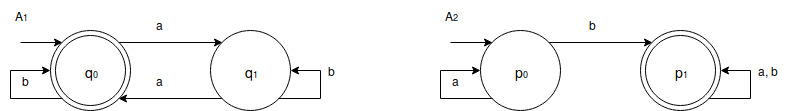
\includegraphics[width=1\textwidth]{a1a2}
\end{figure}
Ora costruiamo l'\emph{automa prodotto} rappresentando tutte le possibili combinazioni di stati che i due automi possono assumere in qualsiasi istante. Lo stato iniziale  \`e lo stato che ha come combinazione gli stati iniziali degli automi di partenza.\newline
Per capire come aggiungere gli archi consideriamo lo stato $(q_0, p_0)$, iniziamo chiedendoci in che stato l'automa deve transitare se l'input \`e $a$. \newline
$\delta_3((q_0, p_0),a)=(\delta_1(q_0,a),\delta_2(p_0,a))=(q_1,p_0)$, quindi aggiungiamo l'arco etichettato $a$ da $(q_0, p_0)$ a $(q_1,p_0)$. Con la stessa logica aggiungiamo tutti gli archi e otteniamo il seguente automa.\newline
Ora dobbiamo decidere quali sono gli stati finali. Dato che vogliamo ottenere l'unione dei due linguaggi gli stati finali sono quelli che nella propria etichetta contengono almeno uno stato finale degli automi di partenza.
\begin{figure}[H]
  \centering
    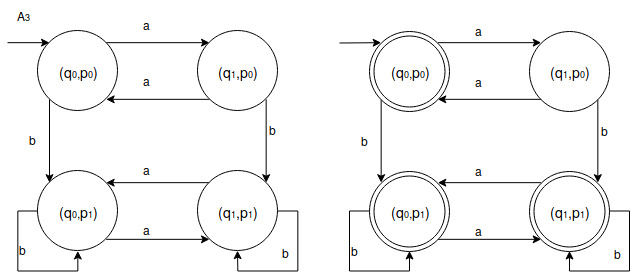
\includegraphics[width=1\textwidth]{a3}
\end{figure}

\newpage
%!TEX root=../../root.tex

\section{Lezione 3}
\subsection{Operazioni tra linguaggi regolari}
Siano $A_1$ e $A_2$ due automi a stati finiti possiamo definire un automa $A$ che accetti il risultato di una certa operazione tra il linguaggio di $A_1:$ e il linguaggio di $A_2$.
Per ogni operazione binaria possiamo definire l'automa come segue:
\[
	A = (Q_1 \times Q_2, \Sigma, \delta, q_0, F)
\]
\[
	\delta = (Q_1 \times Q_2) \times \Sigma \to Q_1 \times Q_2
\]
Definita come segue:
\[
	\delta ((q_1, q_2), a) = (\delta_1 (q_1, a), \delta_2 (q_2, a) )
\]
\[
	q_0 = (q_0^1, q_0^2)
\]
Possiamo definire anche $\delta^{\star}$:
\[
	\delta^{\star} ( (q_1, q_2), x) = (\delta_1^{\star} (q_1, x), \delta_2^{\star} (q_2, x))
\]
Ora definiamo F per le due operazioni binarie.
\subparagraph{Unione di linguaggi regolari}
\[
	\exists A \in DFA \; L(A)=L(A_1) \cup L(A_2)
\]
\[
	Q = \{ (q_1, q_2) | q_1 \in Q_1 \land q_2 \in Q_2 \}
\]
\[
	F = (Q_1 \times F_2) \cup (F_1 \times Q_2)
\]
\subparagraph{Intersezione di linguaggi regolari} 
\[
	\exists A \in DFA \; L(A)=L(A_1) \cap L(A_2)
\]
\[
	Q = \{ (q_1, q_2) | q_1 \in Q_1 \land q_2 \in Q_2 \}
\]
\[
	F = F_1 \times F_2 
\]
\subparagraph{Complemento di un linguaggio regolare} Definiamo separatamente il complemento di un linguaggio regolare.
\[
	L \in REG \Rightarrow \exists A \in DFA t.c. L(A) = L
\] 
\[
	A = (Q, \Sigma, \delta, q_0, F)
\] 
\[
	A^c = (Q, \Sigma, \delta, q_0, Q-F)
\]
\[
	L(A) \in REG \Leftrightarrow L^c(A) \in REG
\]

\subsection{Problemi di riduzioni, da automi a grafi}
Per rispondere ad alcune domande sugli automi \`e comodo ridurre il problema ad un problema sui grafi.\newline
\begin{description}
	\item \emph{Esempio 1}: dato un automa $A$ vogliamo sapere se $L(A)$ \`e finito, questo problema si pu\`o ridurre alla ricerca di un ciclo in un grafo. Per applicare l'algoritmo di ricerca dei cicli dobbiamo avere un \emph{automa ridotto}, ossia un grafo che rappresenti l'automa solamente con stati che appartengono a cammini da $q_0$ ad un qualsiasi stato in $F$ o da un qualsiasi stato in $F$ a $q_0$. 

	\item \emph{Esempio 2}: dato un automa $A$ vogliamo sapere se $L(A)=\emptyset$, questo problema si pu\`o ridurre alla ricerca di un percorso da $q_0$ ad un qualsiasi stato in $F$. Se non esistono cammini da $q_0$ ad un qualsiasi stato in $F$ allora $L(A)=\emptyset$.
\end{description}
Questi due problemi verranno discussi in dettaglio nella lezione 4.

\subsection{Operazioni su parole}
\subparagraph{Concatenazione} 
\begin{description}
	\item $x, y \in \Sigma^{\star} \Rightarrow xy \in \Sigma^{\star}$
	\item elemento neutro: $\varepsilon$, $x \varepsilon = x = \varepsilon x$
\end{description}
\subparagraph{Potenza}
\begin{description}
	\item $x \in \Sigma^{\star} \Rightarrow x^n = x. . .x $(x concatenata n volte con se stessa) $\in \Sigma^{\star}$
	\item elemento neutro: $1$, $x^1 = x$
	\item elemento cancellatore: $0$, $x^0 = \varepsilon$
\end{description}
\subsection{Operazioni su linguaggi}
\subparagraph{Concatenazione}
\begin{description}
	\item $L,L' \in REG \Rightarrow LL'=\{x | x \in \Sigma^{\star} \land \exists y \in L, z \in L' \land x=yz \}$
	\item elemento neutro: $\{\varepsilon\}$, $L \{\varepsilon\} = L =  \{\varepsilon\} L$
	\item elemento cancellatore: $\emptyset$, $L \emptyset = \emptyset =  \emptyset L$
\end{description}
\subparagraph{Potenza}
\begin{description}
	\item $L \in REG \Rightarrow L^n = \{ x^n | x \in L \land n \geq 0 \}$
	\item elemento neutro: $1$, $L^1 = L$
	\item elemento cancellatore: $0$, $L^0 = \{\varepsilon$\}
\end{description}
\subparagraph{Estensione o stella di Kleene}
\begin{description}
	\item $L^{\star} = \bigcup_{i \geq 0} L^i$
	\item Questa operazione fu introdotta nel 1976 da Robin e Scott.
\end{description}

\subsection{Automi non deterministici}
\subparagraph{In generale}
Un automa a stati finiti non deterministico, in breve NFA, \`e un automa in cui esistono passi di calcolo non \`e univocamente determinati.\newline
Immaginiamo di avere una macchina per il seguente automa:
\begin{figure}[H]
	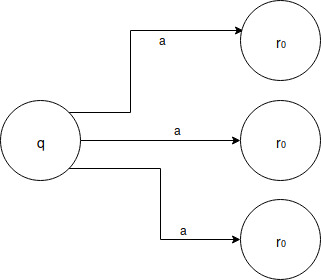
\includegraphics[scale=0.5]{nfa0}
\end{figure}
Possiamo immaginare la macchina eseguire i passi che corrispondono ad una sequenza di input e per ogni passo non univocamente determinato abbiamo delle macchine equivalenti che proseguono la computazione parallelamente per ogni possibile scelta di passo successivo.\newline
Introduciamo ora il concetto di \emph{configurazione}, sostanzialmente \`e un' estensione del concetto di stato e consiste nella coppia $(q, x)$ dove $q$ \`e uno stato dell'automa e $x$ \`e la parola in input allo stato $q$.\newline
Utilizzando le configurazioni possiamo rappresentare l'albero della computazione. Notare che nel caso di DFA abbiamo un albero degenere.
\subparagraph{Primi esempi}
\begin{description}
	\item \emph{Esempio 1}: $L =  \{x1y | x \in \Sigma^{\star} \land y \in \Sigma^2\}$, ossia tutte le stringhe che hanno $1$ come terzultimo simbolo.\newline
	Automa:
	\begin{figure}[H]
		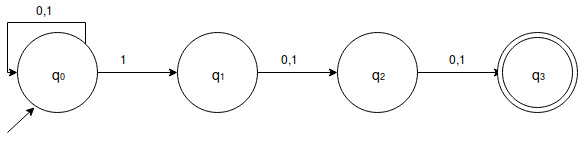
\includegraphics[scale=0.7]{nfa1}
	\end{figure}
	Albero della computazione:
	\begin{figure}[H]
		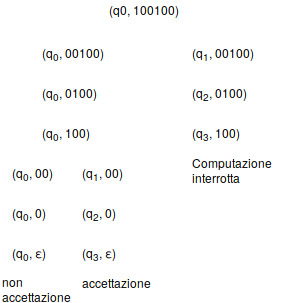
\includegraphics[scale=0.7]{nfa1alb}
	\end{figure}
	\item \emph{Esempio 2}: $L = \{ x0010 | x \in \Sigma^{\star}\} \cup \{ x100 | x \in \Sigma^{\star}\}$
	Automa:
	\begin{figure}[H]
		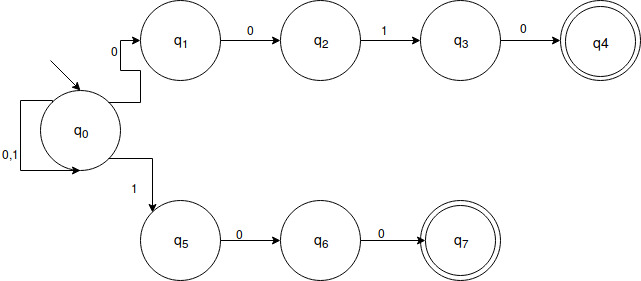
\includegraphics[scale=0.7]{nfa2}
	\end{figure}
\end{description}
\subsection{Dimostrazioni extra}
\subparagraph{Dimostrazione 1}

\[
	\delta^{\star} ( (q_1, q_2), x) = (\delta_1^{\star} (q_1, x), \delta_2^{\star} (q_2, x))
\]
Proviamo per induzione la precedente uguaglianza:\newline
Ricordiamo che la definizione di $\delta^{\star}$ \`e 
\begin{description}
	\item $\delta^{\star}(q, \varepsilon) = q \forall q \in Q$ 
	\item $\delta^{\star}(q, xa) = \delta(\delta^{\star}(q, x), a) \forall q \in Q, x \in \Sigma^{\star}, a \in \Sigma$
\end{description}
\begin{description}
	\item \emph{Passo base}: $x = \varepsilon$ \newline
	$\delta^{\star} ( (q_1, q_2), \varepsilon) = (q_1, q_2)$ per definizione di $\delta^{\star}$  ma $(q_1, q_2) = ( \delta(q_1, \varepsilon), \delta(q_2, \varepsilon))$
	\item \emph{Passo induttivo}: Supponiamo che l'uguaglianza valga per tutte le parole lunghe $n$, $(|x|=n, x \in \Sigma^{\star})$, e proviamo che valga per le parole lunghe $n+1$, $(xa, a \in \Sigma)$.
	\begin{description}
		\item $\delta^{\star} ((q_1, q_2), xa) = \delta ( \delta^{\star}((q_1, q_2),x), a)$ per definizione di $\Sigma^{\star}$
		\item $\delta ( ( \delta^{\star}((q_1, q_2),x), a) = \delta (( \delta_1^{\star}(q_1, x),\delta_2^{\star}(q_2,x)), a)$ per ipotesi induttiva
		\item $\delta ( (\delta_1^{\star}(q_1, x),\delta_2^{\star}(q_2,x)), a) = ( \delta_1 (\delta_1^{\star}(q_1, x),a), \delta_2(\delta_2^{\star}(q_2,x),a))$ per definizione di $\delta$
		\item $( \delta_1 (\delta_1^{\star}(q_1, x),a), \delta_2(\delta_2^{\star}(q_2,x),a)) = ( \delta_1^{\star}(q_1, xa), \delta_2^{\star}(q_2,xa))$ per definizione di $\delta^{\star}$ $\Box$
	\end{description}

\end{description}
\subparagraph{Dimostrazione 2}
Dati due automi $A_1 = (Q_1, \Sigma, \delta_1, q^1_0, F_1)$ con $L_1=L(A_1)$ e $A_2 = (Q_2, \Sigma, \delta_2, q^2_0, F_2)$ con $L_2=L(A_2)$ esiste $A = (Q = Q_1 \times Q_2, \Sigma, \delta, q_0, F = Q_1 \times F_2 \cup F_1 \times Q_2)$ tale che $L(A) = L(A_1) \cup L(A_2)$. Vogliamo dimostrare che:
\[
	x \in L(A) \Leftrightarrow x \in L(A_1) \lor x \in L(A_2)
\]
\[
	x \in L(A) \Leftrightarrow
\]
\[
	 \delta^{\star} ((q^1_0, q^2_0), x) \in F \Leftrightarrow
\]
\[	
	 (\delta_1^{\star}(q^1_0, x),\delta_1^{\star}(q^2_0, x)) \in F = Q_1 \times F_2 \cup F_1 \times Q_2) \Leftrightarrow 
\]
\[	 
	 \delta_1^{\star}(q^1_0, x) \in F_1 \lor \delta_1^{\star}(q^2_0, x) \in F_2 \Leftrightarrow 
\]
\[	 
	 x \in L(A_1) \lor x \in L(A_2) \Box
\]

\newpage
%!TEX root=../../root.tex

\section{Lezione 4}
\subsection{Algoritmi di problemi di riduzione}
\subparagraph{Algoritmo per linguaggio vuoto in DFA}
\begin{description}
	\item \emph{Input:} $A = (Q, \Sigma, \delta, q_0, F) \in DFA$
	\item \emph{Output:} s\`i se $L(A)=\emptyset$, no altrimenti
	\item \emph{Algoritmo:}\newline
		\begin{enumerate}
			\item Costruisci il grafo diretto $G=(V,E)$ cos\`i definito:
			\[
				V = Q \cup \{t | t \notin Q \}
			\]
			\[
				E = \{(p,q) | p, q \in Q \land \exists a \in \Sigma \land \delta(p, a) = q \} \cup \{(p,t) | p \in F\}			
			\]
			\item Verificare se c'\`e un cammino da $q_0$ a $t$; se s\`i rispondi no ($L(A)$ non vuoto), altrimenti rispondi s\`i
		\end{enumerate}
	\item \emph{Complessit\`a:} $\Theta (|Q|+|Q|\times|\Sigma|)$.
\end{description}
\subparagraph{Algoritmo per linguaggio finito in DFA}
\begin{description}
	\item \emph{Input:} $A = (Q, \Sigma, \delta, q_0, F) \in DFA$
	\item \emph{Output:} s\`i se $L(A)$ \`e finito, no altrimenti
	\item \emph{Algoritmo:}
		\begin{enumerate}
			\item Costruisci il grafo $G=(V,E)$ cos\`i definito:
			\[
				V = Q			
			\] 
			\[
				E = \{(p,q) | p, q \in Q \land \exists a \in \Sigma \delta(p,a) = q\}
			\]
			\item Elimina i nodi non raggiungibili da $q_0$ o dai quali non si raggiunge un nodo corrispondente ad uno stato finale.
			\item Verifica se G \`e aciclico; se s\`i rispondi s\`i ($L(A)$ \`e finito), altrimenti rispondi no.
	\item \emph{Complessit\`a:} $\Theta (|Q|+|Q|\times|\Sigma|)$.
		\end{enumerate}
\end{description}
\subsection{Definizione formale di NFA }
Possiamo definire un automa non deterministico esattamente come abbiamo fatto per gli automi deterministici, quello che cambia \`e la definizione della funzione $\delta$. Quindi un NFA \`e una quintupla $(Q, \Sigma, \delta, q_0, F)$ tale che: 
\[
	\delta : Q \times \Sigma \to {\cal P} (Q)
\]
Ossia $\delta (q,a) ={\cal P} (Q)$, quindi preso uno stato di partenza in $Q$ e un carattere $a \in \Sigma$ la funzione stabilisce in quale insieme di stati pu\`o transitare l'automa dopo la lettura di $a$. \newline
Notare che i $DFA$ sono casi particolari di $NFA$, ossia $NFA$ con stati singoletto.
\subsection{Da NFA a DFA}
Dopo aver capito l'utilit\`a di costruire automi non deterministici ci chiediamo se esiste un modo formale per costruire un automa deterministico partendo da un automa non deterministico.
\subparagraph{Teorema}
$	\forall A = (Q, \Sigma, \delta, q_0, F) \in NFA$ $\exists A'= (Q', \Sigma, \delta', q'_0, F') \in DFA$ tale che:
\begin{description}
	\item $Q' =  {\cal P}(Q)$
	\item $\forall X \in {\cal P}(Q)$ $\delta'(X,a) = \bigcup_{p \in X} \delta(p, a)$
	\item $q_0 = \{q_0\}$
	\item $F' = \{ X | X \in {\cal P}(Q) \land X \cap F \neq 0\}$
\end{description}
Notare che $|Q'| = 2^{|Q|}-1$.
\subparagraph{Algoritmo}
\begin{description}
	\item \emph{Input:} $A = (Q, \Sigma, \delta, q_0, F) \in NFA$
	\item \emph{Output:} $A' = (Q', \Sigma, \delta', q'_0, F') \in DFA$
	\item \emph{Algoritmo:}
		\begin{enumerate}[label*=\arabic*.]
			\item Poni $Q' = \{\{q_0\}\}$
			\item Ripeti finch\`e in $Q'$ ci sono stati non marcati
				\begin{enumerate}[label*=\arabic*.]
					\item Prendi un elemento non marcato $X \in Q'$
					\item Marca X
					\item $\forall a \in \Sigma$
						\begin{enumerate}[label*=\arabic*.]
							\item $Y_a = \bigcup_{p \in X} \delta(p,a)$
							\item $\delta'(X,a) = Y_a$
							\item $Y_a \notin Q' \Rightarrow$ aggiungi $Y_a$, non marcato, in $Q'$  						
						\end{enumerate}
					\item $\delta'(X,a)=Y$
					\item $Y \notin Q' \Rightarrow$ aggiungi $Y$, non marcato, a $Q'$
		
				\end{enumerate}
			\item $\forall X \in {\cal P}(Q) - Q'$ $\delta'(X, a) = \emptyset$ $ \forall a \in \Sigma$. Questo serve per rendere $\delta$ completo.
			\item Poni $q_0 = \{ q_0\}$ e $F' = \{X \in {\cal P}(Q) | X \cap F \neq \emptyset\}$
		\end{enumerate}
\end{description}

\subparagraph{Esempio}
Automa $A$ tale che $L(A) = \{x1ab | x 	\in \Sigma^{\star}\land a, b \in \Sigma \}$.
\begin{description}
	\item \emph{$NFA$:}
		\begin{figure}[H]
			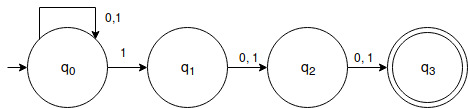
\includegraphics[scale=0.6]{nfadfa}
		\end{figure}
	\item \emph{$DFA$:}
		\begin{figure}[H]
			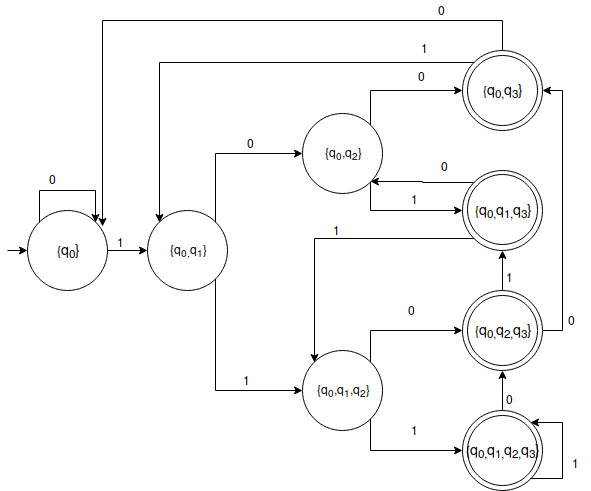
\includegraphics[scale=0.6]{nfadfa2}
		\end{figure}
\end{description}
\subsection{NFA con $\varepsilon$ mosse}
Vorremmo essere in grado di poter rappresentare dei cambi di stato non determinati da alcun input. Per far ci\`o usiamo la parola vuota. Pi\`u formalmente: 
\[
	A = (Q, \Sigma_{\varepsilon}, \delta, q_0, F)
\]
Dove:
\[
	\Sigma_{\varepsilon} = \Sigma \cup \{\varepsilon\}
\]
\[
	\delta : Q \times \Sigma_{\varepsilon} \to {\cal P}(Q)
\]
\begin{description}
	\item \emph{Esempio 1:} Ricerca stringhe nel testo. Sia $\Sigma = \{$ alfabeto inglese $\}$ vogliamo definire un $NFA$ $A$ tale che $L(A) = \{$ color, colour, web $\}$.
	\begin{figure}[H]
		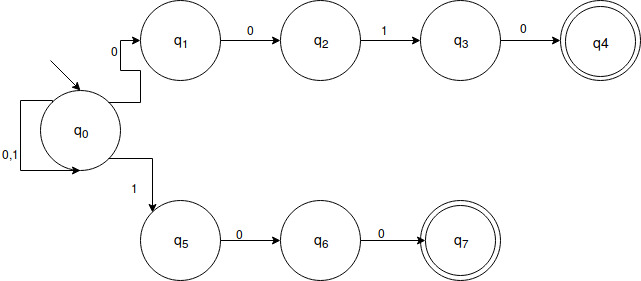
\includegraphics[scale=0.6]{nfa2}
	\end{figure}
	\item \emph{Esercizio 1:} Automa che riconosce i numeri reali.
\end{description}


\newpage
%!TEX root=../../root.tex


\section{Lezione 5}
\subsection{$\varepsilon$-mossa}
Introduciamo una mossa che permette la transizione di stato senza lettura di input. Non sempre la presenza della $\varepsilon$-mossa implica non determinismo.\newline
Ad esempio volendo costruire un automa che arrivato allo stato finale torni allo stato iniziale possiamo usare tale mossa senza creare non determinismo.\newline
\textbf{Esempio:}
\begin{figure}[H]
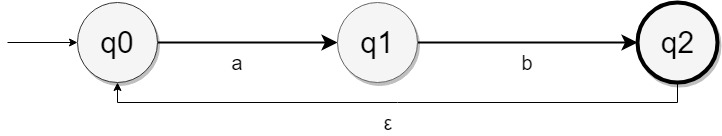
\includegraphics[scale=0.5]{l5_1}
\end{figure}
\subsection{Definizione formale di $NFA_{\varepsilon}$}
Ci\`o che cambia negli $NFA_{\varepsilon}$ \`e l'alfabeto di input, a $\Sigma$ viene aggiunta $\varepsilon$ che in questo caso rappresenta l'assenza di input. Quindi un $NFA_{\varepsilon}$ \`e una quintupla cos\`i definita:
\[
	A = (Q, \Sigma_{\varepsilon}, \lambda, q_0, F)
\]
Dove:
\[
	\Sigma_{\varepsilon} = \Sigma \cup \{\varepsilon\}
\]
\[
	\delta : Q \times \Sigma_{\varepsilon} \to {\cal P} (Q)
\]
Cambiando la definizione di $\delta$ dobbiamo ridefinire anche la funzione $delta^{\star}$:
\[
	\delta^{\star} (q, \varepsilon) = {q} \cup \delta(q, \varepsilon) 
\]
\[
	\delta^{\star} (q, xa) = \delta(\delta^{\star} (q, x), a)
\]
\textbf{Esempio:}
\begin{figure}[H]
	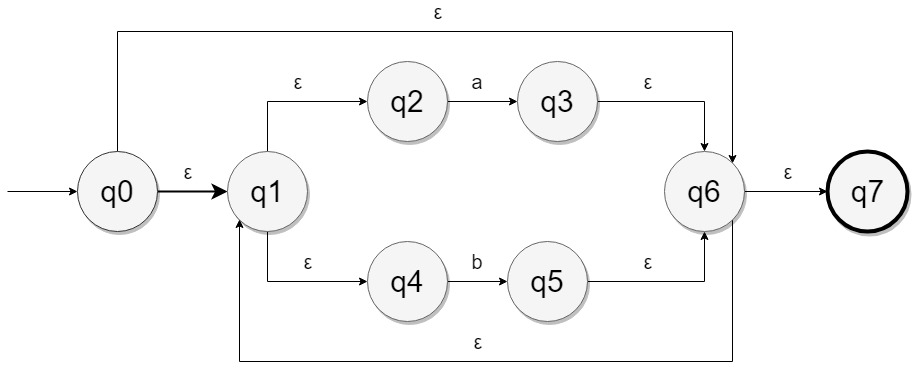
\includegraphics[scale=0.5]{l5_2}
\end{figure}

\subsection{Da $NFA_{\varepsilon}$ a $DFA$}
\subparagraph{Chiusura rispetto alla $\varepsilon$-mossa}

$\varepsilon - C(q)$ = insieme degli stati raggiungibili da q eseguendo solo $\varepsilon$ mosse.

Definiamo la chiusura di un insieme $X$ di stati rispetto alla $\varepsilon$-mossa come l'insieme degli stati raggiungibili con un numero arbitrario di $\varepsilon$ mosse da almeno uno stato nell'insieme $X$. Pi\`u formalmente:
\[
	\varepsilon-C(X) = \bigcup_{q \in X} \varepsilon-C(q)
\]

\subparagraph{Algoritmo}
\begin{description}
	\item \emph{Input:} $A = (Q, \Sigma_{\varepsilon}, \delta, q_0, F) \in NFA$
	\item \emph{Output:} $A' = (Q', \Sigma, \delta', q'_0, F') \in DFA$ tale che $L(A) = L(A')$
	\item \emph{Algoritmo:}
		\begin{enumerate}[label*=\arabic*.]
			\item Poni $Q' = \varepsilon-C(q_0)$
			\item Ripeti finch\`e in $Q'$ ci sono stati non marcati
				\begin{enumerate}[label*=\arabic*.]
					\item Prendi un elemento non marcato $X \in Q'$
					\item $\forall a \in \Sigma$
						\begin{enumerate}[label*=\arabic*.]
							\item $Y_a = \bigcup_{p \in X} \delta(p,a) \cup \varepsilon - C(p)$
							\item $\delta'(X,a) = Y_a$
							\item $Y_a \notin Q' \Rightarrow$ aggiungi $Y_a$, non marcato, in $Q'$  						
						\end{enumerate}
			\item $\forall X \in {\cal P}(Q) - Q' \Rightarrow \delta'(X, a) = \emptyset$ $ \forall a \in \Sigma$. Questo serve per rendere $\delta$ completo.
			\item Poni $q'_0 = \varepsilon - C(q_0)$ e $F' = \{Y \in Q' | Y \cap F \neq \emptyset\}$
				\end{enumerate}
		\end{enumerate}
\end{description}
\textbf{Esempio:} Il DFA che segue \`e il risultato dell'applicazione dell'algoritmo sull'NFA dell'esempio precedente. \newline
\begin{figure}[H]
	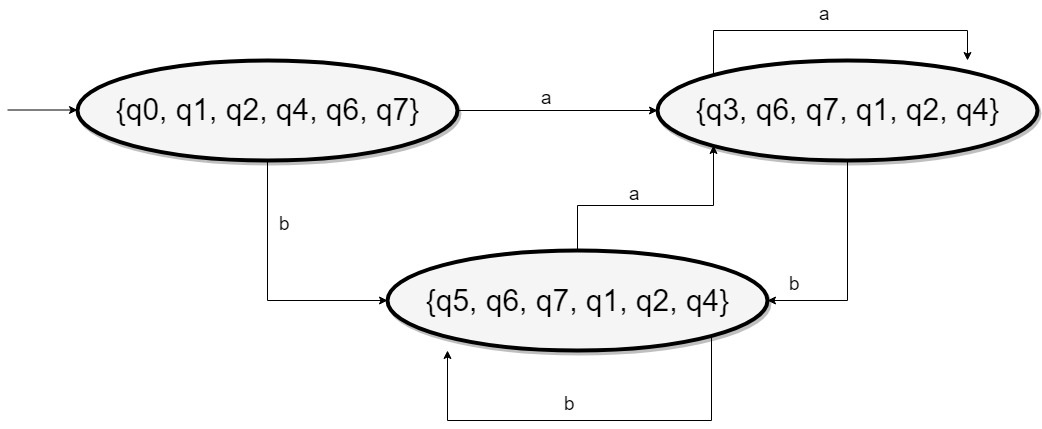
\includegraphics[scale=0.35]{l5_3}
\end{figure}
\subsection{Automa prodotto}
Siano $A_1$ e $A_2$ due automi cos\`i definiti:\newline
$A_1 = (Q_1, \Sigma, \delta_1, q^1_0,F_1)$ tale che $L = L(A_1)$ \newline $A_2 = (Q_2, \Sigma, \delta_2, q^2_0,F_2)$ tale che $L' = L(A_2)$  \newline
e che valga $Q_1 \cap Q_2 = \emptyset$. \newline
L'automa prodotto \`e $A = (Q_1 \cup Q_2, \Sigma_{\varepsilon}, \delta, q^1_0, F_2)$ con $\delta$ definita come segue:
\[
	A = (Q_1 \cup Q_2, \Sigma_{\varepsilon}, \delta, q_0^1, F_2)
\]
Dove:
\[
	\delta(q,a) = \delta_1(q,a) \forall  q \in Q_1-F_1, \forall a \in \Sigma_{\varepsilon}
\]
\[
	\delta(q,a) = \delta_1(q,a) \forall  q \in F_1, \forall a \in \Sigma
\]
\[
	\delta(q,\varepsilon) = \delta_1(q,\varepsilon) \cup {q_0^2} \forall  q \in F_1
\]
\[
	\delta(q,a) = \delta_2(q,a) \forall  q \in Q_2, \forall a \in \Sigma
\]

%\begin{figure}
	%\includegraphics[scale=0.5]{}
%\end{figure}

\subsection{Automa chiusura a stella di Kleene}
Siano $A'$ un automa cos\`i definito:\newline
$A' = (Q, \Sigma, \delta', q_0,F)$ tale che $L = L(A')$ \newline
L'automa che accetta $L^{\star}$ \`e definito come segue:
\[
	A = (Q \cup \{p_0\}, \Sigma_{\varepsilon}, \delta, q_0, F \cup \{p_0\})
\]
Dove:
\[
	p_0 \notin Q
\]
\[
	\delta(q,a) = \delta'(q,a) \forall  q \in Q-F, \forall a \in \Sigma
\]
\[
	\delta(p_0,\varepsilon) =  \{q_0\}
\]
\[
	\delta(q,a) = \delta'(q,a) \forall  q \in F_1, \forall a \in \Sigma
\]
\[
	\delta(q,\varepsilon) = \delta'(q,\varepsilon) \cup {q_0} \forall  q \in F_1
\]
\begin{figure}[H]
	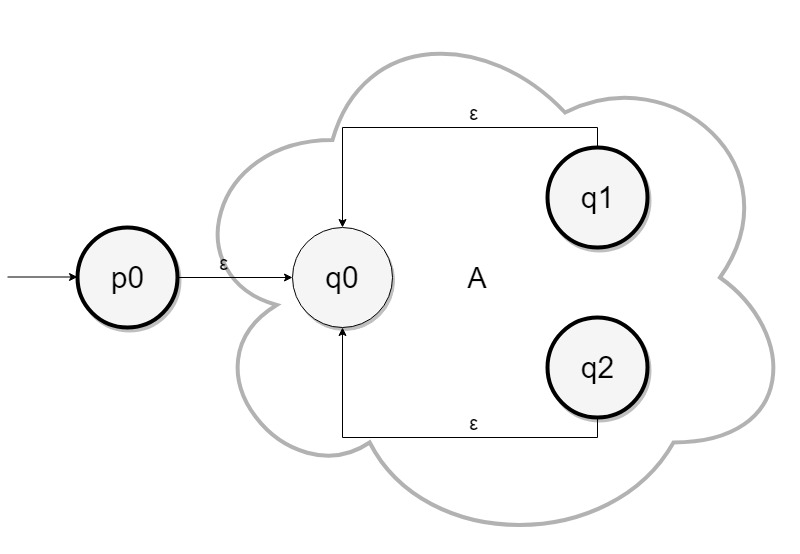
\includegraphics[scale=0.35]{l5_5}
\end{figure}
\textbf{Esempio:} Automa che riconosce il linguaggio $L = \{L^{\star}\}$
\begin{figure}[H]
	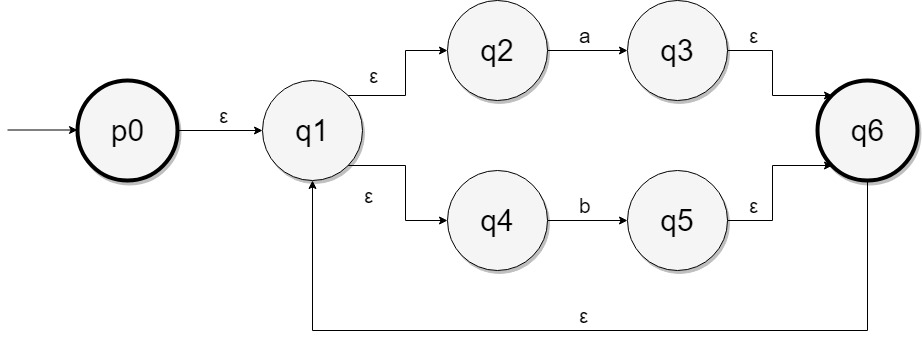
\includegraphics[scale=0.4]{l5_6}
\end{figure}

\subsection{Automa complemento}
Per ottenere l'automa complemento di un $NFA$ bisogna prima passare al $DFA$ equivalente e poi effettuare il complemento su di esso.


\newpage
%!TEX root=../../root.tex

\section{Lezione 6}
\subsection{Pumping lemma}
$L \in REG \Rightarrow \exists n > 0$ t.c. $\forall w \in L$  $|w| \geq n$ $\exists x, y, z$  $w = xyz$\newline
Vale:
\begin{enumerate}
	\item $|xy| \leq n$
	\item $|y| \geq 1$
	\item $\forall i \geq 0 xy^iz \in L$
\end{enumerate}
\textbf{Dimostrazione:}
$L \in REG \Rightarrow \exists A \in DFA$ che riconosce $L$ con $n$ stati. Sia $p \in L$ t.c. $|p| \geq n$, il cammino che determina in A \`e composto da almeno $n+1$ stati. Se il cammino \`e composto da un numero di nodi maggiore del numero degli stati vuol dire che in esso \`e presente un ciclo. Inoltre possiamo dire che questo ciclo si presenta necessariamente entro l'n-esimo passo di computazione poich\'e nella sequenza di nodi attraversati ci sar\`a necessariamente almeno una ripetizione.\newline
Questo lemma negato \`e utile per dimostrare la non regolarit\`a di un linguaggio.

\subsection{Pumping lemma negato}
$L \notin REG \Rightarrow \forall n > 0 \exists w \in L$ $|w| \geq n$ $\forall x, y, z$ t.c. $w=xyz$  \newline
Vale:
\begin{enumerate}
	\item $|xy| \leq n$
	\item $|y| \geq 1$
	\item $\exists i \geq 0 xy^iz \notin L$
\end{enumerate}

\subsection{Applicazione Pumping lemma negato}
\subparagraph{Esempio 1:} Dimostrare che $L= \{ ww | w \in \{0,1\}^{\star}\} \notin REG$. \newline
Dato $p \in \mathbb{N}$ vogliamo trovare una parola $w \in L$ t.c. $|w| \geq p$ e che per ogni sua scomposizione $w=xyz$ esiste un $i$ t.c. $W'=xy^iz \notin L$. \newline
Scriviamo in maniera generica $w$. Ad esempio $w = 0^p10^p1$, questa parola \`e evidentemente pi\`u lunga di $p$. \newline
Scegliamo come scomposizione $x = 0^r$,$y=0^s$,$z=0^{p-(r+s)}10^p$ con $r \geq 0$, $s \> 0$, $t \geq 0$.\newline
Adesso scriviamo $w'=xy^iz$ per la scomposizione che abbiamo scelto:
$0^r(0^s)^i0^{p-(r+s)}10^p1$.\newline
Affinch\'e $w' \notin L$ deve essere vero che: $r+is+p-(r+s) \neq p$, questo perch\`e vogliamo "rompere" la simmetria della parola. Semplificando otteniamo che $is-s \neq 0$ e questo \`e vero $\forall i \neq 1$.\newline
Pi\`u intuitivamente si pu\`o dire che per "rompere" la simmetrie basta elevare a 0 y per ottenere un numero di 0 nella prima met\`a della parola inferiore al numero di 0 nella seconda met\`a della parola.
\subparagraph{Esempio 2:} Dimostrare che $L = \{w | w \in \{a,b\}^{\star} \land n_a(w)=n_b(w)\} \notin REG$. \newline
Dato $p \in \mathbb{N}$ vogliamo trovare una parola $w \in L$ t.c. $|w| \geq p$ e che per ogni sua scomposizione $w=xyz$ esiste un $i$ t.c. $w'=xy^iz \notin L$.\newline
Procediamo scrivendo in maniera generica una parola che appartiene ad L. Ad esempio:\newline
$w=b^p a^p$, $|w| \geq p$ dato che $|b^p| = p$.\newline
Ora scomponiamo in maniera generica $w$:\newline
$x = b^r$, $y = b^s$, $z= b^t a^p$ t.c. $r \geq 0$, $s \> 0$, $t \geq 0$ e $r+s+t = p$.\newline
Adesso scriviamo $w'=xy^iz$ per la scomposizione che abbiamo scelto:
$b^r (b^s)^i b^t a^p$.\newline
Per ottenere $w' \notin L$ deve valere che $r+is+t \neq p$, ma questo \`e vero $\forall i \neq 1$. 
\subparagraph{Esempio 3:} Dimostrare che $L'=\{w | w \in \{a,b\}^{\star}\land n_a(w) \neq n_b(w)\} \notin REG$.\newline
Sta volta il Pumping lemma non ci aiuta e dobbiamo ragionare diversamente. Nell'esempio 3 \`e stato dimostrato che $L \notin REG$ ma $L=L'^c$ quindi possiamo concludere che $L' \notin REG$ poiché il suo complemento non \`e regolare. 
\subparagraph{Esempio 4:} Dimostrare che $L = \{ a^nb^m | n \neq m \land n,m \geq 0 \} \notin REG$.\newline
Per questo esempio di nuovo il Pumping lemma non ci aiuta. Proviamo a dimostrare la sua non regolarit\`a per assurdo. \newline
Supponiamo che $L \in REG$ e consideriamo un altro linguaggio che possiamo dimostrare non essere regolare sfruttando il Pumping lemma: $L' = \{a^nb^m | n=m \land n,m \geq 0 \}$. Definiamo ora il complemento di $L'$ come unione di $L$ e di un altro linguaggio. Essendo $L'$ il linguaggio delle parole formate da un certo numero di a seguite dallo stesso numero di b il suo complemento sar\`a formato da:
\begin{itemize}
	\item $L$, ossia tutte le parole che seguono l'ordinamento di $L'$ (a prima di b) in cui il numero di a differisce dal numero di b;
	\item $\{xbyaz | x, y, z \in \{a,b\}^{\star} \}$, ossia tutte le parole che non seguono l'ordinamento di $L'$. 
\end{itemize}
Ora possiamo scrivere che $L'^c = L \cup \{xbyaz | x, y, z \in \{a,b\}^{\star} \}$. Abbiamo supposto che $L \in REG$, sappiamo che $\{xbyaz | x, y, z \in \{a,b\}^{\star} \} \in REG$. La classe dei linguaggi regolari \`e chiusa rispetto all'unione quindi $L'^c \in REG$, ed \`e chiusa anche rispetto al complemento quindi $L' \in REG$. Questo \`e un assurdo in quanto sappiamo che $L' \notin REG$.
\newpage
%!TEX root=../../root.tex

\section{Lezione 7}
\subsection{Le espressioni regolari}
Le espressioni regolare, dall'inglese \emph{Regular Expression} in breve \textbf{RE}, sono un linguaggio formale alternativo agli automi. Le espressioni regolari denotano un linguaggio formale.
\subparagraph{Definizione induttiva}
\begin{description}
	\item \emph{Passo base:} 
		\begin{itemize}
			\item $\forall a \in \Sigma$ $a$ \`e una $RE$;
			\item $\varepsilon$ \`e una $RE$;
			\item $\emptyset$ \`e una $RE$.
		\end{itemize}
	\item \emph{Passo induttivo:} Se $R_1$ e $R_2$ sono $RE$ allora:
		\begin{itemize}
			\item $R_1 \cup R_2$ o $R_1 + R_2$ \`e una $RE$;
			\item $R_1R_2$ \`e una $RE$;
			\item $R_1^{\star}$ \`e una $RE$.
		\end{itemize}
\end{description}
\subparagraph{Linguaggi denotati da RE}
	\begin{description}
		\item $a \in \Sigma$ denota $L=\{a\}$;
		\item $\varepsilon$ denota $L=\{\varepsilon\}$;
		\item $\emptyset$ denota $L=\emptyset$;
		\item $L(R_1+R_2) = L(R_1) \cup L(R_2)$;
		\item $L(R_1R_2) = L(R_1)L(R_2)$;
		\item $L(R_1^{\star}) = (L(R_1))^{\star}$.
	\end{description}
Ricordiamo che:
\begin{description}
	\item $R \emptyset = \emptyset = \emptyset R$;
	\item $\emptyset^0 = \{\varepsilon\}$;
	\item $\emptyset^{\star} = \{\varepsilon\}$, questo rappresenta l'unico caso in cui l'operazione della stella di Kleene restituisce un insieme finito.
\end{description}
\subsection{Da $RE$ a $NFA$}
Data $R \in RE \Rightarrow \exists A \in NFA$ t.c. $L(R) = L(A)$.
\subparagraph{Dimostrazione:} per dimostrare questa implicazione ci baseremo sulla definizione induttiva di $RE$.
\begin{description}
 	\item Passo base:
 		\begin{itemize}
 			\item $a \in \Sigma \Rightarrow$ possiamo rappresentare $a$ come un automa costituito da un arco etichettato $a$ tra lo stato inziale $q_i$ e lo stato finale $q_f$.
 			\item $\varepsilon \in \Sigma \Rightarrow$ possiamo rappresentare $\varepsilon$ come un automa costituito dallo stato iniziale che \`e anche finale.
 			\item  $\emptyset \Rightarrow$ possiamo rappresentarlo come un automa costituito dal solo stato iniziale.
 		\end{itemize}
 	\item Passo induttivo:
 		\begin{itemize}
 			\item $R_1 \cup R_2 \Rightarrow \exists A_1 , A_2 \in NFA$ t.c. $L(A_1) = L(R_1) \land L(A_2) = L(R_2) \land L(A_1 \cup A_2 ) = L(R_1 \cup R_2 )$.
 			\item $R_1 + R_2 \Rightarrow$ come sopra ma con l'intersezione.
 			\item  $R_1^{\star} \Rightarrow \exists A_1$ t.c. $L(A_1) = L(R_1) \Rightarrow L(A_1)^{\star} = L(R_1)^{\star} \Rightarrow L(A_1^{\star}) = L(R_1^{\star})$.
 		\end{itemize}
\end{description}

\subsection{Da $DFA$ a $RE$}
Dato $A \in DFA \Rightarrow \exists R \in RE$ t.c. $L(A) = L(R)$.
\subparagraph{Dimostrazione:} per dimostrare questa implicazione esibiremo un algoritmo che dato un $DFA$ fornisce la $RE$ equivalente e motiveremo la sua correttezza.
\begin{description}
	\item \emph{Input:} $A = (Q, \Sigma, \delta, q_0 , F ) \in DFA$
	\item \emph{Output:} $R \in RE$ t.c. $L(R) = L(A)$
	\item \emph{Algoritmo:}
		\begin{enumerate}
			\item Trasformare $A$ in un $GNFA$ in forma normale.
			\item Ripeti l' eliminazione di uno stato finch\'e resta solo la coppia di stati iniziale e finale, $(q_0 , q_f )$.
			\item L'etichetta che resta sulla transizione dallo stato iniziale a quello finale \`e la $RE$ che denota il linguaggio accettato da $A$.
		\end{enumerate}
\end{description}
\textbf{\emph{GNFA in forma normale:}}\newline
$GNFA$ sta per \emph{Generalized NFA}, ossia un automa in cui ogni transizione \`e etichettata con una RE. Un $GNFA$ per essere in forma normale deve avere le seguenti
propriet\`a:
\begin{enumerate}
	\item Esiste un unico stato finale diverso da quello iniziale.
	\item Lo stato iniziale non deve avere archi entranti.
	\item Lo stato finale non deve avere archi uscenti.
	\item Tra ogni coppia di stati esiste un unico arco.
	\item Tra ogni coppia di stati esiste almeno un arco. Quest'ultima propriet\`a serve per rendere $\delta$ completa, quindi per ogni coppia di stati non legata da nessun arco bisogna aggiungere un arco etichettato $\emptyset$.
\end{enumerate}
\textbf{\emph{Passo di eliminazione di uno stato:}}\newline
Dato uno stato $q \in Q$ vogliamo eliminarlo senza cambiare il linguaggio accettando dall'automa. Per ogni $u, s \in Q $ t.c. esiste un cammino da $u$ ad $s$ passante per $q$ e di lunghezza 3, creo un arco da $u$ ad $s$ etichettato dalla $RE$ che consentiva di transitare da $u$ ad $s$ passando per $q$.\newline
\textbf{\emph{Correttezza:}}\newline
La correttezza di questo algoritmo risiede nel fatto che ad ogni passo di eliminazione il linguaggio accettato dall'automa non viene alterato. Per tale motivo al termine delle eliminazioni avremo una sola etichetta tra lo stato iniziale e quello finale, tale etichetta \`e proprio la $RE$ che denota il linguaggio accettato dall'automa.

\newpage
%!TEX root=../../root.tex

\section{Lezione 8}
\subsection{Context Free Grammar}
\subparagraph{Introduzione} Una $GFG$, \emph{[Contex Free Grammar]} , \`e un meccanismo che consente di generare tutte le parole di un certo linguaggio. Quindi date delle regole di derivazione, delle variabili e dei terminali dobbiamo essere in grado di applicare le regole ripetutamente partendo da una variabile di partenza fino ad arrivare ad una stringa composta da terminali che corrisponde ad una parola del linguaggio descritto dalla $CFG$.\newline
Le $GCF$ sono applicate nello sviluppo di parser per i compilatori poich\`e consentono di effettuare un analisi sintattica dei programmi.
\subparagraph{Definizione formale} Una grammatica $G$ \`e una quadrupla cos\`i definita:
\[
	G = (V, \Sigma, R, S)
\]
Dove:
\begin{description}
	\item $V$ \`e un insieme finito di \emph{variabili};
	\item $\Sigma$ \`e un insieme finito di \emph{terminali};
	\item $R$ \`e un insieme finito di \emph{regole};
	\item $S \in V$ \`e la \emph{variabile di partenza}.
\end{description}
Definiamo anche una relazione binaria $\Rightarrow \subseteq (V \times (V \cup \Sigma)^{\star})$. Questa relazione \`e ci\`o che ci consente di effettuare una sostituzione mediante l'uso delle regole, ad esempio siano $u, v, w \in (V \cup \Sigma)^{\star}$ e $S \in V$ allora $uSv \Rightarrow uwv$. \newline
Sfruttando questa relazioni possiamo anche definire il concetto di \emph{derivazione}, che consiste in una sequenza di sostituzioni, e indicheremo con $\Rightarrow^{\star}$.\newline
Una derivazione pu\`o essere descritta anche dall'\emph{albero di derivazione}. La radice \`e sempre la variabile di partenza, i figli della radice sono il risultato della prima sostituzione. Ogni nodo se \`e un terminale allora non pu\`o pi\`u essere derivato e quindi \`e una foglia, se \`e una variabile viene effettuata una sostituzione e i suoi figli sono il risultati e a seconda delle regole possono essere altre variabili e/o terminali.

\subparagraph{Esempi}
\begin{description}
	\item \emph{Esempio 1:} Grammatica per il linguaggio delle parole palindrome $PAL = \{x|x \in {0,1}^{\star} \land x=x^{rev}\}$.
		\begin{description}
			\item Variabili: $V = \{S\}$
			\item Terminali: $\Sigma = \{0, 1\}$
			\item Regole: $R = \{ S \to 0 | 1 | \varepsilon$, $S \to 0S0 | 1S1 \}$
			\item Variabile di partenza: $S$
		\end{description}
	\item \emph{Esempio 2:} Grammatica per il linguaggio $L=\{0^n1^n n \geq 0\}$.
		\begin{description}
			\item Variabili: $V = \{S\}$
			\item Terminali: $\Sigma = \{0, 1\}$
			\item Regole: $R = \{ S \to \varepsilon$, $S \to 0S1 \}$
			\item Variabile di partenza: $S$
		\end{description}
	\item \emph{Esempio 3:} Grammatica per il linguaggio per le operazioni aritmetiche.
		\begin{description}
			\item Variabili: $V = \{E, I\}$
			\item Terminali: $\Sigma = \{a, b, (, ), +, \times\}$
			\item Regole: $R = \{ E \to I | (E) | E+E | E \times E$, $I \to a | b \}$
			\item Variabile di partenza: $E$
		\end{description}
\end{description}

\newpage
%!TEX root=../../root.tex

\section{Lezione 9}
\subsection{La classe dei linguaggi descrivibili dalle CFG}
Possiamo ora definire una nuova classe di linguaggi, ossia quelli denotati dalle grammatiche context free. 
\[
	L(CFG) = \{ L | \exists G \in CFG \land L(G) = L \}
\]
Come la classe dei linguaggi regolari, anche questa classe gode di alcune propriet\`a di chiusura rispetto a delle operazioni che ci consentono di creare grammatiche complesse sulla base di grammatiche semplici.
\begin{description}
	\item \emph{Unione:} Dati $L, L' \in L(CFG) \Rightarrow L \cup L' \in L(CFG)$ \newline Siano $G_1 = (V_1, \Sigma, R_1, S_1) \in CFG$ e $G_2= (V_2, \Sigma, R_2, S_2)$ definiamo l'unione delle due grammatiche come segue: $G_1 \cup G_2 = (V_1 \cup V_2, \Sigma, R_1 \cup R_2 \cup \{ S \to S_1 | S_2\}, S)$. Aggiungendo la regola $S \to S_1 | S_2$ stiamo imponendo che la prima derivazione sia la o la variabile di partenza di $G_1$ o quella di $G_2$. Notare che non vogliamo che le regole si mescolino per tale motivo deve valere che $V_1 \cap V_2 = \emptyset$.
	\item \emph{Prodotto:} Dati $L, L' \in L(CFG) \Rightarrow LL' \in L(CFG)$\newline Siano $G_1 = (V_1, \Sigma, R_1, S_1) \in CFG$ e $G_2= (V_2, \Sigma, R_2, S_2)$ definiamo il prodotto delle due grammatiche come segue: $G_1 G_2 = (V_1 \cup V_2, \Sigma, R_1 \cup R_2 \cup \{ S \to S_1S_2\}, S)$. Aggiungendo la regola $S \to S_1S_2$ stiamo imponendo che la prima derivazione sia la concatenazione delle variabili di partenza di $G_1$ e di $G_2$. Per lo stesso motivo di prima $V_1 \cap V_2 = \emptyset$. 
\end{description}
\subparagraph{Esempio:}  Dato il linguaggio $L = \{ 0^n1^m | n \neq m \land n, m \geq 0\}$ vogliamo trovare una grammatica per $L$ scomponendolo in linguaggi pi\`u semplici, per i quali trovare una grammatica sia facile, per poi unirle ed ottenere una grammatica per $L$. \newline Possiamo scrivere $L$ come l'unione dei seguenti linguaggi: 
\begin{description}
	\item $L_1 = \{0^n, n \geq 1\}$, per il quale possiamo definire la grammatica con le seguenti regole $R_1 = \{S_0 \to 0|0S_0\}$ con $S_0$ variabile di partenza.
	\item $L_2 = \{1^m, m \geq 1\}$, per il quale possiamo definire la grammatica con le seguenti regole $R_2 = \{S_1 \to 1|1S_1\}$ con $S_1$ variabile di partenza.
	\item $L_3 = \{0^n1^m,  n > m > 0\}$ che senza perdita di generalit\`a possiamo riscrivere come $L_3 = \{0^{m+p}1^m, m, p > 0\}$, per il quale possiamo definire la grammatica con le seguenti regole $R_3 = \{S_2 \to S_0S', S' \to 0S'1 | 01\}$ con $S_2$ variabile di partenza.
	\item $L_4 = \{0^n1^m  m > n > 0\}$ che senza perdita di generalit\`a possiamo riscrivere come $L_3 = \{0^n1^{n+p}, n, p > 0\}$, per il quale possiamo definire la grammatica con le seguenti regole $R_4 = \{S_3 \to S'S_1\}$ con $S_3$ variabile di partenza.
\end{description}
Notare che, sapendo di dover fare l'unione, alcune variabili delle grammatiche che descrivono i linguaggi semplici $L_i, i \in \{1,2,3,4\}$ sono definite in un solo linguaggio e poi riutilizzate negli altri, ad esempio $S_0$ o $S'$. \newline
Combinando le regole scritte per il linguaggi semplici otteniamo che la grammatica per $L$ \`e $G = (V, \Sigma, R, S)$ dove: 
\begin{description}
	\item $V = \{S, S_0, S_1, S_2, S_3, S'\}$;
	\item $\Sigma = \{0, 1\}$;
	\item $R = \{ S \to S_0 | S_1 | S_2 | S_3$, $S_0 \to 0|0S_0$, $S_1 \to 1|1S_1$, $S_2 \to S_0S'$, $S_3 \to S'S_1$, $S' \to 0S'1 | 01\}$.
\end{description}
\subsection{Grammatiche ambigue}
Intanto diciamo che una \emph{derivazione leftmost} o \emph{derivazione canonica a sinistra} \`e una derivazione in cui l'ordine di derivazione da precedenza alle variabili scritte pi\`u a sinistra.\newline
Una grammatica $G$ si dice \emph{ambigua} se esiste almeno una parola in $L(G)$ che pu\`o essere derivata con almeno due diverse derivazioni leftmost.\newline
Data una grammatica ambigua $G$, ottenere $G'$ non ambigua ed equivalente a $G$ non \`e algoritmicamente risolvibile.\newline
Esistono anche \emph{linguaggi intrinsecamente ambigui}, ossia non esiste grammatica non ambigua che li genera. Ad esempio $L = \{a^ib^jc^k | i=j o j=k, i, j, k \geq 0 \}$
\subparagraph{Gestire l'ambiguit\`a} Segue un esempio di come modificare una grammatica ambigua per il linguaggio delle espressioni aritmetiche per renderla non ambigua.\newline
Data la grammatica $G = (V, \Sigma, R, E)$ dove:
\begin{description}
	\item $V = \{E, I\}$;
	\item $\Sigma = \{a, b, (, ), +, \times \}$;
	\item $R = \{ E \to (E) | E + E | E \times E | I, I \to a | b\}$;	
\end{description}
Possiamo vedere che \`e possibile ricavare l'espressione $a + b \times b$ attraverso due diverse derivazioni leftmost:\newline
\begin{description}
	\item $E \Rightarrow E \times E \Rightarrow E + E \times E \Rightarrow a + E \times E \Rightarrow a + b \times E \Rightarrow a + b \times b $
	\item $E \Rightarrow E + E \Rightarrow a + E \Rightarrow a + E \times E \Rightarrow a + b \times E \Rightarrow a + b \times b $ 
\end{description}
Modifichiamo ora la grammatica in modo che non risulti pi\`u ambigua:
\begin{description}
	\item $V = \{E, T, F, I\}$, dove T la possiamo interpretare come la variabile dei termini e F la come la variabile dei fattori;
	\item $\Sigma = \{a, b, (, ), +, \times \}$;
	\item $R = \{ E \to T | E + T, T \to F | T \times F, F \to I | (E), I \to a | b\}$;	
\end{description}
\subsection{Problemi decidibili e indecidibili}
Un problema si dice \emph{decidibile} se esiste un algoritmo che lo risolve.\newline
Un problema si dice \emph{indecidibile} se non esiste un algoritmo che lo risolve. \newline
Seguono esempi di problemi:
\begin{description}
	\item \emph{Problema 1:} Disambiguazione di una grammatica \`e un problema indecidibile
	\item \emph{Problema 2:} Dati $A_1, A_2 \in DFA$ dire se $L(A_1) \subseteq L(A_2)$ \`e decidibile. S\`i, possiamo riformulare $L(A_1) \subseteq L(A_2)$ come $L(A_1) \cup L(A_2)^c = \emptyset$ che sappiamo essere un problema decidibile
	\item \emph{Problema 3:} Dati $A_1, A_2 \in DFA$ dire se $L(A_1) = L(A_2)$ \`e decidibile? S\`i, perch\`e $L(A_1) = L(A_2) \Leftrightarrow L(A_1) \subseteq L(A_2) \land L(A_2) \subseteq L(A_1)$. 
	\item \emph{Problema 4:} Dato $A \in DFA$ dire se $L(A) = \Sigma^{\star}$ \`e decidibile. S\`i e possiamo vedere il problema in due diversi modi. Il primo \`e ricondurlo all'equivalenza di due linguaggi. Il secondo \`e riformulare il problema come segue: $L(A)^c = \emptyset$.
	\item \emph{Problema 5:} Dati $A_1, A_2 \in DFA$ dire se esiste una parola $x$ t.c. $x \notin L(A_1) \land x \notin L(A_2)$. Anche questo problema \`e decidibile e pu\`o essere risolto in due diversi modi. Possiamo dire che $(L(A_1) \cup L(A_2))^c \neq \emptyset \Rightarrow \exists x$ t.c. $x \notin L(A_1) \land x \notin L(A_2)$. Oppure possiamo risolvere verificando se almeno uno dei linguaggi \`e uguale a $\Sigma^{\star}$.
\end{description}

\newpage
%!TEX root=../../root.tex

\section{Lezione 10}
\subsection{Forma normale di Chomsky}
La forma normale di Chomsky \`e la pi\`u semplice e utile forma in cui esprimere una CFG.
Diciamo che una grammatica $G = (V, \Sigma, R, S)$ \`e nella forma normale di Chomsky se ogni regola in $R$ \`e nella forma: 
\[
	A \to BC | A, B, C \in V
\]
\[
	A \to a | A \in V, a \in \Sigma
\]
Inoltre Sipser aggiunge che sia permessa la regola cencellante:
\[
	S \to \varepsilon
\]
e che per limitare la lunghezza della derivazione $S$ non deve essere nella parte destra di nessuna regola.
\paragraph{Algoritmo per ottenere una grammatica in forma normale di Chomsky}
\begin{description}
	\item \emph{Input:} $G = (V, \Sigma, R, S) \in CFG$.
	\item \emph{Output:} $G' = (V', \Sigma, R', S')$ equivalente a $G$ ma in forma normale di Chomsky.
	\item \emph{Algoritmo:}
		\begin{enumerate}
			\setcounter{enumi}{-1}
			\item Dato che non vogliamo che la variabile di partenza $S$ compaia nella parte destra delle regole allora aggiungiamo $S_0$ in $V$ come variabile di partenza e la regola $S_0 \to S$.
			\item \textbf{Eliminazione delle regole cancellanti}
			\item \textbf{Eliminazione delle regole unitarie}
			\item \textbf{Eliminazione delle variabili e regole inutili}
			\item \textbf{Sostituzione delle regole con parte destra pi\`u lunga di tre e sostituzione dei terminali con delle variabili}
			\item Aggiungiamo la regola $S_0 \to \varepsilon$ se necessario.
		\end{enumerate}
		Notare che i passi 0 e 5 sono stati aggiunti da Sipser e la forma normale di Chomsky originale prevede solo i passi da 1 a 4.\newline
		Ora vediamo nel dettaglio i passi dal 1 al 4:
		\begin{enumerate}
			\item \textbf{Eliminazione delle regole cancellanti}
				\begin{description}
					\item \emph{Input:} $G = (V, \Sigma, R, S)$
					\item \emph{Output:} $G' = (V', \Sigma, R', S')$ equivalente a $G$ ma senza regole cancellanti
					\item \emph{Algoritmo:}
						\begin{itemize}
							\item Sia $NULL$ l'insieme delle variabili implicate in regole cancellanti.
							\item Definiamo inizialmente $NULL$ come $NULL_0 = \{ A | A \in V \land A \to \varepsilon \}$.
							\item Ripetiamo $NULL_i = NULL_{i-1} \cup \{ A | A \in V \land A \to u_1 ... u_k \in R \land u_j \in NULL_{i-1} 1 \leq j \leq k\}$ finch\'e $NULL_i \neq NULL_{i-1}$  o $NULL_i \neq V$.
							\item $\forall A \in NULL$, $\forall B \to uAv \in R$ t.c. $B \in V, u,v \in (V \cup \Sigma)^{\star}$ aggiungo una nuova regola $B \to uv$. Notare che se $u$ e $v$ sono composte interamente da variabili che appartengono a NULL allora possiamo direttamente non aggiungere la regola.
							\item Eliminiamo tutte le regole nella forma $A \to \varepsilon, \forall A \in NULL$.
						\end{itemize}		
				\end{description}
			\item \textbf{Eliminazione delle regole unitarie}
				\begin{description}
					\item \emph{Input:} $G = (V, \Sigma, R, S)$
					\item \emph{Output:} $G' = (V', \Sigma, R', S')$ equivalente a $G$ ma senza regole unitarie
					\item \emph{Algoritmo:}
						\begin{itemize}
							\item Sia $UNIT$ l'insieme delle variabili implicate in regole unitarie.
							\item Definiamo inizialmente $UNIT$ come $UNIT_0 = \{ (A,A) | A \in V\}$. Ossia stiamo considerando le regole unitarie implicite della forma $A \to A$ che equivale a non applicare nessuna regola in un passo di derivazione.
							\item Ripetiamo $UNIT_i = UNIT_{i-1} \cup \{ (A, C) | (A, B) \in UNIT_{i-1} \land B \to C \in R \}$ finch\'e $UNIT_i \neq UNIT_{i-1}$  o $UNIT_i \neq V$.
							\item $\forall (A, B) \in UNIT$ se esiste la regola $B \to u, u \in (V \cup \Sigma)^{\star}$ aggiungo la regola $A \to u$ ed elimino le regole unitarie.
						\end{itemize}
				\end{description}
			\item \textbf{Eliminazione delle variabili e regole inutili}
				Le variabili sono inutili se:
				\begin{enumerate}
					\item partendo da essa non \`e possibile derivare una stringa di terminali per qualsiasi numero di passi. Queste variabili sono chiamate \emph{variabili non produttive}.
					\item dalla variabile iniziale non \`e possibile derivarla. Queste variabili sono chiamate \emph{variabili non derivabili}.	
				\end{enumerate}
				Suddividiamo questo passo in due algoritmi che si occupano rispettivamente dell'eliminazione delle variabili non produttive e delle variabili non derivabili.\newline
				\textbf{Eliminazione delle variabili non produttive}
				\begin{description}
					\item \emph{Input:} $G = (V, \Sigma, R, S)$
					\item \emph{Output:} $G' = (V', \Sigma, R', S')$ equivalente a $G$ ma senza regole non produttive
					\item \emph{Algoritmo:}
						\begin{itemize}
							\item Sia $PROD$ l'insieme delle variabili produttive
							\item Definiamo inizialmente $PROD$ come $PROD_0 = \{ A | A \in V \land A \to u \in R \land u \in \Sigma^{Star}\}$. 
							\item Ripetiamo $PROD_i = PROD_{i-1} \cup \{ A | A \in V \land A \to u \in R \land u \in PROD_{i-1} \}$ finch\'e $PROD_i \neq PROD_{i-1}$  o $PROD_i \neq V$.
							\item Eliminiamo tutte le regole in cui occorrono elementi che appartengono a $V-PROD$.
						\end{itemize}
				\end{description}
			\textbf{Eliminazione delle variabili non derivabili}
				\begin{description}
					\item \emph{Input:} $G = (V, \Sigma, R, S)$
					\item \emph{Output:} $G' = (V', \Sigma, R', S')$ equivalente a $G$ ma senza regole non derivabili
					\item \emph{Algoritmo:}
						\begin{itemize}
							\item Sia $DER$ l'insieme delle variabili derivabili
							\item Definiamo inizialmente $DER$ come $DER_0 = \{S \}$. 
							\item Ripetiamo $DER_i = DER_{i-1} \cup \{ A | \exists B \in DER_{i-1} \land B \to uAv \in R \}$ finch\'e $DER_i \neq DER_{i-1}$  o $DER_i \neq V$.
							\item Eliminiamo tutte le regole in cui occorrono elementi che appartengono a $V-DER$.
						\end{itemize}
				\end{description}		
			\item \textbf{Sostituzione delle regole con parte destra pi\`u lunga di tre e sostituzione dei terminali con delle variabili}
				\begin{itemize}
					\item Se sono presenti regole del tipo $A \to u_1 ... u_k$ con $k \geq 3$ la sostituisco con una serie di regole di questa forma: 
					\[
						A \to u_1B_1					
					\]
					\[
						B_1 \to u_2B_2					
					\]
					\[
						...					
					\]
					\[
						B_{k-2} \to u_{k-1}u_k					
					\]
					\item $\forall u \in \Sigma$ aggiungiamo una nuova regola definendo una nuova variabile $U \to u$ e sostituiamo $U$ ad $u$ in tutte le regole in cui $u$ occorre nella parte destra (di lunghezza 2).
				\end{itemize}
		\end{enumerate}
\end{description}
\subparagraph{Esempio} Diamo ora un esempio completo dell'applicazione dell'algoritmo.\newline
Sia $G = (V, \Sigma, R, S)$ la seguente grammatica:
\begin{description}
	\item $V = \{S, A, B\}$
	\item $\Sigma = \{a, b\}$
	\item Le seguenti regole appartengono ad $R$:
	\[S \to ASB | \varepsilon \]
	\[A \to aAS | a \]
	\[B \to bSb | A | bb\]
\end{description}
\begin{enumerate}
	\setcounter{enumi}{0}
	\item Aggiungiamo una nuova variabile di partenza $S_0$ e la regola $S_0 \to S$, quindi $G$ \`e ora cos\`i definita:
	\begin{description}
		\item $V = \{S_0, S, A, B\}$
		\item $\Sigma = \{a, b\}$
		\item Le seguenti regole appartengono ad $R$:
		\[S_0 \to S\]
		\[S \to ASB | \varepsilon \]
		\[A \to aAS | a \]
		\[B \to bSb | A | bb\]
		\item $S_0$ variabile di partenza.
	\end{description} 
	\item L'unica regola cancellante \`e $S \to \varepsilon$. Quindi $NULL = \{S\}$. Procediamo aggiungendo le regole in cui S viene cancellato e otteniamo le regole $S \to AB, A \to aA$ quindi $R$ sar\`a cos\`i definito:
		\[S_0 \to S\]
		\[S \to ASB | AB \]
		\[A \to aAS | aA | a \]
		\[B \to bSb | A | bb\]
	\item Eliminiamo ora le regole unitarie.
		\begin{description}
			\item $UNIT_0 = \{(S_0, S_0), (S, S), (A, A), (B, B)\}$
			\item $UNIT_1 = UNIT_0 \cup \{ (S_0, S), (B,A)\}$
			\item $UNIT_2 = UNIT_1 \cup \emptyset$
			\item ora dobbiamo sostituire $S_0 	\to S$ con $S_0 \to ASB | AB$ e $B 	\to A$ con $B \to aAS | aA | a  $ e otteniamo il nuovo insieme di regole cos\`i definito:
			\[S_0 \to ASB | AB\]
			\[S \to ASB | AB \]
			\[A \to aAS | aA | a \]
			\[B \to bSb | aAS | aA | a | bb\]
		\end{description}
	\item Cerchiamo ora le variabili produttive e quelle derivabili.
		\begin{description}
			\item $PROD_0 = \{A, B\}$ 
			\item $PROD_1 = PROD_0 \cup \{S, S_0\}$
			\item $PROD_1 = V$ quindi mi fermo poich\`e non ci sono variabili non produttive.
			\item $DER_0 = \{S_0\}$
			\item $DER_1 = DER_0 \cup \{S, A, B\}$
			\item $DER_1 = V$ quindi mi fermo poich\`e non ci sono variabili non derivabili.
		\end{description}
		In questo passo la grammatica \`e rimasta invariata.
	\item Adesso introduciamo le variabili per le regole di derivazione dei terminali e aggiungiamo tali regole e infine riduciamo tutte le regole a regole con parte destra di lunghezza al pi\`u 2:
		\begin{description}
			\item Introducendo le regole dei terminali otteniamo:
			\[S_0 \to ASB | AB\]
			\[S \to ASB | AB \]
			\[A \to DAS | DA | D \]
			\[B \to CSC | DAS | DA | D | CC\]
			\[C \to b\]
			\[D \to a\]
			\item $S_0 \to ASB$ diventa $S_0 \to AF$ e viene quindi introdotta la variabile $F$ e la regola $F \to SB$. Similmente procediamo per tutte le regole con parte destra con lunghezza maggiore di 2 e otteniamo $R$ cos\`i definito:
			\[S_0 \to AF | AB\]
			\[F \to SB \]
			\[S \to AG | AB \]
			\[G \to SB \]
			\[A \to DH | DA | D \]
			\[H \to AS \]
			\[B \to CI | DJ | DA | D | CC\]
			\[I \to SC \]
			\[J \to AS \]
			\[C \to b\]
			\[D \to a\]		
		\end{description}
	\item Infine aggiungiamo la regola $S_0 \to \varepsilon$ poich\`e la parola vuota poteva essere derivata della grammatica iniziale.
\end{enumerate}
Quindi la nuova grammatica \`e cos\`i definita:
\begin{description}
	\item $V = \{S_0, S, A, B, C, D, F, G, H, I, J\}$
	\item $Sigma = \{a, b\}$
	\item Le seguenti regole appartengono ad $R$
	\[S_0 \to AF | AB\]
	\[F \to SB \]
	\[S \to AG | AB \]
	\[G \to SB \]
	\[A \to DH | DA | D \]
	\[H \to AS \]
	\[B \to CI | DJ | DA | D | CC\]
	\[I \to SC \]
	\[J \to AS \]
	\[C \to b\]
	\[D \to a\]	
	\item $S_0$ variabile di partenza
\end{description}
\subparagraph{Problema di decisione} Stabilire se una grammatica genera un linguaggio vuoto.\newline
Una grammatica non \`e vuota se ha almeno una variabile produttiva. Possiamo quindi ridurre questo problema alla ricerca di variabili produttive, se non troviamo alcuna variabile produttiva allora la grammatica genera un linguaggio vuoto, altrimenti no.\newline
Proviamo a dare un'idea della complessit\`a asintotica di questo algoritmo risolutivo. Possiamo dire che la grandezza della grammatica \`e data dal numero di variabili e dal numero di regole, quindi cerchiamo di esprimere la complessit\`a attraverso queste due grandezze. Sia $m = |V|$ e $n = |R|$. Il calcolo di $PROD_i$ \`e lineare nel numero di regole, infatti calcolando $PROD_i$ al massimo tutte le regole causeranno l'aggiunta di una variabile produttiva. Per calcolare $PROD$ al massimo sono necessarie $m$ iterazioni poich\`e una volta raggiunto $PROD = V$ non possiamo pi\`u aggiungere nulla. Quindi concludiamo che questo algoritmo ha complessit\`a $O(m \times n)$.

\newpage
%!TEX root=../../root.tex

\section{Lezione 11}
\subsection{Problema appartenenza per CFG}
Dato $G = (V, \Sigma, R, S)$ e $w \in \Sigma^{\star}$ vogliamo sapere se $w \in L(G)$. Sia $n = |w|$, se $G$ è in forma normale di Chomsky $w$ è derivabile in $2n-1$ passi, poiché abbiamo bisogno di $n-1$ passi per arrivare da $S$ a $A_1 \dots A_n$ e altri $n$ passi per arrivare da $A_1 ... A_n$ a $a_1 ... a_n$. Quindi dato che le le derivazioni di parole lunghe $n$ sono lunghe $2n-1$ passi possiamo cercare $w$ tra tutte le derivazioni lunghe $2n-1$ passi. 
---manca complessità---
\subsection{Automi a pila}
Gli \textit{automi a pila} o $PDA$ (\textit{Push Down Automata}) sono un'estensione del concetto di $NFA$ che ci permettono di esprimere i linguaggi espressi dalle CFG. Ciò che hanno di nuovo è una pila che fornisce la possibilità di memorizzare più informazioni e quindi effettuare scelte più complesse. Ciò consente agli automi di riconoscere alcuni linguaggi non regolari. La pila viene acceduta in cima, sia in lettura che in scrittura, è inizialmente vuota e ogni volta che si "toglie" un carattere dalla pila, l'informazione è persa, così come ogni volta che si "mette" un carattere nella pila, prima di potervi accedere bisogna leggere e togliere i caratteri impilati successivamente.
\paragraph{Definizione formale}
Un $PDA$ è una sestupla
\[A = (Q, \Sigma, \Gamma, \delta, q_0, F)\]
Dove:
\begin{itemize}
	\item $Q$ è l'insieme degli stati
	\item $\Sigma$ è l'alfabeto di input
	\item $\Gamma$ è l'alfabeto sulla pila (che può coincidere con l'alfabeto di input);
	\item $\delta$ è la funzione di transizione: 
	$$\delta : Q \times \Sigma_{\varepsilon} \times \Gamma_{\varepsilon} \to \mathcal{P} ( Q \times \Gamma_{\varepsilon} )$$ Ossia dato uno stato di partenza $q \in Q$, un carattere letto in input $a \in \Sigma_{\varepsilon}$ e il carattere da leggere in cima alla pila $b \in \Gamma_{\varepsilon}$ la funzione $\delta$ ci dice l'insieme di stati in cui transitare e il relativo carattere da scrivere al posto del carattere letto. Quindi $\delta(q,a,x) = {(p,y), (r,z)}$ significa che da $q$ dopo aver letto $a$ possiamo transitare o in $p$ sostituendo $y$ ad $x$ in cima alla pila oppure in $r$ sostituendo $z$ ad $x$ in cima alla pila. Se $a = \varepsilon$ siamo aggiungendo un elemento in cima alla pila. Se $y = \varepsilon$ allora stiamo eliminando $a$ dalla cima della pila
	\item $q_0$ è lo stato iniziale
	\item $F$ è l'insieme degli stati finali
\end{itemize}

\paragraph{Classe dei linguaggi riconosciuti dai $PDA$}
Definiamo la classe e dei linguaggi riconosciuti dai $PDA$ come:
$$L(PDA) = \{L | \exists A \in PDA \land L(A) = L\}$$
\paragraph{Configurazioni in PDA}
Come negli automi a stati finiti anche nei PDA esiste il concetto di configurazione, in questo caso è una tripla $(q, x, w)$ dove:
\begin{itemize}
 \item  $q$ è lo stato corrente
 \item $x$ è la parola in input da leggere
 \item e $w$ è il contenuto della pila (il carattere più a sinistra è quello in cima alla pila)
 \end{itemize}
 Definiamo la relazione binaria "\textit{porta a}" $\Rightarrow$ tra due configurazioni per indicare che dalla prima, con un passo di calcolo, l'automa passa alla seconda; siano:
 \begin{itemize}
 \item $q, p \in Q$ due stati
 \item $a \in \Sigma_{\varepsilon}$, $x \in \Sigma^{\star}$ un carattere e una stringa di input
 \item $A, B \in \Gamma_{\varepsilon}$ due caratteri di pila e $\alpha \in \Gamma^{\star}$ una stringa nella pila 
 \end{itemize}
 $$(q, ax, A\alpha) \Rightarrow (p, x, B\alpha) \text{ sse } (p,B) \in \delta(q, a, A)$$
 
 Se $A = \varepsilon$ allora viene effettuato il push di $B$. Se $B = \varepsilon$ allora viene effettuato un pop di $A$.

Possiamo definire la chiusura riflessiva e transitiva di questa relazione con $\Rightarrow^{\star}$ che ci consente di descrivere più passi di calcolo e tornerà utile per fornire una descrizione del linguaggio accettato dall'automa.
\paragraph{Esempi PDA}
\begin{description}
	\item \textit{Esempio 1:} Costruiamo $A \in PDA$ t.c. $L(A) =\{ a^nb^n | n \geq 0\}$.
	\begin{figure}[H]
	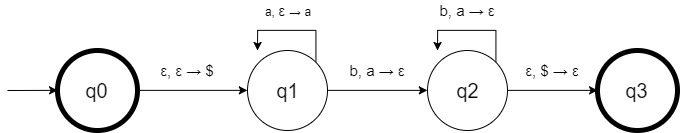
\includegraphics[scale=0.5]{p1}
	\end{figure}
	Diamo degli esempi di computazione:
	\begin{description}
		\item $(q_0, a^2b^2, \varepsilon) \Rightarrow (q_0, a^2b^2, \$) \Rightarrow (q_1, ab^2, a\$) \Rightarrow (q_1, b^2, a^2\$) \Rightarrow (q_2, b, a\$) \Rightarrow (q_2, \varepsilon, \$) \Rightarrow (q_3, \varepsilon, \varepsilon)$ \newline
	La parola viene correttamente accettata perché $q_3$ è finale e l'input è terminato. Notare che è ininfuente il fatto che la pila sia vuota ai fini dell'accettazione di una parola.
		\item $(q_0, a^4b^3, \varepsilon) \Rightarrow^{\star} (q_2, \varepsilon, a\$)$. La parola non viene accettata poiché $q_2$ non è finale.
		\item $(q_0, ab^2, \varepsilon) \Rightarrow^{\star} (q_3, b, \varepsilon)$. La parola non viene accettata poiché l'input non è stato completamente consumato.
	\end{description}
	\item \textit{Esempio 2:} Costruiamo $A \in PDA$ t.c. $L(A) =\{ a^nb^mc^{n-m} | n \geq m \geq 0\}$.
	\begin{figure}[H]
	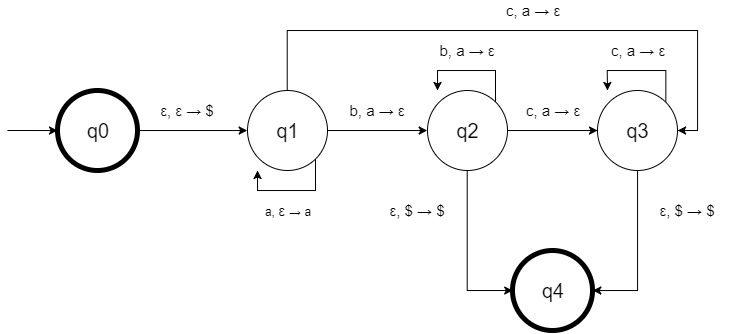
\includegraphics[scale=0.5]{p2}
	\end{figure}
	\item \textit{Esempio 3:} Costruiamo $A \in PDA$ t.c. $L(A) =\{ a^nb^{2n} | n \geq 0\}$.
	\begin{figure}[H]
	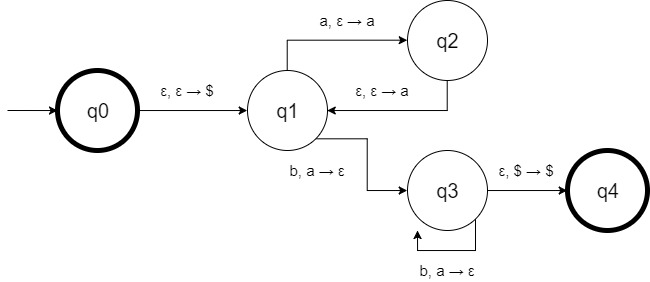
\includegraphics[scale=0.5]{p3}
	\end{figure}
\end{description}
\paragraph{Esercizi}
\begin{description}
	\item \textit{Esercizio 1:} Costruire $A \in PDA$ t.c. $L(A) =\{ a^nb^m | 0 \leq n \leq m \leq 2n \}$.
	\begin{figure}[H]
	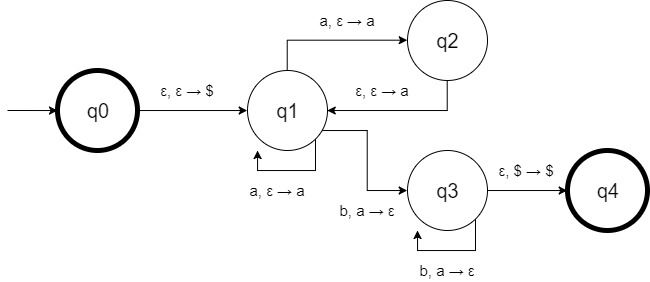
\includegraphics[scale=0.5]{p4}
	\end{figure}
	\item \textit{Esercizio 2:} Data la grammatica $G = ({S}, {0,1}, {S \to SS | 0S1 | 1S0 | \varepsilon}, S)$ fornire la descrizione del linguaggio che $G$ descrive.\newline
	\textit{Soluzione} $L = \{ x^n | n \geq 0 \land x \in \{0,1\}^{\star} \land n_1(x)=n_0(x)\}$, ossia un linguaggio formato da tutte parole che possono essere scomposte in sottostringhe tutte uguali in cui il numero di 1 è uguale al numero di 0.
	\item \textit{Esercizio 3:}  Data la grammatica $G = ({S, A}, {0,1}, {S \to AS | 0S1 | A, A \to 0A | 0 }, S)$ fornire la descrizione del linguaggio che $G$ descrive.\newline
	\textit{Soluzione:} $L = \{0^{n+k} 1^n | n \geq 0 \land k \geq 1\}$
	\item \textit{Esercizio 4:} Esprimere la grammatica dell'esercizio 2 in forma normale di Chomsky.\newline
	\textit{Soluzione:} Per essere sintetici scriveremo solo come vengono modificate le regole.
	\begin{enumerate}
		\setcounter{enumi}{0}
		\item \[S_0 \to S\] \[S \to SS | 0S1 | 1S0 | \varepsilon \]
		\item $NULL=\{S\}$
		\[S_0 \to S\] \[S \to SS | 0S1 | 01 | 1S0 | 10 \]
		\item $UNIT = \{(S_0, S_0),(S,S),(S_0, S)\}$
		\[S_0 \to  SS | 0S1 | 01 | 1S0 | 10 \] \[S \to SS | 0S1 | 01 | 1S0 | 10 \]
		\item $PROD = V$ e $DER = V$ quindi non dobbiamo fare modifiche.
		\item Aggiungiamo le regole per i terminali:
		\[A \to 0\]\[B \to 1\]
		\[S_0 \to  SS | ASB | AB | BSA | BA \] \[S \to SS | ASB | AB | BSA | BA \]
		Scomponiamo le regole in modo che la parte destra sia sempre di due variabili.
		\[A \to 0\]\[B \to 1\]\[C \to SB\]\[D \to SA\]
		\[S_0 \to  SS | AC | AB | BD | BA \] \[S \to SS |AC | AB | BD | BA \]
	\end{enumerate}
\end{description}

\newpage
%!TEX root=../../root.tex

\section{Lezione 12}
\subsection{PDA e DPDA}
\subparagraph{Esempi} Siano $L_1$ e $L_2$ i seguenti linguaggi:
\begin{description}
	\item $L_1 = \{ w\#w^R | w \in \{0,1\}^{\star}\}$, ossia l'insieme delle parole palindrome con un $\#$ al centro. \\
	\begin{figure}[H]
		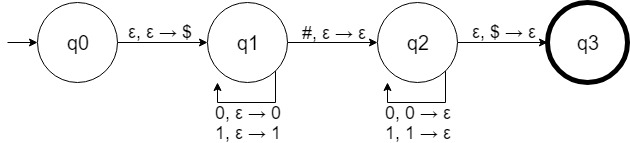
\includegraphics[scale=0.5]{pda1}
	\end{figure}
	\item $L_2 = \{ ww^R | w \in \{0,1\}^{\star}\}$, ossia l'insieme delle parole palindrome di lunghezza pari. \\
	\begin{figure}[H]
		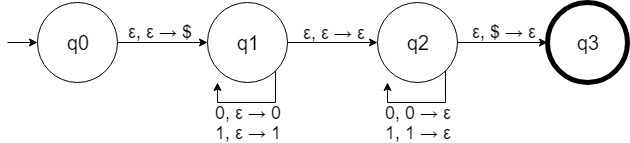
\includegraphics[scale=0.5]{pda2}
	\end{figure}
\end{description}
Nel linguaggio $L_1$ sappiamo quando abbiamo finito di leggere $w$ appena leggiamo $\#$ in input. A questo punto abbiamo $w$ impilata nella pila dell'automa e possiamo controllare che il resto dell'input sia esattamente $w$ al contrario.\\
Nel linguaggio $L_2$ invece non sappiamo con certezza quale sia il carattere che determina la fine della parola $w$ per tale motivo dobbiamo ricorrere al non determinismo. Infatti l'automa ha sempre la possibilit\`a di fare o non fare la $\varepsilon$ mossa. Quindi in $q_1$ ho sempre due possibilit\`a: continuare ad impilare oppure iniziare a togliere dalla pila. \\
Nei PDA il modello non deterministico è molto più potente dell'equivalente deterministico, infatti abbiamo che: 
\[ 
	L(DPDA) \subsetneq L(PDA)
\]
Questo è l'unico modello in cui questo è vero.\\
\textit{Dimostrazione:}
Dato un automa a pila deterministico $A = (Q,\Sigma,\Gamma,\delta,q_{0},F)$ la cui funzione di transizione è definita come segue:
\[
	\delta: Q\times \Sigma_{\varepsilon}\times\Gamma_{\varepsilon} \to {\cal P} (Q\times \Gamma_{\varepsilon})
\]
Affinch\'e A sia deterministico deve valere che:
\begin{enumerate}
	\item $|\delta(q,a,A)| \leq 1 \quad \forall  a \in \Sigma_{\varepsilon}, \forall A \in \Gamma_{\varepsilon}$
	\item $|\delta(q,\varepsilon,A)| = 1 \Rightarrow  \delta(q,a,A) = \emptyset \quad \forall  a \in \Sigma, \ \forall A \in \Gamma_{\varepsilon}$, ossia se da $q$ leggendo in input $\varepsilon$ e sulla cima della pila $A$ l'automa effettua una transizione allora da $q$ leggendo $A$ dalla pila e qualsiasi altro carattere in input l'automa non deve effettuare transizioni.
	\item $|\delta(q,a,\varepsilon)| = 1 \Rightarrow  \delta(q,a,A) = \emptyset \quad \forall  a \in \Sigma_{\varepsilon}, \ \forall A \in \Gamma$, ossia se da $q$ leggendo $a$ in input e la parola vuota dalla cima della pila l'automa effettua una transizione allora se in cima alla pila c'è un carattere diverso da $\varepsilon$ allora l'automa non deve effettuare transizioni.
\end{enumerate}

\subsection{Equivalenza tra linguaggi generati da PDA e CFL}
Si vuole dimostrare che $L(PDA) \textbf{=} L(CFG) = CFL$. 
\begin{enumerate}
	\item $L(PDA) \subseteq CFL$, non sar\`a trattata in questo documento.
	\item $CFL \subseteq L(PDA)$, utile dimostrazione poich\'e usa la stessa tecnica per costruire i parser di linguaggi di programmazione. \\
		Quindi vogliamo dimostrare che: $L \in L(CFL) \Rightarrow L \in L(PDA)$
\end{enumerate} 
\textit{Dimostrazione:}
Se $L \in L(CFL)$ allora $\exists \ G = \ (V,\Sigma,R,S) \ | \ L(G) \ = \ L $. Il seguente $PDA$ è costruito in modo da accettare il linguaggio denotato dalla grammatica G, quindi accetta il linguaggio $L$.
\begin{figure}[H]
	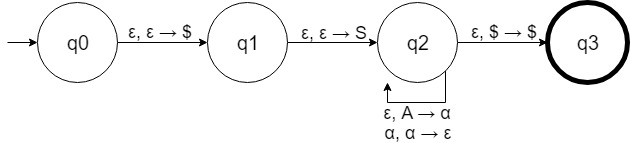
\includegraphics[scale=0.5]{pda3}
\end{figure}
\begin{description}
	\item \textit{Esempio:} Data la grammatica $G = (\{S,A\}, \{a, b\}, \{S \to aSA | \varepsilon, A \to bA | b\}, S )$ costruiamo il $PDA$ che riconosce il linguaggio descritto da $G$. \\
% Immagine		
\end{description}

\newpage 

\subsection{Modello di Turing}
Una macchina di Turing è caratterizzata da:
\begin{itemize}
	\item Un nastro di input con lunghezza infinita a destra, formato da celle che possono memorizzare un carattere l'una. Tra i caratteri vi è un carattere speciale utilizzato per indicare la cella vuota, detto blank, indicato con "B".
	\item Una testina per la lettura e la scrittura di caratteri sul nastro, la quale si pu\`o muovere sia a destra che a sinistra o restare ferma.
	\item Un insieme finito di stati in cui pu\`o transitare, fra cui uno stato iniziale $q_0$, lo stato di accettazione $q_a$ e lo stato di rifiuto $q_r$
\end{itemize}
\paragraph{Modello Formale} Sia M una macchina di Turing, essa è definita come la seguente 7-tupla
\[
	M = (Q,\Sigma,\Gamma,\delta,q_0,q_a,q_r) 
\]
Dove:
\begin{itemize}
	\item Q: insieme finito di stati di M
	\item $\Sigma \subseteq \Gamma$: alfabeto finito di input 
	\item $\Gamma$: alfabeto finito di nastro
	\item $\delta: Q\times\Gamma \to Q \times \Gamma \times\{L,R\}$: funzione di transizione
\end{itemize}
Anche in questo modello possiamo definire il concetto di \textit{configurazione}. Una configurazione deve mantenere le seguenti informazioni:
\begin{itemize}
	\item stato attuale 
	\item contenuto del nastro $\alpha \in \Gamma^{\star}$
	\item posizione della testina sul nastro
\end{itemize}
Sia $c$ una configurazione generica 
$$
c = \alpha p a \beta \text{ con }\alpha, \beta \in \Gamma^{\star} \ a \in \Gamma,  p \in Q
$$
essa ci fornisce le seguenti informazioni:
\begin{itemize}
	\item la macchina si trova sullo stato $p$
	\item il contenuto del nastro è $\alpha a \beta$
	\item la testina è posizionata sulla cella di $a$ (il primo carattere dopo lo stato)
\end{itemize}
Per descrivere un passo di calcolo abbiamo bisogno di definire una relazione ($\Rightarrow_M$) tra due configurazioni. Sia $c' = \alpha b q \beta$ un'altra configurazione dove $\alpha$ e $\beta$ sono le stesse di $c$, mentre $b \in \Gamma$ e $q \in Q$ potrebbero essere differenti. Le due configurazioni sono in relazione se da $c$ con un passo di calcolo si può raggiungere $c'$:
\[
	\text{Se }\delta(p,a) = (q, b, R) \text{ allora scriviamo } \alpha p a \beta \Rightarrow_M \alpha b q \beta \text{ ossia }  c \Rightarrow_M c' 
\]
Quindi dallo stato $p$ leggendo $a$ sul nastro viene scritto $b$ al posto di $a$ e viene fatto un passo a destra spostando la testina sul primo carattere di $\beta$ (non necessario esplicitarlo) e l'automa transita nello stato $q$.

Come al solito definiamo anche la chiusura riflessiva e transitiva di $\Rightarrow_M$ che ci aiuta nella definizione del linguaggio accettato dalla macchina $M$.
\[
	L(M) = \{ x \ | \ x \in \Sigma^{\star} \land q_0 x \Rightarrow_M^{\star} \alpha q_a\beta \text{ con } \alpha, \beta \in \Gamma^{\star}\}
\]
\subsection{Correlazione tra problemi di decisione e di ricerca}
Un \textit{problema di decisione} è un problema che risponde in modo dicotomico ad una certa domanda. Ad esempio dato un grafo stabilire se esiste un cammino aciclico. Invece un \textit{problema di ricerca} è un problema che trova un' istanza che soddisfi una certa domanda. Ad esempio dato un grafo esibire un cammino aciclico.

Vediamo ora il problema della ricerca di un assegnamento per una formula booleana che la renda soddisfatta. Partiamo dal problema di decisione correlato, ossia stabilire se esiste un assegnamento che renda soddisfatta la formula.
\\

\textbf{ALGSAT:}
\begin{description}
	\item \textit{Input:} $\varphi$, formula booleana
	\item \textit{Output:} "s\`i" se $\varphi$ è soddisfacibile, "no" altrimenti.
	\item \textit{Algoritmo:} ricerca esaustiva di un assegnamento. Nel caso peggiore se $\varphi$ è formata da $k$ variabili allora verranno generate $2^k$ stringhe binarie da testare.
\end{description}
Ora definiamo un algoritmo di ricerca che utilizza \textit{ALGSAT}:
\\

\textbf{ALGRICSAT:}
\begin{description}
	\item \textit{Input:} $\varphi$, formula booleana
	\item \textit{Output:} un assegnamento che soddisfa $\varphi$ se esiste, altrimenti "no".
	\item \textit{Algoritmo:}
		\begin{enumerate}
			\item esegui \textit{ALGSAT}. Se risponde "no" allora termina e rispondi "no", altrimenti continua.
			\item Si assegna 0 alla prima variabile e si esegue \textit{ALGSAT} sulla formula ottenuta $\varphi_0$. Se $\varphi_0$ non e' soddisfacibile si pone la prima variabile a 1.
			\item In entrambi i casi si prosegue nello stesso modo per la successive variabili.
			 
		\end{enumerate}
\end{description}

\newpage
%!TEX root=../../root.tex

\section{Lezione 13}
\subsection{Problemi di decisione}

Un problema può essere visto come l'insieme delle sue istanze, partizionate fra istanze sì e istanze no.
La tesi di Church-Turing afferma che la classe dei linguaggi riconosciuti da una TM corrisponde alla classe dei problemi effettivamente risolvibili. Quindi si può identificare l'idea di algoritmo con quella di una TM che si ferma sempre, mentre un semialgoritmo corrisponde ad una TM che non sempre si ferma.


\subsection{Semi-algoritmo per DFA vuoto}

input: $A = (Q,\Sigma,\delta,q_0,F)$ \\
output: sì se $L(A) \neq \emptyset$ \\
\begin{enumerate}
	\item Poni $x=\varepsilon$
	\item Esegui \emph{A} su \emph{x}
	\item Se \emph{A} accetta \emph{x} rispondi sì
	\item Altrimenti metti in \emph{x} la parola successiva nell'ordine canonico e torna a 2. 
\end{enumerate}

\subsection{Linguaggi non CFL}

\[
	L = \{ \ 0^{2^n} \ | \ n \geq 0 \ \}
\]

\emph{Algoritmo:}
\begin{enumerate}
	\item Sostituisci $B$ con il primo 0 sul nastro
	\item Spostare la testina verso destra sostituendo con \emph{x} ogni secondo 0
	\item Se il nastro non ha altri 0 $\rightarrow$ accetta
	\item Se num(0) è dispari $\rightarrow$ rifiuta
	\item Riporta la testina all'inizio del nastro e torna al punto 2
\end{enumerate}

\begin{figure}[H]
	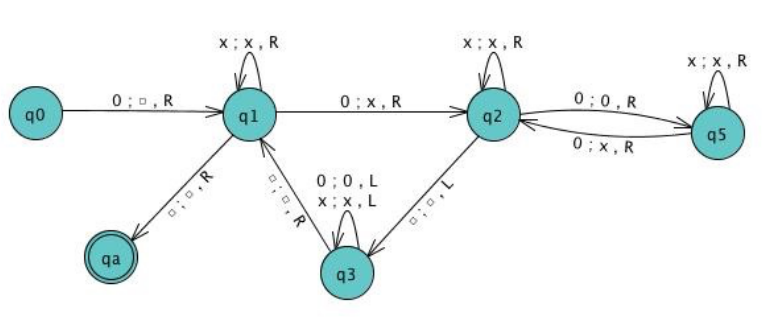
\includegraphics[scale=0.6]{TM1}
\end{figure}


\[
	L = \{ \ a^{n}b^{n}c^{n} \ | \ n \geq 0 \ \}
\]
\newpage
%!TEX root=../../root.tex

\section{Lezione 14}
\subsection{Macchine di Turing e Teoremi}
\subsubsection{Classe dei linguaggi Turing-Riconoscibili}
\[
	L(TM) = \{ L \ | \ \exists \ T \in TM \land L(T) = L \}
\]
\subsubsection{Classe dei linguaggi Turing-Decidibili}
\[
	L(TM_d) = \{ L \ | \ \exists \ T \in TM \land L(T) = L \land T \text{ si ferma sempre}\}
\]
\subsubsection{Equivalenza tra $TM$ a k nastri e TM} 
Una macchina di Turing a $k$ nastri è identica ad una "normale", a differenza della funzione di transizione, adattata per leggere, scrivere e muovere la testina per ognuno dei $k$ nastri. Essa è descritta formalmente così:
\[
	\delta: Q \times \Gamma^k \to Q \times (\Gamma \times \{ L, R \})^k
\]
\[
	\delta(q, a_1,a_2,...,a_k) = (p, (b_1,L), (b_2,R), ..., (b_k, L))
\]
che significa che se la macchina sta nello stato $q$ e legge $a_i$ sull'i-esimo nastro, va nello stato $p$ e sull'i-esimo nastro scrive $b_i$ e sposta la testina a destra o a sinistra.

Sia $L(TM_k)$ la classe dei linguaggi riconosciuti dalle macchine di Turing a $k$ nastri, vogliamo dimostrare che è equivalente ad $L(TM)$ e quindi che la versione a $k$ nastri delle macchine di Turing non \`e un modello pi\`u potente.


\textit{Dimostrazione:} Per dimostrare che $L(TM_k) = L(TM)$ dobbiamo dimostrare le due inclusioni $L(TM) \subseteq L(TM_k)$ e $L(TM_k) \subseteq L(TM)$.
\begin{itemize}
	\item $L(TM) \subseteq L(TM_k)$, questa inclusione è banale poiché le macchine di Turing a $k$ nastri con $k = 1$ sono le classiche macchine di Turing.
	\item $L(TM_k) \subseteq L(TM)$, per dimostrare questa inclusione utilizziamo il seguente teorema.
\end{itemize}
\subsubsection{Teorema}
\[
	T \in TM_k \Rightarrow \exists T' \in TM \land L(T) = L(T')
\] 
\textit{Dimostrazione:} Data $T \in TM_k$ vogliamo mostrare che possiamo costruire una macchina $T'$ con un unico nastro equivalente a $T$. $T'$ avrà il contenuto dei k nastri di $T$ sul suo unico nastro con dei delimitatori ($\#$) per riconoscere la fine del contenuto di un singolo nastro.
	\begin{itemize}
		\item \textit{Configurazione iniziale:} Sia $c_0^T$ la configurazione iniziale di $T$. Poiché $T$ ha $k$ nastri essa deve mantenere l'informazione sullo stato (lo stesso per tutti i $k$ nastri) e le celle di tutti i $k$ nastri, che sono tutti vuoti tranne il primo, il quale contiene l'input. 
		
		Quindi la configurazione iniziale è della forma
		$$c_0^T = (q_0 a_1...a_n, \  q_0B, q_0B, ...,\  q_0B)$$
		Con una serie di passi possiamo portare $T'$ in una configurazione iniziale equivalente:
		$$c_0^{T'} = (p_0 a_1...a_n) \Rightarrow^* (p(q_0) \ \dot{a_1}...a_n \ \# \dot{B} \# ... \# \ \dot{B} \#\#)$$
		dove il punto sopra un simbolo del nastro significa che la testina dell'$i$-esimo nastro di $T$ che stiamo simulando sta su quel simbolo, mentre $p(q_0)$ significa che $T'$ sta in uno stato equivalente a $q_0$ di $T$.
		\item \textit{Configurazione generica:} Assumiamo ora che $T'$ sia in una configurazione
		\[
			c = (p(q)\ \alpha_1 b_1 \dot{c}_1 d_1 \beta_1 \  \# ... \# \ \alpha_k b_k \dot{c}_k d_k \beta_k \ \#\#)
		\]
		e che la funzione di transizione di $T$ sia della forma
		\[
			\delta(q, c_1, ..., c_k) = (q', (f_1, L), ..., (f_k, R))
		\]
		Allora in una serie di passi possiamo portare $T'$ in una configurazione $c'$ in cui lo stato è cambiato seconda la funzione, mentre il nastro è rimasto invariato:
		$$c \Rightarrow^* c' = (p(q, c_1...c_k) \ \alpha_1 b_1 \dot{c}_1 d_1 \beta_1 \ \# ... \# \  \alpha_k b_k \dot{c}_k d_k \beta_k \ \#\#)$$
		Da questa configurazione possiamo poi cambiare le $k$ "posizioni di lettura" sul nastro, sempre simulando la funzione di transizione, arrivando ad una configurazione $c''$:
		\[
			c' \Rightarrow^* c'' = (p(q') \ \alpha_1 \dot{b_1} f_1 d_1 \beta_1 \ \# ... \# \  \alpha_k b_k f_k \dot{d_k} \beta_k \ \#\#)
		\] 
		
		\item \textit{Configurazione di accettazione}:
		La macchina $T'$ deve accettare quando la macchina $T$ che sta simulando arriva in $q_a$, ovvero quando raggiunge una configurazione
		$$
		c = (p(q_a) \ \alpha_1 \dot{c_1} \beta_1  \# ... \# \  \alpha_k \dot{c_k} \beta_k \ \#\#)
		$$ 
	\end{itemize}
\subsubsection{NTM, macchine di Turing non deterministiche} Ridefiniamo la funzione di transizione per le macchine di Turing non deterministiche. 
\[
	\delta : Q \times \Gamma \to {\cal P} (Q \times (\Gamma \times \{L, R\} ))
\]
Per rendere la funzione totale aggiungiamo:
\[
	\delta(q_a, a) = \emptyset,\ \delta(q_r, a) = \emptyset\ \ \ \forall a \in \Gamma
\]

Partendo da una configurazione iniziale possiamo ricavare l'albero delle computazioni di una $NTM$. Questo albero può non essere finito in quanto non abbiamo certezza che la macchina si fermi. 

Definiamo \textit{grado di non determinismo} di un nodo il numero di figli che esso ha nell'albero, ovvero il numero di possibili configurazioni in cui la $NTM$ può andare da una certa configurazione.

Sia $d$ il massimo grado di non determinismo di un albero $$d = max\{ |\delta(q, a)| \ | \ q \in Q, \ a \in \Gamma  \}$$
 allora ogni nodo ha al massimo $d$ figli e quindi l'albero è $d$-ario, non necessariamente completo.

Sulla base dell'albero possiamo definire la condizione di accettazione e di rifiuto:

\begin{itemize}
 \item \textit{Condizione di accettazione}: L'albero ha almeno un ramo finito, che quindi termina in una foglia, e tale foglia è una configurazione di accettazione
 
 \item \textit{Condizione di rifiuto}: L'albero è \textbf{finito}, e ogni foglia è una configurazione di rifiuto o bloccata. 
 \end{itemize} 

Da ciò discende che è molto più facile stabilire se un input viene accettato piuttosto che rifiutato. Se abbiamo un albero senza nessuna foglia allora vuol dire che la macchina su quell'input non termina mai, ma non possiamo concludere che l'input venga rifiutato, possiamo solo dire che non è accettato.

\subsubsection{Teorema: equivalenza tra TM e NTM}

Il non determinismo non aumenta il potere della macchina di Turing: mostriamo che è possibile costruire una $TM$ che simula una $NTM$.

L'idea è "visitare" l'albero, simulando tutti i possibili rami di computazione. La visita avviene per livelli in quanto andare in profondità potrebbe portarci ad esplorare rami infiniti prima di rami che portano a configurazioni di accettazione o di rifiuto.

Ogni nodo dell'albero è univocamente determinato dalla sequenza di scelte che dalla dalla radice portano al nodo. Per codificare le scelte numeriamo i figli di ogni nodo e diciamo che da una certa configurazione la macchina ha effettuato la scelta $i$ se passiamo alla configurazione corrispondente all' $i$-esimo figlio del nodo corrispondente.

Possiamo rappresentare tutti i possibili cammini sull'albero $d$-ario (che supponiamo essere completo) dalla radice ad un qualsiasi nodo come una stringa $s \in \{1, ..., d\}^*$. L'ordine canonico descrive la visita per livelli.
\\
\\

Diamo ora una descrizione di una $T' \in TM$ equivalente a una $T \in NTM$:
\begin{itemize}
	 \item $M_0 \in TM$ è usata per enumerare i cammini da simulare\\
	 \textit{input}: $x \in \{1, ..., d\}^*$ \\
	 \textit{descrizione}: rimpiazza $x$ con la stringa successiva nell'ordine canonico
	 
	 \item $T' \in TM$ simula $T$ tramite 3 nastri:
	 \begin{enumerate}
	 \item il primo nastro contiene la stringa di input di $T$
	 \item il secondo nastro è il nastro di lavoro
	 \item il terzo nastro contiene la codifica del ramo di computazione che sta simulando
	 \end{enumerate}
	 \textit{input}: $s \in \Sigma^*$\\
	 \textit{descrizione}:
	 \begin{enumerate}
	 \item inizializza il terzo nastro con 1 (la configurazione iniziale)
	 
	 \item copia l'input $s$ sul nastro di lavoro ed esegui le mosse che $T$ fa (se ce ne sono) per raggiungere la configurazione identificata dalla stringa sul terzo nastro.
	 \begin{itemize}
	 \item se si raggiunge $q_a$, accetta
	 
	 \item se manca una mossa o si raggiunge una configurazione di rifiuto esegui $M_0$ sulla stringa sul terzo nastro, cancella il secondo nastro e ricomincia il punto 2
	 \end{itemize}
	 \end{enumerate}
 \end{itemize} 

\newpage
%!TEX root=../../root.tex

\section{Lezione 15}
\subsection{Problema dell'appartenenza per TM}
Chiameremo il problema dell'appartenenza per macchine di Turing $A_{TM}$. Questo è anche primo esempio di macchina universale, in pratica un calcolatore. Questa macchina prende in input un' altra macchina e un suo input e il risultato della computazione dipende dal risultato dell'esecuzione della macchina presa in input sul suo input.
\[
	A_{TM} = \{ <T, x> | x \in L(T)\}
\]
$A_{TM}$ è Turing-Riconoscibile ma non decidibile.
[immagine dei Problemi di decisione che includono i Turing-riconoscibili, che includono i decidibili]
\subsection{Teorema}
\[
	A_{TM}\ non\ decidibile
\]
\textit{Dimostrazione:} Supponiamo per assurdo che $A_{TM}$ sia decidibile $\Rightarrow \exists T \in TM \quad t.c. \quad L(T)=A_{TM}$ e si ferma sempre \\
\begin{equation*}
	T(<M,w>) =
	\begin{cases}
   	accetta \ se \ M \ accetta \ w\\rifiuta \ altrimenti
   	\end{cases}
\end{equation*}
Considero la macchina T' uguale a T ma con le uscite invertite:
\begin{equation*}
	T'(<M,w>) =
	\begin{cases}
   	accetta \ se \ w \notin L(M)\\rifiuta \ se \ w \in L(M)
   	\end{cases}
\end{equation*}
Considero T'' che si comporta come T' ma prende in input due codifiche di macchine

\begin{equation*}
	T''(<M,<M'>>) =
	\begin{cases}
   	accetta \ se \ <M'> \notin L(M)\\rifiuta \ se \ <M'> \in L(M)
   	\end{cases}
\end{equation*}

\begin{tabular}[left]{ c | c c c c }
	T'' & $<M1>$ & $<M2>$ & $<M3>$ & $\cdots$ \\
	\hline
	M1 & acc & rif & acc & $\cdots$ \\
	M2 & rif & rif & acc & $\cdots$ \\
	M3 & acc & acc & rif & $\cdots$ \\
	$\vdots$ & $\vdots$ & $\vdots$ & $\vdots$ & $\vdots$ 
\end{tabular} \\ \\
Descriviamo ora la diagonale della macchina T'' con una macchina T'''
\begin{equation*}
	T'''(<M>) =
	\begin{cases}
   	accetta \ se \ <M> \notin L(M)\\rifiuta \ se \ <M> \in L(M)
   	\end{cases}
\end{equation*}
Tra le macchine M, posso considerare anche T''', per cui T''' diventa:
\begin{equation*}
	T'''(<T'''>) =
	\begin{cases}
   	accetta \ se \ <T'''> \notin L(T''')\\rifiuta \ se \ <T'''> \in L(T''')
   	\end{cases}
\end{equation*}
Qui arriviamo a una contraddizione, poiché T''' ci dice che:
\begin{center}
	$<T'''> \in L(T''') \Leftrightarrow <T'''> \notin L(T''')$ \footnote{Paradosso di Russel: Siano F = $\{X \mid X \text{ è infinito}\}$, E = $\{X \mid X \text{ è finito}\}$ e R = $\{X \mid X \notin X\}$. \\
	$F \in R? \text{ Si, poiché F è a sua volta un insieme infinito}$ \\
	$E \in R? \text{ No, perché E è un insieme infinito}$ \\
	$R \in R? \ R \in R \Rightarrow R \notin R, ma R \notin R \Rightarrow R \in R $ }
\end{center} 
\subsection{Teorema}
Se L è Turing-Riconoscibile e anche $\overline{L}$ lo è, allora L è decidibile \\
\textit{Dimostrazione:}
\[
	\exists T,T' \in TM \mid L(T)=L \ e \ L(T') = \overline{L}
\] 
\begin{figure}[H]
	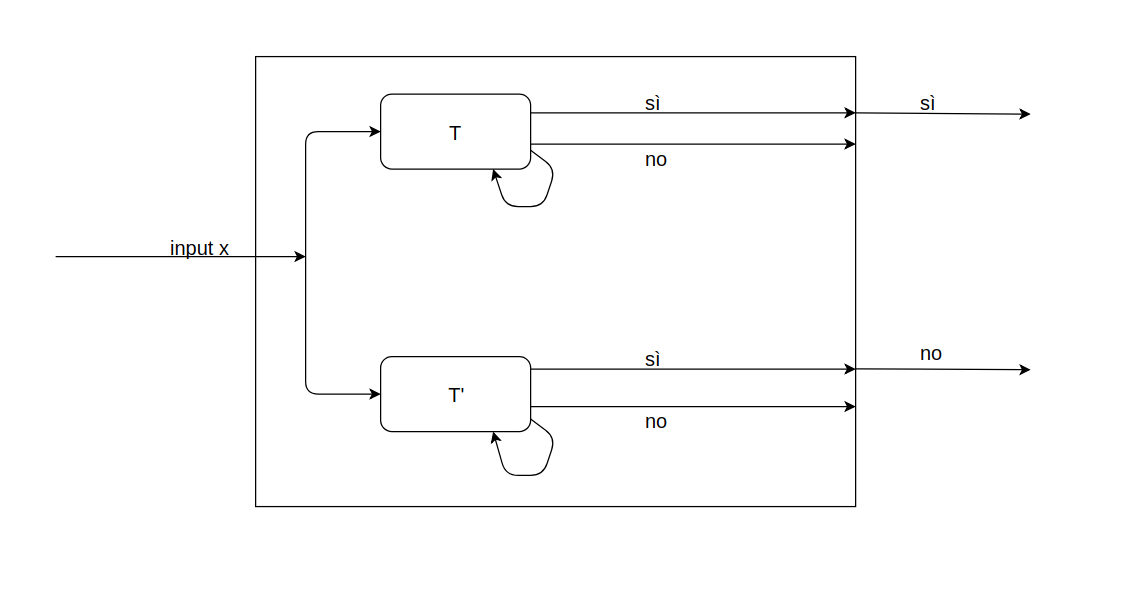
\includegraphics[scale=0.35]{automa-parallelo}
\end{figure}
Descrizione di M:
\begin{description}
	\item \textit{input}: x
	\item \textit{output}: s\`i se x $\in$ L, no altrimenti 
	\item \textit{Descrizione ad alto livello}:
		\begin{enumerate}
			\item fai una mossa di T sul primo nastro, se T accetta, allora accetta
			\item fai una mossa di T' sul secondo nastro, se T' accetta, allora rifiuta
		\end{enumerate}			
\end{description}

\subsubsection{Corollario}
\[
	\overline{A_{TM}}\ non\ \text{è}\ Turing-Riconoscibile
\]
\textit{Dimostrazione:} 
$A_{TM}$ è Turing-Riconoscibile e quindi se $\overline{A_{TM}}$ fosse Turing-Riconoscibile dovrei dedurre che $A_{TM}$ sia decidibile. \\
\\
$A_{TM} = \{ <M,w> \ \mid \ w \in L(M) \ e \ M \in TM \}$ \\
\\
$\overline{A_{TM}} = \{ X \mid \text{X non codifica M,w} \} \cup \{ <M,w> \mid M \in TM \text{ e } w \notin L(M) \}$
\subsection{Il problema della fermata}
$Halt_{TM} = \{ <M,w> \ e \ M \in \text{TM e M si ferma su w} \}$ \\
\textit{$Halt_{TM}$ non è decidibile} \\
\textit{Dimostrazione: } Per assurdo supponiamo che $Halt_{TM}$ sia decidibile
\begin{equation*}
	\exists T \in TM \text{ tale che } T(<M,w>) = 
	\begin{cases} 
		\text{accetta se M si ferma su w} \\ 
		\text{rifiuta se M non si ferma}
	\end{cases} 
\end{equation*}
T': 
\begin{description}
\item \textit{input}: $<M, w>$
\item \textit{output}: sì se $w \in L(M)$, no altrimenti
\item \textit{descrizione}:
\begin{enumerate}[label*=\arabic*.]
\item esegue $T$ su $<M,w>$

\item se $T$ accetta, allora $M$ si ferma su $w$, quindi:

\begin{enumerate}[label*=\arabic*.]

\item esegue $M$ su $w$

\item se $M$ accetta $w$, allora accetta $<M,w>$

\item se $M$ rifiuta $w$, allora rifiuta

\end{enumerate}

\item se $T$ non accetta $<M,w>$ allora rifiuta

\end{enumerate}
\end{description}

Quindi per ogni codifica di macchina e input $<M, w>$ abbiamo che:

\begin{gather*}
	<M,w> \ \in \ L(T') \ se \ w \in L(M)\\
	<M,w> \ \notin \ L(T') \ se \ w \notin L(M)
\end{gather*}
Ovvero $T'$ decide $A_{TM}$, sfruttando $T$, ma abbiamo dimostrato che $A_{TM}$ non è decidibile, quindi $T$ non può esistere [Contraddizione].

\subsection{Mapping Reduction}
\begin{figure}[H]
	\centering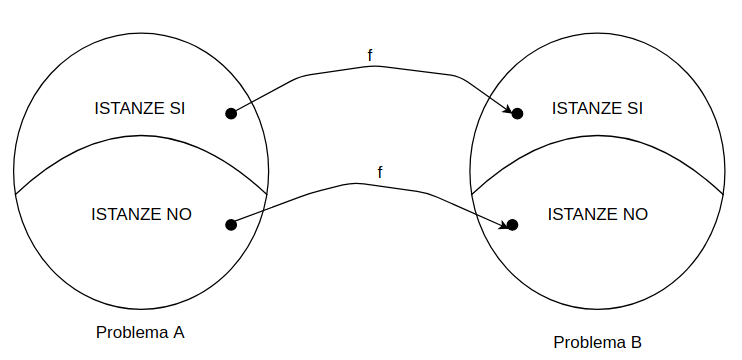
\includegraphics[scale=0.4]{riduzione}
\end{figure}
Siano $A,B \subseteq \Sigma^{\star}$ due problemi, con $A \le_{m} B$ si indica che il problema A "\textit{si riduce}" al problema B.
\begin{center}
	$A \le_{m} B \iff \exists f: \Sigma^{\star} \rightarrow \Sigma^{\star} \text{ tale che:}$
	\begin{enumerate}
		\item $f$ deve essere calcolabile ovvero $ \exists \ T_{f} \in TM \text{ t.c ricevendo } x \in \Sigma^{\star} \text{ in input scrive } $\\
$ f(x) \text{ sul nastro e si ferma}$ \\
		\item $x \in A \Leftrightarrow f(x) \in B$
	\end{enumerate}
\end{center}

\subsubsection{Teorema}

Se $A \le_{m} B$ e B è decidibile, allora $A$ è decidibile

\textit{Dimostrazione:} \\
$A \le_{m} B \Rightarrow \exists \text{f calcolabile x} \in A \Leftrightarrow f(x) \in B$
\begin{fleqn}
    \begin{align*}
		B \text{ è decidibile} \Rightarrow \exists T_{B} \in TM \ t.c. T_{B}(x) =
		\begin{cases}
			\text{accetta se x è in B} \\ \text{rifiuta altrimenti}
		\end{cases}
	\end{align*}
\end{fleqn}
Combino le due macchine:
\begin{figure}[H]
	\centering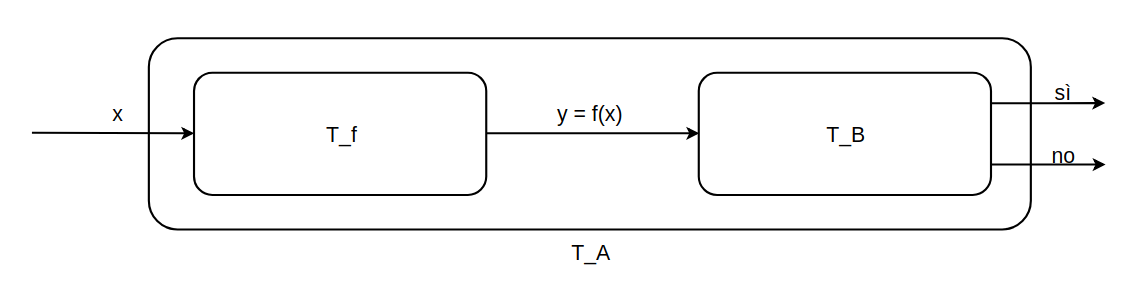
\includegraphics[scale=0.35]{automa-serie.png}
\end{figure}
\subsection{Teorema}

$A \le_{m} \text{B e supponiamo che A sia non decidibile, allora B non è decidibile}$ \\
\textit{Dimostrazione:}

Per assurdo se B fosse decidibile allora A sarebbe decidibile contro l'ipotesi \\
\\
\paragraph*{Esempio}
Sia $E_{TM}$ il linguaggio delle codifiche delle macchine che riconosco almeno una parola. Più formalmente: 
\[
	E_{TM} = \{ \ <T>  \ \mid \ T  \in TM \land L(T) \not= \emptyset \ \}
\]
Dimostriamo che $E_{TM}$ non è decidibile per riduzione utilizzando il seguente teorema: dato $A$ non decidibile se $A \le_{m} B$ allora $B$ non è decidibile.\\
Quindi se riduciamo $A_{TM}$ ad $E_{TM}$ abbiamo dimostrato che $E_{TM}$ non è decidibile poiché $A_{TM}$ non è decidibile.\\
Definiamo una macchina che calcola la funzione di riduzione di cui abbiamo bisogno. Questa macchina prende in input lo stesso input di $A_{TM}$, ossia la codifica di una macchina $M$ e di un suo input $w$ e fornisce in output la codifica di un' altra macchina $T$.
\[
	<M,w> \ \xrightarrow{f} \ <T>
\]
Sia $R_f$ la macchina che calcola la funzione di riduzione. Essa è costruita nel seguente modo:
\begin{description}
	\item \textit{Input:} $<M,w>$
	\item \textit{Output:} $<T>$
	\item \textit{Descrizione:} costruisce T come descritto di seguito.
\end{description}
T:
\begin{description}
	\item \textit{Input:} $x \in \Sigma^{\star}$
	\item \textit{Output:} s\`i se $w \in L(M) \Rightarrow L(T) = \Sigma^{\star}$, no se $w \notin L(M) \Rightarrow$ (w è rifiutata da M o M non si ferma)
	\item \textit{Descrizione:}
	\begin{enumerate}
		\item Esegui M su w
		\item Se M accetta w $\rightarrow$ accetta x
		\item Se M rifiuta w $\rightarrow$ rifiuta x
	\end{enumerate}
	\item \textit{Correttezza:}
		\item Se $w \in L(M)$ allora $L(T) = \Sigma^{\star}$, poiché $T\ \forall x \in \Sigma^{\star}$ accetta $x$ e quindi $E_{TM}$ risponderà sì.
		\item Se $w \notin L(M)$ allora $
			\begin{cases}
				\text{w è rifiutata da M} \\ \text{M non si ferma su w}
			\end{cases}
			\rightarrow L(T) = \emptyset \text{ e quindi } E_{TM} \text{ risponderà no }$
\end{description}
Quindi abbiamo ridotto $A_{TM}$ ad $E_{TM}$ con l'uso della funzione di riduzione $R_f$.

\newpage
%!TEX root=../../root.tex

\section{Lezione 16}

\subsection{Indecidibilità di $Halt_{TM}$ tramite riduzione}

In alternativa alla dimostrazione "tradizionale", mostriamo che si può mostrare la non decidibilità di $Halt_{TM}$ riducendo $A_{TM}$, che sappiamo essere indecidibile, ad esso:
$$A_{TM} \leq_{m} Halt_{TM}$$
Dobbiamo quindi esibire una $f: \Sigma^{\star} \to \Sigma^{\star}$ che mappa istanze sì di $A_{TM}$ in istanze sì di $Halt_{TM}$ e istanze no in istanze no. Ricordiamo che 
\begin{gather*}
A_{TM} = \{ <M, w> \ | \ T \in TM \land w \in L(M) \} \\
Halt_{TM} = \{ <T, w> \ | \ T \in TM \land M \text{ si ferma su } w \}
\end{gather*}
Quindi la funzione di riduzione $f$ dovrà comportarsi nel seguente modo:
\[
	<M, w> \mapsto <T, w> \text{ tale che } M \text{ accetta } w \iff T \text{ si ferma su } w
\]
Diamo ora una descrizione di una macchina $R_f$ che calcola $f$:
\begin{description}
\item \textit{input}: $<M, w>$

\item \textit{output}: $<T, w>$, descriviamo ora la $T$ prodotta:

\begin{description}
\item \textit{input}: $x$

\item \textit{descrizione}: 
\begin{enumerate}
\item esegui $M$ su $w$
\item se $M$ accetta $w$ allora accetta $x$
\item se $M$ rifiuta $w$ allora "\textit{cicla}"
\end{enumerate}
\end{description}
\end{description}

\subparagraph{Prova di correttezza}
\begin{itemize}
\item Se $M$ accetta $w$, la macchina $T$ accetta $x$, e in particolare si ferma.

\item Se $M$ \textit{non} accetta $w$, abbiamo due casi:
\begin{enumerate}
\item se $M$ rifiuta $w$ allora $T$ "cicla", ovvero $R_f$ ha opportunamente realizzato $T$ in modo da non farla terminare in questo caso, quindi $T$ non si ferma

\item se $M$ non si ferma su $w$, a maggior ragione non si ferma $T$ che sta eseguendo $M$ su $w$
\end{enumerate}
Quindi in entrambi i casi $T$ non si ferma.
\end{itemize}
Abbiamo dunque costruito un decisore per $A_{TM}$, supponendo di avere un decisore per $Halt_{TM}$; tuttavia sappiamo che un decisore per $A_{TM}$ non può esistere, quindi necessariamente non può esistere un decisore per $Halt_{TM}$, ovvero esso è \textbf{indecidibile}.

\subsection{Esercizi sulle riduzioni}

\paragraph{TM che accettano linguaggi regolari}

\[
	REG_{TM} = \{ <T>\ | \ T \in TM \land L(T) \text{ è regolare} \}
\]

Mostriamo che è un linguaggio indecidibile riducendo $A_{TM}$ ad esso:
\[
	<M, w> \xmapsto{f} <T> \text{ tale che } M \text{ accetta } w \iff L(T) \text{ è regolare}
\]
Per procedere dobbiamo pensare a come costruire una macchina $T$ tale che $L(T)$ non è regolare sulle istanze no di $A_{TM}$, mentre lo è sulle istanze sì: qualsiasi coppia di linguaggio regolare e non regolare va bene, quindi per comodità scegliamo di costruire $T$ così che 
\begin{gather*}
L(T) = \Sigma^{\star} \text{ per le istanze sì di } A_{TM}\\
L(T) = 0^n1^n \text{ per le istanze no di } A_{TM}
\end{gather*}
Una utile proprietà di questa scelta è che $0^n1^n \subset \Sigma^{\star}$, per cui possiamo (definire $R_f$ in modo da) costruire $T$ in modo che accetti \textit{almeno} $0^n1^n$, indipendentemente dall'accettazione di $w$. Successivamente $T$ controllerà se $M$ accetta $w$ o meno: 
\begin{enumerate}
\item nel primo caso, accetterà anche tutti gli input $x$ \textit{non} della forma $0^n1^n$, ovvero il resto di $\Sigma^{\star}$, rendendo $L(T)$ regolare

\item nel secondo caso rifiuterà tutto il resto di $\Sigma^{\star}$, continuando ad accettare solo input $x$ della forma $0^n1^n$, quindi lasciando $L(T)$ non regolare
\end{enumerate} 

La funzione di riduzione $f$ è quindi così definita:
\begin{description}
\item \textit{input}: $<M, w>$
\item \textit{output}: $<T>$ dove $T \in TM$ è così definita:
\begin{description}
\item \textit{input}: $x$
\item \textit{descrizione}:
\begin{enumerate}
\item se $x = 0^n1^n$ per qualche $n \geq 0$, accetta $x$
\item altrimenti esegui $M$ su $w$
\item se $M$ accetta $w$, accetta $x$
\item se $M$ rifiuta $w$, rifiuta $x$

\end{enumerate}
\end{description}
\end{description}

\subparagraph{Prova di correttezza}

\begin{itemize}
\item Se $M$ accetta $w$, allora $L(T) = \{0^n1^n \ | \ n \geq 0\} \cup \neg \{0^n1^n \ | \ n \geq 0\} = \Sigma^{\star} \in REG$.

\item Se $M$ non accetta $w$, abbiamo due casi:
\begin{enumerate}
\item se $M$ rifiuta $w$, allora $L(T) = \{0^n1^n \ | \ n \geq 0\} \notin REG$
\item se $M$ non termina su $w$, allora non termina nemmeno $T$ che la esegue, per cui non accetta alcun $x$ che non sia della forma $0^n1^n$, perciò di nuovo $L(T) = \{ 0^n 1^n  \ | \ n \geq 0 \} \notin REG$
\end{enumerate}
Quindi in entrambi i casi $L(T) \notin REG$.
\end{itemize}

\paragraph{TM che accettano linguaggi $REV$}
\[
	REV_{TM} = \{ <T> \ | \ T \in TM \land w \in L(T) \implies w^{rev} \in L(T) \}
\]
Vogliamo costruire una $R_f$ che calcola una $f$ che riduca $A_{TM}$ a $REV_{TM}$ in modo da mostrarne l'indecidibilità. Come nell'esercizio precedente, ci scegliamo per comodità un linguaggio "semplice" che gode della proprietà desiderata, ad esempio $\{ 01, 10\}$ e uno che non ne gode, ad esempio $\{01\}$. 

Con questa scelta, di nuovo possiamo far sì che $R_f$ costruisca $T$ tale da accettare \textit{almeno} $x = 01$, ovvero $L(T) = \{01 \}$ che non gode della proprietà. 

Poi eseguendo $M$ su $w$ capirà se accettare anche $x = 10$, ovvero $L(T) = \{ 01, 10 \}$ che gode della proprietà, quindi $<T> \in REV_{TM}$, oppure no, lasciando $L(T)$ inalterato e quindi $<T> \notin REV_{TM}$.

Formalmente definiamo $R_f$ come una $TM$ che calcola $f$ nel seguente modo:
\begin{description}
\item \textit{input}: $<M, w>$
\item \textit{output}: $<T>$ dove $T \in TM$ è così definita:
\begin{description}
\item \textit{input}: $x$
\item \textit{descrizione}:
\begin{enumerate}
\item se $x = 01$, accetta $x$
\item altrimenti esegui $M$ su $w$
\item se $M$ accetta $w$ e $x = 10$, accetta $x$
\item se $M$ rifiuta $w$, oppure $x \neq 10$, rifiuta $x$

\end{enumerate}
\end{description}
\end{description}


\subparagraph{Prova di correttezza}

\begin{itemize}
\item Se $M$ accetta $w$, allora $L(T) = \{01 \} \cup \{ 10 \} = \{01, 10\} $ che rispetta la proprietà

\item se $M$ non accetta $w$, abbiamo due casi:
\begin{enumerate}
\item se $M$ rifiuta $w$, allora $L(T) = \{ 01 \}$ che non rispetta la proprietà
\item se $M$ non termina su $w$, allora non termina nemmeno $T$ che la esegue, per cui non accetta alcun $x$ che non sia $01$, perciò di nuovo $L(T) = \{ 01 \}$ che non rispetta la proprietà.
\end{enumerate}
Quindi in entrambi i casi $L(T) = \{01\}$ che non rispetta la proprietà.
\end{itemize}

\subsection{Dimostrare la non Turing-riconoscibilità di un linguaggio}

\paragraph{Teorema}
\[
	B \text{ è Turing-riconoscibile e } A \leq_m B \implies A \text{ è Turing-riconoscibile}
\]

\subparagraph{Prova}

Una $T_A \in TM$ che riconosce $A$ è molto semplice da costruire:
\begin{itemize}
\item \textit{input}: $x$
\item \textit{descrizione}:
\begin{enumerate}
\item esegui $R_f$
\item esegui $T_B$ su $f(x)$ prodotta da $R_f$
\end{enumerate}
\end{itemize}
Poiché $B$ è Turing-riconoscibile, per definizione esiste una $T_B$ tale che $L(T_B) = B$.\\
Poiché $f$ di riduzione deve essere calcolabile, per definizione esiste una $R_f$ che prende in input $x$ e restituisce in output sul nastro $f(x)$. Dunque $T_A$ così costruita è effettivamente una macchina di Turing corretta.

\begin{figure}[H]
	\centering 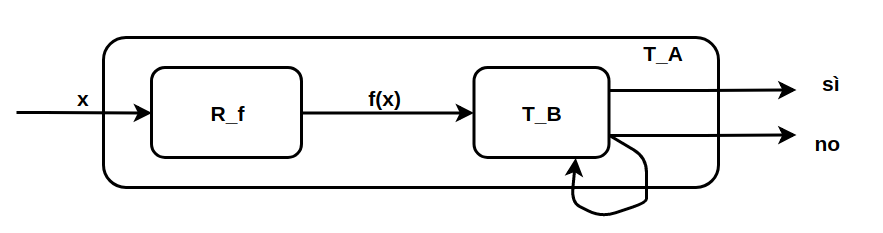
\includegraphics[scale=0.5]{teorema-1}
\end{figure}

\subparagraph{Corollario} $A \ \neg \text{Turing-riconoscibile e } A \leq_m B \implies B \ \neg \text{Turing-riconoscibile}$

\paragraph{Teorema}
\[
	A \leq_m B \iff \neg A \leq_m \neg B
\]
\subparagraph{Prova} Se $A \leq_m B$ allora deve esistere una qualche $f$ di riduzione per cui $\forall a \in A, \ b \in B \quad a \xmapsto{f} b$ (istanze sì) e $\forall x \notin A, \ y \notin B \quad x \xmapsto{f} y$ (istanze no).

Ma poiché le istanze sì di $\neg A$ sono le istanze no di $A$, e lo stesso vale per $B$, allora la $f$ è una funzione di riduzione anche per $\neg A$ e $\neg B$, in quanto:
\begin{enumerate}
 \item è ancora definita come $f: \Sigma^{\star} \to \Sigma^{\star}$
 \item è ancora calcolabile
 \item mappa ancora istanze sì ad istanze sì e istanze no ad istanze no
 \end{enumerate}
Abbiamo quindi esibito una funzione di riduzione di $\neg A$ a $\neg B$, perciò possiamo scrivere $\neg A \leq_m \neg B$.

Naturalmente per dimostrare l'altro verso della implicazione basta prendere $A' = \neg A$ e $B' = \neg B$ e applicare l'implicazione dimostrata precedentemente: \\
$A' \leq_m B' \implies \neg A' \leq_m \neg B'$ che è come dire $\neg A \leq_m \neg B \implies A \leq_m B$.

Quindi è vera la coimplicazione.

\subsection{Il problema dell'equivalenza $EQ_{TM}$}

Le istanze sì del problema sono costituite da tutte le codifiche di una coppia di macchine di Turing $T_1, T_2$\textit{equivalenti}, ovvero tali che $L(T_1) = L(T_2)$. 

\[
	EQ_{TM} = \{ <T_1, T_2> \ | \ T_1, T_2 \in TM \land L(T_1) = L(T_2)  \}
\]

Questo problema non solo è indecidibile, ma è anche non Turing-riconoscibile. Inoltre è l'unico problema che incontriamo nel corso per cui anche il complemento è non Turing-riconoscibile

\paragraph{Teorema} $EQ_{TM}$, il problema dell'equivalenza tra $TM$, non è Turing-riconoscibile

\subparagraph{Prova} Riduciamo $\neg A_{TM}$, che sappiamo essere non Turing-riconoscibile, a $EQ_{TM}$:
\[
	\neg A_{TM} \leq_m EQ_{TM}
\]
Tuttavia ridurre \textit{da} un problema non Turing-riconoscibile è complicato perché bisogna effettuare un mapping $<M, w> \xmapsto{f} <T_1, T_2>$che garantisce che $<T_1, T_2> \in L(EQ_{TM})$ non solo se $M$ rifiuta $w$, ma anche se $M$ non si ferma su $w$. Questa ultima condizione è chiaramente difficile da imporre.

Sfruttiamo allora il teorema di equivalenza tra riduzioni per portarci ad un caso più trattabile:
\[
	\neg A_{TM} \leq_m EQ_{TM} \text{ è come dire } A_{TM} \leq_m \neg EQ_{TM}
\]
Vogliamo quindi esibire una $f$ così definita:
\begin{gather*}
	f: \Sigma^{\star} \to \Sigma^{\star} \text{ calcolabile} \\
	<M, w> \xmapsto{f} <T_1, T_2> \text{ tale che } w \in L(M) \iff <T_1, T_2> \notin EQ_{TM}
\end{gather*}

L'idea è quindi fare sì che le $T_1, T_2$ costruite riconoscano lo stesso linguaggio se $w \notin L(M)$, mentre riconoscano due linguaggi diversi se $w \in L(M)$. Il modo più semplice di farlo è costruire $T_1$ in modo che non accetta mai nulla, ovvero tale che $L(T_1) = \varnothing$ sempre, mentre $T_2$ nel seguente modo:
\[
	\begin{cases}
		w \in L(M) \implies T_2 \text{ accetta qualsiasi x, ovvero } L(T_2) = \Sigma^{\star} \\
		w \notin L(M) \implies T_2 \text{ non accetta alcun x, ovvero } L(T_2) = \varnothing
	\end{cases}
\]
Quindi una $R_f$ che calcola $f$ ad alto livello è così definita:

\begin{description}
\item \textit{input}: $<M, w>$
\item \textit{output}: $<T_1, T_2>$ così definite:
\begin{itemize}
\item $T_1$:
\begin{description}
	\item \textit{input}: $x$
	\item \textit{descrizione}:
	\begin{enumerate}
	\item rifiuta $x$
	\end{enumerate}
\end{description}

\vspace{1cm}

\item $T_2$
\begin{description}
\item \textit{input}: $x$

\item \textit{descrizione}:
\begin{enumerate}
\item esegui $M$ su $w$
\item se $M$ accetta $w$ allora accetta $x$
\item se $M$ rifiuta $w$ allora rifiuta $x$
\end{enumerate}
\end{description}
\end{itemize}
\end{description}

\subparagraph{Prova di correttezza}

Vediamo se $R_f$ così costruita rispetta la proprietà voluta:

\begin{itemize}
\item se $M$ accetta $w$, allora $L(T_1) = \varnothing$ mentre $T_2$ accetta qualsiasi $x$, per cui $L(T_2) = \Sigma^{\star}$, di conseguenza $L(T_1) \neq L(T_2) \implies <T_1, T_2> \notin EQ_{TM}$.

\item se $M$ \textit{non} accetta $w$, allora abbiamo due casi:
\begin{enumerate}
\item se $M$ rifiuta $w$, allora di nuovo $L(T_1) = \varnothing$, ma $T_2$ rifiuta qualsiasi $x$, per cui anche $L(T_2) = \varnothing$, di conseguenza $L(T_1) = L(T_2) \implies <T_1, T_2> \in EQ_{TM}$

\item se $M$ non si ferma su $w$, allora di nuovo $L(T_1) = \varnothing$, ma $T_2$ che esegue $M$ su $w$ a maggior ragione non si ferma, su nessun $x$, per cui anche $L(T_2) = \varnothing$, di conseguenza $L(T_1) = L(T_2) \implies <T_1, T_2> \in EQ_{TM}$
\end{enumerate}
Quindi in entrambi i casi la conseguenza è che $<T_1, T_2> \in EQ_{TM}$.
\end{itemize}

\paragraph{Teorema} Anche $\neg EQ_{TM}$ è non Turing-riconoscibile

\subparagraph{Prova} Come prima riduciamo $\neg A_{TM}$, che sappiamo essere non Turing-riconoscibile, a $\neg EQ_{TM}$:
\[
	\neg A_{TM} \leq_m \neg EQ_{TM}
\]

Di nuovo sfruttiamo il teorema di equivalenza tra riduzioni per portarci ad un caso più trattabile:
\[
	\neg A_{TM} \leq_m \neg EQ_{TM} \text{ è come dire } A_{TM} \leq_m EQ_{TM}
\]
Vogliamo quindi esibire una $f$ così definita:
\begin{gather*}
	f: \Sigma^{\star} \to \Sigma^{\star} \text{ calcolabile} \\
	<M, w> \xmapsto{f} <T_1, T_2> \text{ tale che } w \in L(M) \iff <T_1, T_2> \in EQ_{TM}
\end{gather*}

L'idea è esattamente la stessa della prova del teorema precedente, ma cambia come costruiamo $T_1$ e $T_2$. $T_1$ invece di non accettare alcun $x$, accetta ogni $x$, quindi $L(T_1) = \Sigma^{\star}$; $T_2$ invece è identico al $T_2$ precedente:
\[
	\begin{cases}
		w \in L(M) \implies T_2 \text{ accetta qualsiasi x, ovvero } L(T_2) = \Sigma^{\star} \\
		w \in L(M) \implies T_2 \text{ non accetta alcun x, ovvero } L(T_2) = \varnothing
	\end{cases}
\]
Quindi una $R_f$ che calcola $f$ ad alto livello è così definita:

\begin{description}
\item \textit{input}: $<M, w>$
\item \textit{output}: $<T_1, T_2>$ così definite:
\begin{itemize}
\item $T_1$:
\begin{description}
	\item \textit{input}: $x$
	\item \textit{descrizione}:
	\begin{enumerate}
	\item accetta $x$
	\end{enumerate}
\end{description}

\item $T_2$
\begin{description}
\item \textit{input}: $x$

\item \textit{descrizione}:
\begin{enumerate}
\item esegui $M$ su $w$
\item se $M$ accetta $w$ allora accetta $x$
\item se $M$ rifiuta $w$ allora rifiuta $x$
\end{enumerate}
\end{description}
\end{itemize}
\end{description}

\subparagraph{Prova di correttezza}

Vediamo se $R_f$ così costruita rispetta la proprietà voluta:

\begin{itemize}
\item se $M$ accetta $w$, allora $L(T_1) = \Sigma^{\star}$ e $T_2$ accetta qualsiasi $x$, per cui $L(T_2) = \Sigma^{\star}$, di conseguenza $L(T_1) = L(T_2) \implies <T_1, T_2> \in EQ_{TM}$.

\item se $M$ \textit{non} accetta $w$, allora abbiamo due casi:
\begin{enumerate}
\item se $M$ rifiuta $w$, allora di nuovo $L(T_1) = \Sigma^{\star}$, ma $T_2$ rifiuta qualsiasi $x$, per cui $L(T_2) = \varnothing$, di conseguenza $L(T_1) \neq L(T_2) \implies <T_1, T_2> \notin EQ_{TM}$

\item se $M$ non si ferma su $w$, allora di nuovo $L(T_1) = \Sigma^{\star}$, ma $T_2$ che esegue $M$ su $w$ a maggior ragione non si ferma, su nessun $x$, per cui $L(T_2) = \varnothing$, di conseguenza $L(T_1) \neq L(T_2) \implies <T_1, T_2> \notin EQ_{TM}$
\end{enumerate}
Quindi in entrambi i casi la conseguenza è che $<T_1, T_2> \notin EQ_{TM}$.
\end{itemize}

\subsection{Chiusura delle classi}

Ci chiediamo ora se le classi di linguaggi Turing-decidibili ($L(TM_d)$) e Turing-riconoscibili ($L(TM_r)$) sono chiuse rispetto alle operazioni di unione, intersezione e complemento. 

Prenderemo di volta in volta come esempio due $T_1, T_2 \in TM_d$ oppure $T_1, T_2 \in TM_r$ generiche che decidono o riconoscono due linguaggi generici $L_1, L_2$.

\paragraph{Unione}
\begin{itemize}

\item  $L(TM_d)$ Sì\\
Poiché $T_1, T_2$ sono entrambi decisori, entrambi si fermano sia in accettazione che in non accettazione. Quindi possiamo costruire una $T \in TM_d$ che accetta $L(T_1) \cup L(T_2)$:
\\
\begin{description}
	\item \textit{input}: $x$
	\item \textit{descrizione}:
	\begin{enumerate}
	\item esegue $T_1$ su $x$
	\item se $T_1$ accetta, allora accetta
	
	\item altrimenti esegue $T_2$ su $x$
	\item se $T_2$ accetta, allora accetta
	
	\item altrimenti rifiuta
	\end{enumerate}
\end{description}

\item $L(TM_r)$ Sì\\
Poiché $T_1, T_2$ \textit{non} sono decisori, non possiamo semplicemente eseguirli in sequenza, perché una parola accettata da $T_2$ potrebbe non venire accettata dalla "macchina unione" se $T_1$ non termina su di essa. Quindi le due macchine verranno eseguite "in parallelo", ovvero un passo di calcolo alla volta, su due nastri diversi della macchina unione $T$:
\begin{description}
	\item \textit{input}: $x$
	\item \textit{descrizione}:
	\begin{enumerate}
	\item copia l'input sul secondo nastro
	\item esegui un passo di calcolo di $T_1$ sul primo nastro
	\item se $T_1$ raggiunge una configurazione di accettazione, allora accetta (e termina)
	\item altrimenti esegui un passo di calcolo di $T_2$ sul secondo nastro
	\item se $T_2$ raggiunge una configurazione di accettazione, allora accetta (e termina)
	
	\item torna al punto 2
	\end{enumerate}
\end{description}

\end{itemize}

\paragraph{Intersezione}
\begin{itemize}

\item $L(TM_d)$ Sì \\
Eseguiamo $T_1, T_2$ in sequenza, sapendo che entrambi si fermeranno su qualsiasi input:
\begin{description}
	\item \textit{input}: $x$
	\item \textit{descrizione}:
	\begin{enumerate}
	\item esegue $T_1$ su $x$
	\item se $T_1$ rifiuta, allora rifiuta (e termina)
	\item altrimenti esegue $T_2$ su $x$
	\item se $T_2$ accetta, allora accetta
	\item se $T_2$ rifiuta, allora rifiuta
	\end{enumerate}
\end{description}

\item $L(TM_r)$ Sì \\
Possiamo eseguire le due macchine $T_1, T_2$ semplicemente in sequenza, in quanto se anche una delle due non terminasse su qualche input $x$, allora $x$ non sarebbe nel suo linguaggio e quindi nemmeno nell'intersezione dei due:
\begin{description}
	\item \textit{input}: $x$
	\item \textit{descrizione}:
	\begin{enumerate}
	\item esegue $T_1$ su $x$
	\item se $T_1$ rifiuta, allora rifiuta (e termina)
	\item altrimenti esegue $T_2$ su $x$
	\item se $T_2$ accetta, allora accetta
	\item se $T_2$ rifiuta, allora rifiuta
	\end{enumerate}
\end{description}

\end{itemize}

\paragraph{Complemento}
\begin{itemize}
\item $L(TM_d)$ Sì \\
Basta costruire una macchina $\overline{T} \in TM_d$ che "inverte le uscite" di $T \in TM_d$:
\begin{description}
	\item \textit{input}: $x$
	\item \textit{descrizione}:
	\begin{enumerate}
	\item esegue $T$ su $x$
	\item se $T$ accetta, allora rifiuta
	\item se $T$ rifiuta, allora accetta
	\end{enumerate}
\end{description}

\item $L(TM_r)$ No \\
Se $T \in TM_r$ riconosce un certo $L$, allora in $\overline{L}$ ci devono essere sia le parole che $T$ rifiuta ma anche quelle su cui $T$ non termina. Ma si è dimostrato che data una $TM$ e un suo input, non siamo in grado di stabilire se questa termini oppure no, quindi non siamo in grado di individuare alcune delle parole che dovrebbero stare in $\overline{L}$, quindi non possiamo costruire un $\overline{T} \in TM_r$ che lo riconosce. 

\end{itemize}

\subsection{Ulteriore esercizio su riduzione}

\[
	PART = \{ <T> \ | \ T \in TM \land 010 \in L(T) \} \text{ è non decidibile}
\]

Per mostrarne la non decidibilità riduciamo, come sempre, $A_{TM}$ ad esso: $A_{TM} \leq_m PART$. Questo implica costruire una macchina $R_f$ che calcola una $f$ così definita:
\[
	<M, w> \xmapsto{f} <T> \text{ tale che } w \in L(M) \iff 010 \in L(T)
\]
Come spesso facciamo, ci poniamo nel caso più semplice, ovvero scegliamo come $L(T)$ che rispetterà la condizione il singoletto $\{ 010 \}$ (potremmo anche equivalentemente scegliere $\Sigma^{\star}$, in quanto $010 \in \Sigma^{\star}$), mentre scegliamo come $L(T)$ che \textit{non} rispetterà la condizione il linguaggio vuoto.

Quindi quando $M$ accetta $w$ la macchina $T$ costruita da $R_f$ accetterà solo input $x = 010$, mentre quando $M$ \textit{non} accetta $w$ la macchina $T$ non accetterà alcun $x$.

Una $R_f$ che calcola $f$ ad alto livello è così definita:

\begin{description}
\item \textit{input}: $<M, w>$
\item \textit{output}: $<T>$ così definita:
\begin{description}
	\item \textit{input}: $x$
	\item \textit{descrizione}:
	\begin{enumerate}
	\item se $x \neq 010$, allora rifiuta $x$ (non necessario se associamo $L(T) = \Sigma^{\star}$ alla istanza sì di $A_{TM}$)
	\item esegui $M$ su $w$
	\item se $M$ accetta $w$, allora accetta $x$
	\item se $M$ rifiuta $w$, allora rifiuta $x$
	\end{enumerate}
\end{description}
\end{description}

\subparagraph{Prova di correttezza}

Vediamo se $R_f$ così costruita rispetta la proprietà voluta:

\begin{itemize}
\item Se $M$ accetta $w$, allora $L(T) = \{010\}$ (oppure $\Sigma^{\star}$) ed evidentemente $010 \in L(T)$.

\item se $M$ \textit{non} accetta $w$, allora abbiamo due casi:
\begin{enumerate}
\item se $M$ rifiuta $w$, allora $L(T) = \varnothing$ ed evidentemente $010 \notin L(T)$

\item se $M$ non si ferma su $w$, allora $T$ che esegue $M$ su $w$ a maggior ragione non si ferma, su nessun $x$, per cui $L(T_2) = \varnothing$, di conseguenza di nuovo $L(T) = \varnothing$ ed evidentemente $010 \notin L(T)$
\end{enumerate}
Quindi in entrambi i casi la conseguenza è che $010 \notin L(T)$.
\end{itemize}
\newpage
%!TEX root=../../root.tex

\section{Lezione 17}

\subsection{Teoria della complessità}

Ha senso parlare di complessità solo riguardo quei linguaggi che sono decisi da $MdT$. Per questi, a parità di lunghezza della stringa di input, l'esecuzione può richiedere tempi molto diversi.

\begin{description}
\item \textit{esempio}: 
\begin{enumerate}
\item data la macchina $T_{1}$ per il linguaggio $L(T_{1}) = \{0^n1^n \ | \ n \geq 0\}$ 
\item per un input ben formato $0^n1^n$ la distanza tra uno $0$ e il suo $1$ corrispondente sarà al più $n$. L'algoritmo risolutivo compie approssimativamente $n$ passi per ogni coppia di $0$ e $1$ da marcare, quindi siamo nell'ordine di $O(n^2)$
\item per un input mal formato, ad esempio $10^n$, termina in $O(1)$
\end{enumerate}
\end{description}

\subparagraph{Funzione tempo di $T$}

Data una $T \in DTM$ che si ferma sempre definiamo la funzione tempo di $T$
\[
	t_{T}(n) = \text{ max\{numero di mosse eseguite da T su un input di dimensione n\} } 
\]
\begin{description}
\item \textit{esempio}:
in riferimento al problema $T_{1}$ visto in precedenza, $t_{T_{1}}(n) = O(n^2)$
\end{description}

Possiamo quindi definire la classe dei linguaggi decisi da una DTM in tempo $O(n^k)$ come
\[
	TIME(n^k) =  \{ L \ | \ T \in DTM \ e \  L(T) = L \ e \ t_{T}(n) = O(n^k) \}
\]

\subparagraph{Funzione spazio di $T$}

Data una $T \in DTM$ che si ferma sempre definiamo la funzione spazio utilizzato (calcolato nel numero di celle di nastro) di $T$
\begin{gather*}
	S_{T}(n) = max\{\text{numero di celle del nastro impiegate in una computazione } \\
	\text{su un input di lunghezza }n\}
\end{gather*}
\begin{description}
\item \textit{esempio}:
in riferimento al problema $T_{1}$ visto in precedenza, $S_{T_{1}}(n) = O(n)$
\end{description}

\subparagraph{$t_{T}(n)$ limita superiormente $S_{T}(n)$}

Sotto l'ipotesi che almeno in un caso tutto l'input sia letto, possiamo limitare superiormente lo spazio $S_{T}(n)$ con il tempo $t_{T}(n)$, infatti ad ogni passo posso scrivere al più una cella.
\[
	n \leq S_{T}(n) \leq t_{T}(n)
\]

\subparagraph{$S_{T}(n)$ limita superiormente $t_{T}(n)$} 

Conoscendo $S_{T}(n)$ posso limitare superiormente $t_{T}(n)$ analizzando le configurazioni. Il numero delle configurazioni ottenibili, sotto l'ipotesi che in ogni computazione la porzione di nastro impegnata è proprio $S_{T}(n)$ è definito come segue:
\[
	\text{Hyp: } \ |\alpha a \beta | = S_{T}(n)
\]
Le possibili configurazioni sono quindi
\[
	S_{T}(n)  | \Gamma |^{S_{T}(n)}  |Q|
\]
dove $S_{T}(n)$ sono le possibili posizioni della testina; $| \Gamma |^{S_{T}(n)}$ sono tutte le possibili stringhe scrivibili su nastro e $|Q|$ il numero degli stati della $MdT$.

\[
	2^{\log|Q|} \big( 2^{\log|\Gamma|} \big)^{S_{T}(n)} 2^{\log S_{T}(n)} = 2^{\log|Q| + \log|\Gamma|S_{T}(n) + \log S_{T}(n) } = 2^{O(S_{T}(n))}
\]
\[
	t_{T}(n) \leq 2^{O(S_{T}(n))}
\]

\subsection{Tempi di calcolo su diversi modelli di MdT}

Data $T \in  TM_{k}$ cosa possiamo dire delle funzioni $t_{T}(n)$ e $S_{T}(n)$?
La definizione di $t_{T}(n)$ resta invariata. Cambia invece $S_{T}(n)$:
\begin{gather*}
S_{T}(n) = \text{ \{somma dei massimi, per ognuno dei k nastri,} \\ \text{del numero di celle del nastro impiegate in una computazione su un input di lunghezza n\} }
\end{gather*}

\begin{description}
\item \textit{esempio}:
Avendo $T \in  TM_{k}$ con un $t_{T}(n)$ definito, e data una $T^{1} \in  TM$ tale che $L(T) = L(T^{1})$, cosa possiamo dire di $t_{T^{1}}(n)$ e $S_{T^{1}}(n)$?

\begin{enumerate}
\item $S_{T^{1}}(n) = O(t_{T}(n))$
\item Per definire $t_{T}(n)$ devo simulare ogni mossa di $T$ in $T^{1}$, il che richiede un numero costante $t_{T}(n)$ di scansioni del nastro, e ogni scansione richiede al più $t_{T}(n)$ passi. Ne segue che $t_{T^{1}}(n) = O(t_{T}^{2}(n))$
\end{enumerate}

\end{description}

\subsection{La classe P}
Definisco $P$, la classe di tutti i linguaggi decisi in tempo polinomiale (e che sono definiti quindi "trattabili") da una TM.
\[
	P = \{ L \ | \ \exists T \in TM, L(T) = L \ e \ t_{T}(n) = O(n^k) \  \forall k \geq 0 \}
\]
\[
	P = \bigcup_{k \geq 0} TIME(n^k)
\]

$P$ è importante in quanto:
\begin{enumerate}
\item E' invariante per tutti i modelli di computazione polinomiali equivalenti alla MdT deterministica a singolo nastro, e
\item $P$ corrisponde alla classe di problemi che sono realisticamente risolvibili da un computer.
\end{enumerate}
\subparagraph{Tesi Cobham-Edmonds} Definiamo \textbf{trattabili} tutti i problemi polinomialmente risolvibili. E \textbf{intrattabili} tutti i problemi che si risolvono con algoritmi esponenziali. Non tutti i problemi cadono in queste due categorie, infatti esistono problemi per i quali non si conosce un algoritmo polinomiale ma non è stato dimostrato che siano intrattabili.\\ A sostegno di questa tesi abbiamo la stabilità di $P$, ossia che un problema in $P$ è polinomiale in qualsiasi modello di calcolo. Contro questa tesi abbiamo il fatto che quando il grado del polinomio supera il quarto grado i problemi non sono più trattabili.
\subsection{Esempi di problemi in P}

\subparagraph{$PATH$ è in P} 

\begin{gather*}
PATH = \{ <G,s,t> | \text{ G è un grafo diretto (orientato) e s e t} \\ \text{sono due suoi vertici, trai i quali esiste un cammino} \}
\end{gather*}
\[
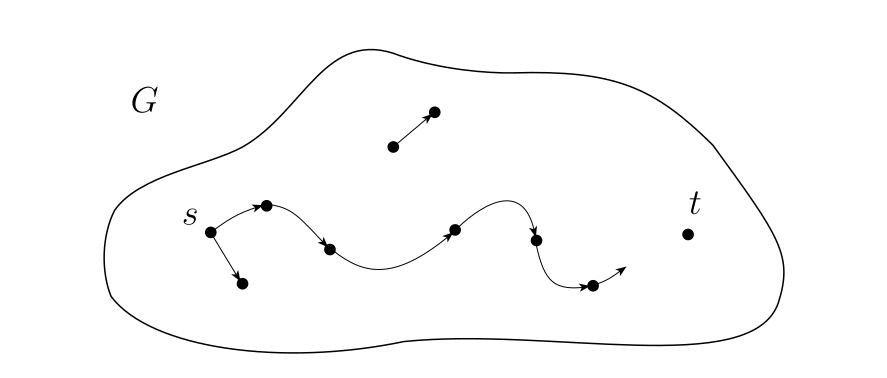
\includegraphics[scale=0.30]{path}
\]
\begin{description}
\item \textit{algoritmo}: 
input $<G,s,t>$
output $si$ se $<G,s,t> \in PATH$, $no$ altrimenti
\begin{enumerate}
\item $M = \{ s \}$
\item cicla fin quando non aggiungo più vertici:
\item \ \ \ \ $M \cup \{ V \ | \ (x, V) \in E, \ x \in M \}$
\item se $t \in M$, rispondo $si$, $no$ altrimenti
\end{enumerate}
\end{description}

\begin{description}
\item \textit{complessità}:
Analizziamo l'algoritmo e mostriamo che ha complessità polinomiale. Il punto 1 e 4 sono eseguiti una sola volta. Il passo 3 è eseguito al più $|V|$ volte. Il numero di esecuzioni delle fasi è quindi al più $1 + 1 + |V|$, quindi polinomiali nella grandezza di $G$. I passi 1 e 4 sono facilmente implementabili in tempo polinomiale. Il passo 3 involve una scansione dell'input e un test per vedere se un vertice è già stato marcato, il che è facilmente implementabile in tempo polinomiale. Quindi $PATH \in P$.
\end{description}

\subparagraph{$E_{DFA}$ è in P} 
\begin{gather*}
E_{DFA} = \{ <A> | A \in DFA \ e \ L(A)=\emptyset \}
\end{gather*}
Per $A \in DFA$ si ha $L(A)=\emptyset$ quando non vi è un cammino dal suo stato di inizio $q_0$ ad un suo stato di accettazione $q_F$. Potendo determinare in tempo polinomiale l'insieme $PATH$ dei nodi per i quali esiste un cammino in $G$, ne concludiamo che potremo calcolare l'insieme $\overline{E_{DFA}}$ in tempo polinomiale, riducendolo al problema $PATH$.
\[
	\overline{E_{DFA}} \leq_{m} PATH
\]

\subsection{Determinare il rifiuto di una NTM}
Data una $T \in  NTM$ che si ferma sempre, definisco una strategia che verifica il rifiuto da parte di $T$ di un dato input $x$. 
Come nell'algoritmo studiato per dimostrare l'equivalenza tra $TM$ e $NTM$, simuliamo la macchina non deterministica $T$, che per ipotesi diciamo avere come grado di non determinismo 2 (e quindi un albero delle configurazioni binario), con una deterministica $T' \in TM$ utilizzando i tre nastri: input, lavoro, guida. Aggiungo questa volta un ulteriore nastro, detto di conteggio. Questo nastro terrà il conto del numero di foglie nell'albero delle configurazioni di $T$ che hanno una configurazione di rifiuto o per cui la configurazione è bloccata. Al termine della simulazione di $T$, se il valore numerico nel nastro di conteggio è uguale a $2^h$, con $h$ altezza dell'albero, allora tutte le foglie sono o di rifiuto o bloccate. Di conseguenza possiamo dire che $T$ non accetta $x$.
\newpage
%!TEX root=../../root.tex

\section{Lezione 18}

\subsection{Complessità di una TM che simula una NTM}

Precedentemente si è indagata l'equivalenza tra macchine di Turing $TM$ e macchine di Turing non deterministiche $NTM$. In particolare sappiamo che 
\[
	T \in NTM \implies \exists \ T' \in TM \text{ tale che } L(T) = L(T')
\]

Cosa possiamo dire dal punto di vista della complessità? Ovvero data $T \in NTM$ e $t_T(n)$ e una $T' \in TM$ equivalente, cosa possiamo dire di $t_{T'}(n)$?

Senza perdere di generalità, assumiamo che $T$ abbia un massimo grado di non determinismo pari a 2, in quanto il ragionamento vale per qualsiasi $k$. Con questa assunzione, l'albero delle configurazioni della $NTM$ è binario. Per definizione di $t_T(n)$, essa è il massimo numero di mosse che la macchina $T$ compie su input di dimensione $n$; di conseguenza per una $NTM$ essa coincide con l'altezza dell'albero, in quanto ogni cammino radice foglia è costituito da al massimo $t_T(n)$ mosse che una "copia" della macchina compie sull'input.

L'albero ha quindi al massimo $2^{t_T(n)}$  foglie, ovvero la $TM$ che simula ha $2^{t_T(n)}$ cammini radice foglia da simulare. Ognuna di queste simulazioni richiede al più $t_T(n)$ mosse. Da queste considerazioni discende che
\[
	t_{T'}(n) = t_{T}(n) \cdot 2^{t_T(n)} = 2^{log(t_T(n))} \cdot 2^{t_T(n)} = 2^{t_T(n) + log(t_T(n))} = 2^{O(t_T(n))}
\]
ovvero una macchina di Turing impiega tempo esponenziale per simulare il non determinismo.

\subsection{La classe NP}

Definiamo $NTIME(n^k)$ l'insieme dei linguaggi per cui esiste una $NTM$ che ne accetta le parole di dimensione $n$ in un numero di passi $O(n^k)$:

\[
	NTIME(n^k) = \{ L \ | \ \exists \ T \in NTM \text{ tale che } L(T) = L \text{ e } t_T(n) = O(n^k) \}
\]

Sulla base di questa definizione introduciamo la classe dei linguaggi (o equivalentemente dei \emph{problemi}) $NP$:
\[
	NP = \bigcup_{k \geq 0} \{ NTIME(n^k) \}
\]

Essa \emph{non} è composta dai problemi non risolvibili polinomialmente, in quanto quella descrizione individua la classe $\overline{P}$. 
\\
Invece di $NP$ fanno parte problemi che si è in grado di risolvere in tempo polinomiale tramite \emph{non determinismo}. Della maggior parte di essi non si ha la certezza che non sia possibile costruire una macchina di Turing, ovvero un algoritmo, che deterministicamente li risolva in tempo polinomiale. Semplicemente un tale algoritmo non è ancora stato trovato.

\subsection{Problemi NP}

\subsubsection{Problema del Cammino hamiltoniano}

\[
	HAMPATH = \{ <G, s, t> \ | \ G \text{ è un grafo diretto con un c.h. da } s \text{ a } t\}
\]

Indichiamo con \emph{c.h.} per brevità un \emph{cammino hamiltoniano}, ovvero una sequenza di nodi $v_1,...,v_n$, dove $n = |V_G|$, con le seguenti proprietà:
\begin{itemize}
	\item $v_1 = s$ e $v_n = t$
	\item $(v_i, v_{i+1}) \in E_G$ per $i = 1, ..., n-1$
\end{itemize}

Per mostrare che $HAMPATH \in NP$, esibiamo una $NTM$ che lo decide in tempo polinomiale.
\\

$T_{HP}$
\begin{description}
	\item[input] $<G, s, t>$

	\item[output] SÌ se $<G,s,t> \in HAMPATH$, NO altrimenti

	\item[descrizione]
	\begin{enumerate}[label*=\arabic*.]
		\item Genera \emph{non deterministicamente} una permutazione $v_1, ..., v_n$ dei nodi di $G$

		\item Verifica che la permutazione generata sia effettivamente un c.h. nel seguente modo:
		\begin{enumerate}[label*=\arabic*.]
			\item Verifica che $v_1$ sia uguale a $s$ e che $v_n$ sia uguale a $t$
			\item Per ogni $v_i, v_{i+1}$ nella permutazione, verifica che vi sia l'arco $(v_i, v_{i+1}) \in E_G$
		\end{enumerate}
	\end{enumerate}
\end{description}

\paragraph{Complessità} Prima di tutto, vediamo come costruire una $NTM$ che genera permutazioni su $\{1, ..., n\}$. Modificando leggermente la macchina che descriveremo, si potranno generare permutazioni anche sui vertici $\{v_1, ..., v_n\}$ di un grafo.
\begin{figure}[H]
	\centering
	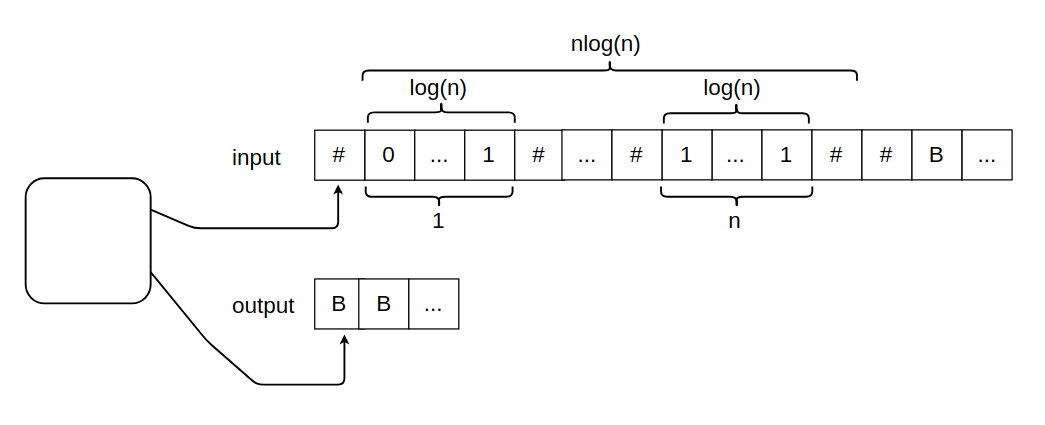
\includegraphics[width=\textwidth]{automa-permutazione}
\end{figure}

Assumiamo che la macchina abbia a disposizione due nastri, uno da cui legge e uno su cui scrive la permutazione; come sappiamo, questa assunzione non è vincolante, ma solo comoda per una descrizione ad alto livello. Assumiamo inoltre che i numeri siano memorizzati sul nastro come si vede in figura. Ogni numero occupa $log(n)$ celle in quanto codificato in binario, ed è separato dal successivo da un separatore $\#$. L'insieme è terminato da un doppio separatore $\#\#$.

\subparagraph{Fase di generazione}

La generazione \emph{non deterministica} della permutazione procede come segue:
\begin{enumerate}[label*=\arabic*.]
	\item se la testina del primo nastro si trova su un separatore (non di fine input) decide se copiare il numero che segue sul secondo nastro o meno:
	\begin{enumerate}[label*=\arabic*.]
		\item se decide di copiarlo:
		\begin{enumerate}[label*=\arabic*.]
			\item marca il primo separatore per ricordarsi che ha copiato il numero 
			\item avanza entrambe le testine scrivendo sul secondo nastro tutto ciò che legge sul primo
			\item quando incontra il separatore successivo, si ferma
		\end{enumerate}
		\item se decide di non copiarlo:
		\begin{enumerate}[label*=\arabic*.]
			\item avanza la testina sul primo nastro fino al separatore successivo, senza fare nulla
		\end{enumerate}
	\end{enumerate}
	\item se l'input è finito (doppio separatore), riporta la testina del primo nastro all'inizio
	\item torna al punto 1, ma se incontra un separatore marcato, avanza al separatore successivo senza toccare il secondo nastro
\end{enumerate}

Vediamo qual è la complessità di questa $NTM$. Assumendo che in ogni scansione decida di copiare almeno un numero (facilmente implementabile), questa effettua al massimo $n$ scansioni del nastro. Come evidenziato in figura, l'input è codificato su $nlog(n)$ celle, per cui ogni "copia" della macchina effettua $n^2 log(n)$ mosse nel generare una permutazione. La macchina quindi non deterministicamente le genera tutte in tempo polinomiale.

Sostituendo le codifiche di $\{1, ..., n\}$ con le codifiche di $\{ v_1, ..., v_n\}$ si ottiene un automa che calcola le permutazioni dei nodi necessarie per $T_{HP}$.

\subparagraph{Fase di verifica}

Le due verifiche possono essere effettuate in tempo polinomiale anche deterministicamente:
\begin{enumerate}[label*=\arabic*.]
	\item \begin{enumerate}[label*=\arabic*.]
		\item copia la codifica di $s$ sul secondo nastro
		\item porta la testina del primo nastro all'inizio di $v_1$, la testina del secondo nastro all'inizio di $s$
		\item avanza contemporaneamente le due testine, verificando l'uguaglianza cella per cella
		\item ripeti per $t$ e $v_n$
	\end{enumerate}
	Complessità logaritmica in $n$, ovvero polinomiale.

	\item Assumendo che gli archi siano codificati sul nastro come una sequenza di coppie di vertici $(u, w)$, si procede così:
	\begin{enumerate}[label*=\arabic*.]
		\item ripeti per ogni $v_i, v_{i+1}$ nella permutazione:
		\begin{enumerate}[label*=\arabic*.]
			\item ripeti per ogni arco $(u, w) \in E$:
			\begin{enumerate}[label*=\arabic*.]
				\item copia la codifica di $(v_i, v_{i+1}) \in permutazione$ all'inizio del secondo nastro, come se fosse un arco
				\item porta la prima testina all'inizio della codifica di $(u, w)$
				\item porta la seconda testina all'inizio della codifica di $(v_1, v_2)$
				\item confronta cella per cella le codifiche di $(u, w)$ e $(v_i, v_{i+1})$ finché non arrivi alla fine della codifica
				\item riporta la testina sul secondo nastro all'inizio del nastro
			\end{enumerate}
		\end{enumerate}
	\end{enumerate}
	Al più gli archi possono essere $n^2$, perciò la porzione da scandire è lunga $n^2 log n$. Si effettuano $n$ scansioni, per cui la complessità è $n \cdot n^2log(n) = n^3 log(n)$, ovvero polinomiale.
\end{enumerate}
Notiamo quindi che l'unica \emph{fase non deterministica} è la \emph{fase di generazione}, mentre la \emph{fase di verifica} può essere effettuata deterministicamente in tempo polinomiale.

\subsubsection{Problema del Clique}
Dato un grafo qualsiasi $G$, un $k$-clique è un sottoinsieme $C$ dei suoi vertici tale che ogni vertice è connesso con ogni altro
\[
	v_i, v_j \in C \implies \{v_i, v_j\} \in E
\]
Il problema del Clique consiste, dato un grafo, nel trovare il clique di cardinalità massima. Esso non è dunque un problema di \emph{decisione}, bensì un problema di \emph{ottimizzazione}. Consideriamo tuttavia il problema di decisione associato, parametrizzando per la cardinalità $k$ del clique cercato:

\[
	CLIQUE(k) = \{ <G, k> \ | \ G \text{ è un grafo con un } k\text{-clique} \}
\]
Il problema di ottimizzazione può quindi essere risolto sfruttando il problema di decisione, nel seguente modo:
\IncMargin{1em}
\begin{algorithm}
\SetKwInOut{Input}{input}\SetKwInOut{Output}{output}

\Input{Un grafo $G$}
\Output{La cardinalità della clique di cardinalità massima}
\BlankLine
\For{i = n $\to$ 1}{
	\If{$<G, i> \in CLIQUE(k)$}{
		\Return i\;
	}
}
\end{algorithm}\DecMargin{1em}

\newpage

Come prima, esibiamo una $NTM$ che decide $CLIQUE(k)$ in tempo \\
polinomiale:
\\

$T_{C}$
\begin{description}
	\item[input] $<G, k>$
	\item[output] SÌ se $<G, k> \in CLIQUE(k)$, NO altrimenti
	\item[descrizione]
	\begin{enumerate}[label*=\arabic*.]
		\item genera non deterministicamente un sottoinsieme $S$ \emph{qualunque} dei nodi di $G$

		\item verifica che $S$ sia un $k$-clique, ovvero:
		\begin{enumerate}[label*=\arabic*.]
			\item $|S| = k$
			\item $u, v \in S \implies \{u, v\} \in E$
		\end{enumerate}
	\end{enumerate}
\end{description}

\paragraph{Complessità}

Un automa che genera sottoinsiemi è molto simile a quello che genera permutazioni, descritto precedentemente: l'automa per ogni nodo sul primo nastro decide non deterministicamente se copiarlo o meno sul secondo nastro, in un'unica scansione. Così una "copia" dell'automa, andando con la testina su $v_1$, deciderà di copiarlo, decidendo invece di non copiare nessun altro nodo; un'altra invece deciderà di copiare ogni nodo, e così via.
\\

Ogni copia della macchina effettua un'unica scansione del nastro, che per quanto detto prima richiede $nlog(n)$ mosse. Ne consegue che anche in questo la complessità della \emph{fase non deterministica} è polinomiale. La \emph{fase di verifica}, similmente al problema del cammino hamiltoniano, può essere eseguita \emph{deterministicamente} in tempo polinomiale. 

\subsection{Verificatore polinomiale}

Nei due esempi precedenti si è visto come la \emph{fase di verifica} potesse essere eseguita \emph{deterministicamente} e in tempo \emph{polinomiale}. È quindi lecito chiedersi se questa sia una proprietà comune a tutti i problemi $NP$. Questo permetterebbe una definizione dei problemi $NP$ che ignora completamente il concetto del non determinismo. 

Introduciamo formalmente il concetto di \emph{verificatore}:
\begin{gather*}
	V \in TM \ verifica \ A \text{ se} \\
	A = \{ w \ | \ (w, c) \in L(V) \text{ per un qualche } certificato \ c \}
\end{gather*}
L'aggiunta di \emph{polinomiale} significa che il verificatore opera in una serie polinomiale di passi, cioè $t_V(n) = O(n^k)$.\\
Un \emph{certificato} è una possibile soluzione di una istanza di un problema, un concetto meglio comprensibile tramite un esempio. 
\\
Forniamo a tale scopo un verificatore per il problema di decisione $CLIQUE(k)$.
\\

$V_{CLIQUE}$:
\begin{description}
	\item[input] $(<G, k>, c)$
	\item[output] SÌ se $c$ è un $k$-clique di $G$, NO altrimenti
	\item[descrizione] semplicemente effettua la verifica esposta in precedenza
\end{description}

Come si vede, è più comodo esibire un verificatore rispetto ad esibire una $NTM$ che decide un problema. Vediamo un altro esempio.

\subsubsection{Problema dei numeri composti}
Istanze sì del problema sono tutti quei numeri \emph{composti}, ovvero non primi, per cui si riesce a trovare un naturale diverso da $1$ e da sè stesso che lo divide.
\[
	COMPOSITES = \{ p \ | \ p \in \mathbb{N} \text{ e } \exists \ q, r \in \mathbb{N} \text{ con } p = q \cdot r \text{ con } q \neq 1, q \neq n\}
\]

Esibiamo sia un $T_{COMP} \in NTM$ che lo decide, sia un verificatore $V_{COMP}$ che lo verifica.
\begin{itemize}
	\item $T_{COMP}$
	\begin{description}
		\item[input] $p \in \mathbb{N}$
		\item[output] SÌ se $p$ è composto, NO altrimenti
		\item[descrizione]
		\begin{enumerate}
			\item genera non deterministicamente tutti i naturali $q$ con $1 < q < p$

			\item verifica se $p \ mod \ q \equiv 0$
		\end{enumerate}
	\end{description}

	\item $V_{COMP}$
	\begin{description}
		\item[input] $(p, c)$ con $p, c \in \mathbb{N} $
		\item[output] SÌ se $c$ divide $p$, NO altrimenti
		\item[descrizione]
		\begin{enumerate}
			\item verifica se $c \neq 1$ e se $c < p$
			\item verifica se $p \ mod \ c \equiv 0$
		\end{enumerate}
		
	\end{description}
\end{itemize}
Anche questo problema sta in $NP$, e anche in questo caso siamo riusciti ad esibire un verificatore polinomiale. Come accennato precedentemente, questa è effettivamente una proprietà comune a tutti i problemi in $NP$.

\subsection{Dimostrazione NP = VP}

Definiamo $VP = \{ L \ | \ \exists \text{ verificatore polinomiale } V \text{ che verifica } L \}$. La dimostrazione, come di consueto, procede per \emph{doppia inclusione}.


\paragraph{NP $\subseteq$ VP}

Vogliamo mostrare che $L \in NP \implies \exists V \in VP \text{ che lo verifica}$.
\\
\\
Se $L \in NP$ allora per definizione $\exists \ T \in NTM$ con $t_T(n) = O(n^k)$, per qualche $k$, tale che $L(T) = L$. Costruiamo un verificatore per $L$.

Supponiamo che l'albero di computazione di $T$ abbia massimo grado di non determinismo uguale a 2. Inoltre, come visto in precedenza, esso sarà alto $t_T(n)$.
Costruiamo allora un certificato $c \in \{0,1\}^{\star}$, con $|c| = t_T(n)$. Un certificato del genere è in grado di identificare univocamente ogni cammino radice foglia, ovvero un percorso di computazione. Il verificatore $V_L$ è allora così composto:
\begin{description}
	\item[input] $<w, c>$
	\item[descrizione]
	\begin{enumerate}
		\item esegui $T$ su $w$ seguendo il percorso di computazione identificato da $c$
		\item se $T$ accetta, allora accetta
		\item se $T$ rifiuta, allora rifiuta
	\end{enumerate}
\end{description}

La costruzione del verificatore è corretta perché possiamo esprimere $L(T)$ secondo la definizione di verificatore:
\[
	L(T) = \{w \ |\ <w, c > \in L(V_L) \text{ per qualche certificato } c \}
\]
Infatti per ogni parola $w$ accettata da $T$ esiste almeno un cammino di accettazione per $w$, dunque per costruzione esiste un
certificato $c$ per cui $V_L$ accetta. 
\\
Se invece $w$ è rifiutata da $T$, allora nessun cammino è di accettazione, quindi nessun certificato identifica un cammino di accettazione, quindi $V_L$ rifiuta $w$ su qualsiasi certificato.
\\
Inoltre la complessità è polinomiale perché la sequenza $c$ è di lunghezza polinomiale, e quindi anche il numero di passi di $T$ che $V_L$ simula è polinomiale.

\paragraph{VP $\subseteq$ NP} 

Vogliamo mostrare che $L \in VP \implies \exists T \in NP \text{ che lo decide}$.
\\
\\
Se $L \in VP$ allora per definizione $\exists \ V$ tale che $ L = \{ w \ | \ <w, c> \in L(V) \}$ con $t_V(n) = O(n^k)$. Costruiamo una $T_L \in NTM$ che decide $L$.
\\

$T_L$
\begin{description}
	\item[input] $w$ 
	\item[output] SÌ se $w \in L$, NO altrimenti
	\item[descrizione]
	\begin{enumerate}[label*=\arabic*.]
		\item genera non deterministicamente tutti i certificati $c$ con $|c| \leq t_V(n)$

		\item esegui il verificatore su $<w, c>$
		\begin{enumerate}[label*=\arabic*.]
			\item se $V$ accetta, allora accetta
			\item se $V$ rifiuta, allora rifiuta
		\end{enumerate}
	\end{enumerate}
\end{description}

La costruzione è corretta in quanto se $w \in L$ allora esiste almeno un certificato $c$ per cui $V$ accetta $<w, c>$. Poiché $T_L$ genera non deterministicamente \emph{tutti} i certificati, necessariamente genera anche $c$, e un suo cammino di computazione esegue $V$ su $<w, c>$, il quale per quanto detto prima accetta, e quindi esiste un cammino di accettazione di $T_L$ per $w$.
\\
Se invece $w \notin L$ allora non esiste un certificato $c$ per cui $V$ accetta $<w, c>$. Quindi per \emph{nessun} certificato generato da $T_L$ si avrà l'accettazione di $V$ su $<w, c>$. Ne segue che non esiste un cammino di accettazione di $T_L$ per $w$, ovvero $T_L$ rifiuta $w$.

\newpage
%!TEX root=../../root.tex

\newpage

\section{Lezione 19}

\subsection{\texorpdfstring{$\overline{HAMPATH}$}{HAMPATH negato} \texorpdfstring{$\notin$}{non appartiene a} NP}

\begin{figure}[H]
    \centering
    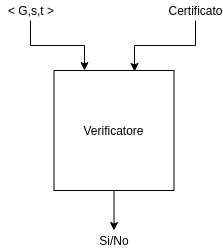
\includegraphics[scale=0.60]{notHam}
\end{figure}

\begin{gather*}
	\overline{HAMPATH} = \{ <G, s, t> \ | \ G \text{ è un grafo diretto senza cammini hamiltoniani} \\
	\text{da } s \text{ a } t \}
\end{gather*}
Il problema $\overline{HAMPATH}$ non è in $NP$ poiché non ammette un verificatore polinomiale, in quanto tale verificatore dovrebbe controllare che \textit{nessuna} permutazione di nodi sia un cammino hamiltoniano. Quindi il certificato da dare al verificatore dovrebbe necessariamente contenere tutte le possibili permutazioni dei vertici ed avere quindi tale dimensione (esponenziale), mentre nel caso di $HAMPATH$ era sufficiente fornire una possibile permutazione dei vertici come certificato.

\subsection{Relazione fra P e NP}

Uno dei maggiori problemi irrisolti dell'informatica teorica è quello di stabilire quale relazione lega $P$ ed $NP$, vi sono due possibilità:

\begin{figure}[H]
    \centering
    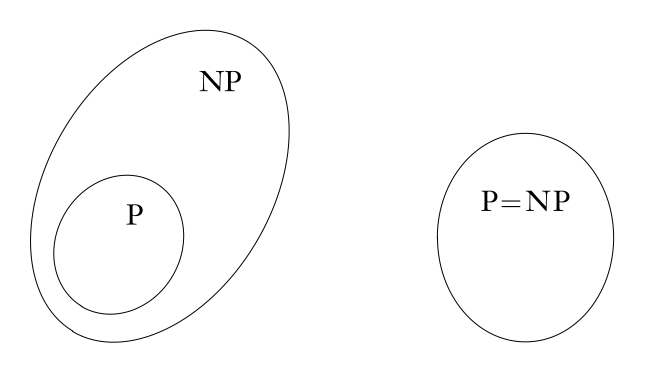
\includegraphics[scale=0.40]{PNP}
\end{figure}

Definiamo $ EXPTIME = \displaystyle \bigcup_{k \geq 0}{TIME(2^{O(n^k)})} $, 
sappiamo che $ NP \subseteq EXPTIME$ poiché si è visto che una $TM$ simula una $NTM$ con complessità di tempo $2^{O(t(n))}$, ma non sappiamo se esista una classe di complessità deterministica più piccola di $EXPTIME$ che contenga $NP$. 

Per dimostrare $P=NP$ si è cercato senza successo un metodo alternativo polinomiale per convertire una NTM in una TM deterministica, mentre per dimostrare $P\subsetneq NP$ si è cercato un problema in $NP$ con un limite inferiore non in $P$.


\subsection{Riduzione Polinomiale}

Un linguaggio $A$ si \textit{riduce polinomialmente} a un linguaggio $B$, ovvero in simboli $A \leq_p B$ se:
\[
   \exists \ f: \Sigma^{\star} \rightarrow \Sigma^{\star} \ \text{tale che}
\]
\begin{enumerate}
    \item \textit{f} è calcolabile in tempo polinomiale 
    \item $ x \in A \iff f(x) \in B $
\end{enumerate}

\subsection{I linguaggi CNFSAT e 3SAT}

\[
    CNFSAT = \{ \ \varphi \ | \ \varphi \in CNF \ \land \varphi \ \text{è soddisfacibile} \}
\]
Con $CNF$ si intende la Forma Normale Congiuntiva di una formula booleana, ovvero formata solo da \textit{clausole} in \textit{and}. Una clausola è un insieme di letterali in \textit{or}.

Si verifica facilmente l'appartenenza di CNFSAT ad NP esibendo un verificatore $V$:
\begin{description}
    \item \textit{input}: $<\varphi, s>$, con $\varphi \in CNF$ e $s \in \{0, 1\}^{\star}$ che rappresenta una assegnazione di verità ad ogni letterale (variabile o sua negazione) in $\varphi$

    \item \textit{descrizione}: verifica che ogni clausola valutata su tale assegnamento di letterali sia vera
\end{description}

Introduciamo ora il linguaggio $3SAT$, che in quanto sottoinsieme di $CNFSAT$, è in $NP$
\[
    3SAT = \{ \ \varphi \ | \ \varphi \in CNF  \text{ soddisfacibile } \land \text{ogni clausola è di 3 letterali} \}
\]

\paragraph{La riduzione}

\[
	\varphi = C_1 \land \dots \land C_k \text{ con } C_i \text{ clausola}
\]
Trasformiamo ogni clausola in una 3-clausola equivalente: sia 
\[
	C = X_1 \lor \dots \lor X_m
\] 
una generica clausola. La trasformazione è così descritta:

\begin{enumerate}
    \item $m=1$ \quad $C = X_1 \Rightarrow \varphi_C = X_1 \lor X_1 \lor X_1$
    \item $m=2$ \quad $C = X_1 \lor X_2 \Rightarrow \varphi_C = X_1 \lor X_2 \lor X_1$
    \item $m=3$ \quad C è già una 3-clausola
    \item $m\geq 4$
\begin{gather*}
	\varphi_C = \left( X_1 \lor X_2 \lor Z_1 \right) \land
		\left( \overline{Z_1} \lor X_3 \lor Z_2 \right) \land \dots \land
        \left( \overline{Z_{i-2}} \lor X_i \lor Z_{i-1} \right) \\
        \land \dots \land \left( \overline{Z_{m-3}} \lor X_{m-1} \lor X_{m} \right)
\end{gather*}
\end{enumerate}

Nei primi tre casi è ovvio che $C \text{ soddisfacibile} \Rightarrow \varphi_C$ soddisfacibile; nel quarto caso un po' meno, e lo mostreremo esplicitamente.

\subparagraph{C è soddisfatta $\Rightarrow \varphi_C$ è soddisfatta}
$$C \ \text{soddisfatta} \Rightarrow \ \exists \ i \ | \ X_i=1, \ 1\leq i \leq m$$
\begin{align}
 & i = 1,2  & & \Rightarrow Z_j = 0 & \forall \ 1\leq j \leq m-3  \\
 & i = m-1,m & & \Rightarrow Z_j = 1  & \forall \ 1\leq j \leq m-3 \\
 & 2 < i < m-1 &  & \Rightarrow Z_j = 1  & \forall  \ 1 \leq j \leq i-2 \\  
 & & & \text{e} \ \ \ Z_j = 0 &  \forall \ \ i-1\leq j \leq m-3 \nonumber
\end{align}
Se $X_1$ o $X_2$ sono vere, allora la prima clausola è vera: costruire una $\varphi_C$ con tutte le $Z_j = 0$ fa sì che tutte le clausole intermedie siano vere, in quanto contengono la negazione di una qualche $Z_k$, e così anche l'ultima che contiene $\overline{Z_{m-3}}$.

Se $X_{m-1}$ o $X_m$ sono vere, allora l'ultima clausola è vera: costruire una $\varphi_C$ con tutte le $Z_j = 1$ fa sì che tutte le clausole intermedie siano vere, similmente a prima, e così anche la prima che contiene $Z_1$.

Se infine è l'assegnamento di una qualche $X_i$ intermedia a rendere soddisfatta $C$, allora l'$i$-esima clausola è vera, e bisogna far sì che lo siano anche tutte le altre. Costruendo $\varphi_C$ con $Z_j = 1$ fino a $j = i-2$, le clausole precedenti sono sicuramente vere, in quanto ogni clausola (inclusa la prima) contiene un letterale vero; se $Z_j = 0$ da $j=i-1$ in poi, le clausole successive sono sicuramente vere, in quanto ogni clausola (inclusa l'ultima) contiene un letterale che è la negazione di una variabile falsa.

\subparagraph{$\varphi_C$ soddisfatta $\Rightarrow C$ soddisfatta}
\quad
Supponiamo per assurdo che C non sia soddisfatta dall'assegnamento che rende vera $\varphi_C$, cioè $X_i = 0 \quad \forall \ 1 \leq i \leq m$.

Se $X_i = 0 $ allora a rendere vere le clausole di $\varphi_C$ dovrebbero essere le $Z_i$: se fosse $Z_i = 1$ per ogni $i$, allora l'ultima clausola sarebbe falsa; se fosse $Z_i = 0$ per ogni $i$, allora la prima clausola sarebbe falsa; in generale qualunque fosse l'assegnamento delle $Z_i$, ci sarebbe almeno una clausola di $\varphi_C$ falsa, e quindi $\varphi_C$ non sarebbe soddisfatta in contraddizione con l'ipotesi.

\subsection{Teorema di Cook-Levin}

\paragraph{NP-completezza}
Un linguaggio $A$ è detto $NP$-completo se soddisfa due condizioni:
\begin{enumerate}
    \item $\forall B \in NP$, $B \leq_{p} A$ (A è NP hard)
    \item $A \in NP$
\end{enumerate}
Cook e Levin introdussero il concetto di \textit{NP-completezza}, ovvero la proprietà di un linguaggio per cui qualsiasi altro linguaggio in $NP$ si può ridurre polinomialmente ad esso. Essi dimostrarono che $SAT$ (e in particolare $CNFSAT$) è $NP$-completo, con una dimostrazione che non vediamo in quanto lunga, poiché deve prendere in esame un linguaggio $L$ generico e mostrare che $L \leq_p SAT$.

\paragraph{Transitività della riduzione} $A \leq_p B \leq_p C \implies A \leq_p C$

\subparagraph{Dimostrazione}
Sia $f$ la funzione di riduzione per $A \leq_p B$ e $T_f$ una $TM$ che la calcola in tempo polinomiale $O(n^k)$. 

Sia inoltre $g$ la funzione di riduzione per $B \leq_p C$ e $T_g$ una $TM$ che la calcola in tempo polinomiale $O(n^{k'})$.

Allora è possibile comporre $T_f$ e $T_g$ ottenendo una $TM$ che, dato un $x \in A$, calcola $g(f(x)) \in C$ in un tempo polinomiale $O((n^k)^{k'}) = O(n^{k \cdot k'}) = O(n^{k''})$.

Grazie a questa proprietà, per mostrare che un linguaggio è $NP$-hard basta mostrare che sia possibile ridurre polinomialmente $CNFSAT$ ad esso. Infatti se $CNFSAT \leq_p A$, allora significa che per qualunque $B \in NP$ vale $B \leq_p CNFSAT \leq_p A$, ovvero $B \leq_p A$ ovvero $A$ è $NP$-hard. Se si sa che $A \in NP$, allora $A$ è anche $NP$-completo. Ad esempio, abbiamo mostrato che $CNFSAT \leq_p 3SAT$, e poiché $3SAT \in NP$, possiamo affermare che $3SAT$ è $NP$-completo.

\paragraph{Lemma}
Se un linguaggio è riducibile polinomialmente a un linguaggio in $P$, allora anche esso è in $P$.
\[
        B \in P \land A \leq_{p} B \implies A \in P
\]

\paragraph{Enunciato} 
\[
B \text{ è } NP\text{-completo } \land B \in P \implies P = NP
\]
\paragraph{Dimostrazione}

Se $B$ è $NP$-completo allora ogni altro linguaggio $A \in NP$ si riduce polinomialmente ad esso. Ma $B \in P$, allora per il lemma precedente qualsiasi $A$ che si riduce polinomialmente a $B$ è anch'esso in $P$. Dunque tutti i linguaggi in $NP$ stanno anche in $P$, dimostrando che $NP \subseteq P$, ovvero l'inclusione mancante per dimostrare $P = NP$.

\subsection{Esempi di riduzioni polinomiali}
\subsubsection{Clique}
\[
	CLIQUE(k) = \{ <G,s,t> \ \mid \ \text{G ha un clique di k-elementi} \}
\]	
Per affermare che $CLIQUE(k)$ sia $NP$-completo bisogna mostrare che:
\begin{enumerate}
    \item CLIQUE(k) $\in$ NP (vedi 18.3.2)
    \item 3SAT $\leq_{p}$ CLIQUE 
\end{enumerate}
Dobbiamo quindi esibire una $f$ di riduzione, calcolabile polinomialmente, tale che:
\[
	\varphi \xmapsto{f} <G,k> \text{ tale che } \varphi \text{ è soddisfacibile } \iff G_{\varphi} \text{ ha un clique di k-elementi}
\]

La $f$ costruisce il grafo $G$ nel seguente modo:
\begin{itemize}
	\item ogni nodo nel grafo corrisponde a un letterale presente nelle clausole di $\varphi$

	\item i nodi corrispondenti a letterali nella stessa clausola non sono connessi

	\item i nodi corrispondenti a letterali contraddittori non sono connessi

	\item tutti gli altri nodi sono connessi
\end{itemize}

\paragraph{Esempio}

\[
    \varphi = (X_1 \lor X_1 \lor X_2) \land (\overline{X_1} \lor \overline{X_2} \lor \overline{X_2}) \land (\overline{X_1} \lor X_2 \lor X_2)
\]
e il grafo che costruiamo è il seguente
\begin{figure}[H]
  \centering
  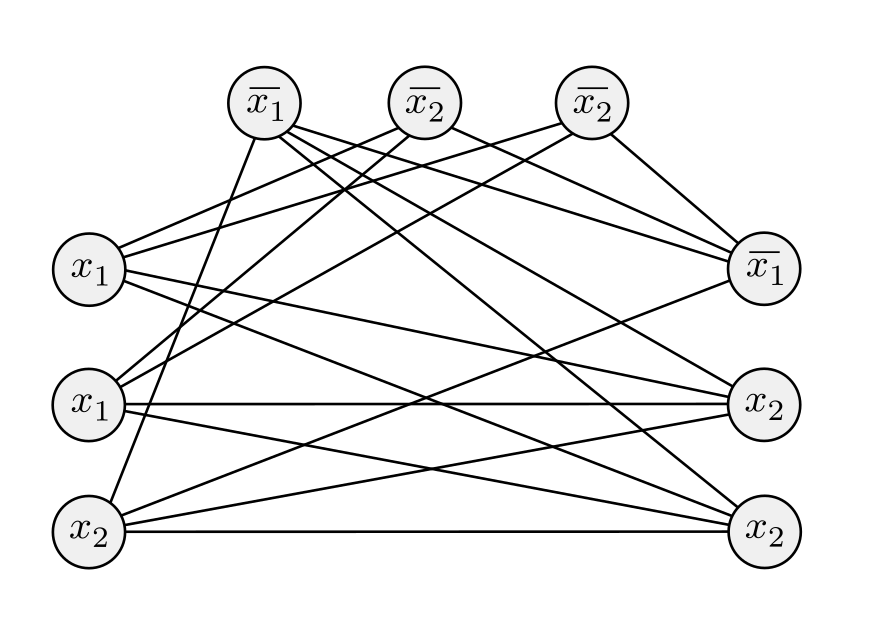
\includegraphics[scale=0.35]{GrafoClique}
\end{figure}

\paragraph{$\varphi$ soddisfacibile $\Rightarrow G_{\varphi}$ ha un $k$-clique}

Se $\varphi$ è soddisfacibile, e  $\varphi = C_1 \ \land \ C_2 \ \land$ \\
$\land \dots \land \ C_n$, allora essa ha un qualche assegnamento di verità che la rende soddisfatta. Consideriamo tale assegnamento: in ogni $C_i$ vi è almeno un letterale vero, che indichiamo con $X_i$. Costruiamo $G_{\varphi}$ con la regola di cui sopra e consideriamo i nodi etichettati con i vari $X_i$: essi sono $k$, tanti quante le clausole, e inoltre sicuramente sono connessi tra loro poiché, considerati a coppie
\begin{enumerate}
	\item non appartengono alla stessa clausola $C_i$

	\item non sono contraddittori, poiché se lo fossero allora o uno dei due non sarebbe vero (contraddizione), oppure $\varphi$ sarebbe contraddittoria (contraddizione)
\end{enumerate}
Quindi il sottografo formato dai nodi etichettati con i vari $X_i$ è una $k$-clique.

\paragraph{$G_{\varphi}$ ha un $k$-clique $\Rightarrow \varphi$ è soddisfacibile}
Se $G_{\varphi}$ ha un $k$-clique, nessun nodo nel clique corrisponde a letterali appartenenti alla stessa clausola, in quanto per costruzione essi non sono connessi. Di conseguenza ogni clausola contiene esattamente 1 letterale corrispondente a un nodo nel clique, perciò basta trovare un assegnamento di verità che rende vero ognuno di questi letterali per rendere soddisfatta $\varphi$. 

Tale assegnamento esiste sicuramente, in quanto i letterali del clique non sono contraddittori, altrimenti per costruzione non sarebbero connessi, e quindi non potrebbero far parte del $k$-clique (contraddizione).

Quindi $\varphi$ è soddisfacibile.

\subsubsection{IndSet}
\[
	INDSET = \{ <G,k> \ \mid G\text{ ha un independet-set di k-elementi}\}
\]
Con \textit{independet-set} si indica un sottoinsieme $S$ di nodi di $G$ per cui $v, w \in S \implies \{v, w\} \notin E_G$. 

Mostriamo che $INDSET$ è $NP$-completo:
\begin{enumerate}
    \item INDSET $\in$ NP (si verifica facilmente)
    \item 3SAT $\leq_{p}$ INDSET
\end{enumerate}

Come al solito, dobbiamo esibire una $f$ di riduzione per cui:
\begin{gather*}
	\varphi \xmapsto{f} <G_{\varphi}, k> \text{ tale che} \\
	\varphi \text{ ha k clausole ed è soddisfatta } \iff G \text{ ha un independent-set di dimensione k}
\end{gather*}

La $f$ costruisce $G$ nel seguente modo:
\begin{itemize}
	\item ogni nodo nel grafo corrisponde a un letterale presente nelle clausole di $\varphi$

	\item i nodi corrispondenti a letterali nella stessa clausola sono connessi

	\item i nodi corrispondenti a letterali contraddittori sono connessi

	\item tutti gli altri nodi non sono connessi
\end{itemize}

\newpage

\paragraph{Esempio}
\begin{equation*}
    \varphi = (X_1 \lor \overline{X_2} \lor X_1) \land (X_2 \lor \overline{X_1} \lor X_3) \land (X_1 \lor X_2 \lor X_3)
\end{equation*}

\begin{figure}[H]
  \centering
  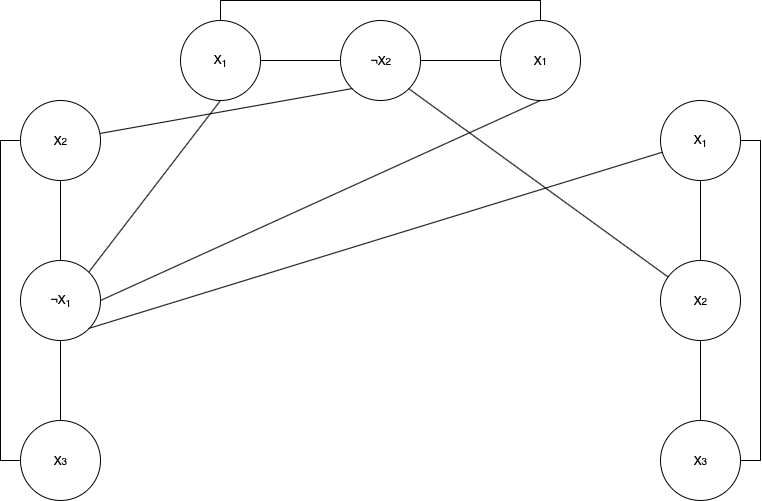
\includegraphics[scale=0.35]{IndSet}
\end{figure}

\paragraph{$\varphi$ soddisfacibile $\Rightarrow G_{\varphi}$ ha un independent-set di dimensione $k$}
Se $\varphi$ è soddisfacibile, e  $\varphi = C_1 \ \land \ C_2 \ \land \dots \land \ C_n$, allora essa ha un qualche assegnamento di verità che la rende soddisfatta. Consideriamo tale assegnamento: in ogni $C_i$ vi è almeno un letterale vero, che indichiamo con $X_i$. Costruiamo $G_{\varphi}$ con la regola di cui sopra e consideriamo i nodi etichettati con i vari $X_i$: essi sono $k$, tanti quante le clausole, e inoltre sicuramente \textit{non} sono connessi tra loro poiché, considerati a coppie
\begin{enumerate}
	\item non appartengono alla stessa clausola $C_i$

	\item non sono contraddittori, poiché se lo fossero allora o uno dei due non sarebbe vero (contraddizione), oppure $\varphi$ sarebbe contraddittoria (contraddizione)
\end{enumerate}
Quindi il sottografo formato dai nodi etichettati con i vari $X_i$ è un independent-set di dimensione $k$.

\paragraph{$G_{\varphi}$ ha un independent-set di dimensione $k$ $\Rightarrow \varphi$ è soddisfacibile}
Se $G_{\varphi}$ ha un independent-set di dimensione $k$, che chiamiamo $S$, allora nessun nodo in $S$ corrisponde a letterali appartenenti alla stessa clausola, in quanto per costruzione essi sono connessi. Di conseguenza ogni clausola contiene esattamente 1 letterale corrispondente a un nodo in $S$, perciò basta trovare un assegnamento di verità che rende vero ognuno di questi letterali per rendere soddisfatta $\varphi$. 

Tale assegnamento esiste sicuramente, in quanto i letterali in $S$ non sono contraddittori, altrimenti per costruzione sarebbero connessi, e quindi non potrebbero far parte di $S$ (contraddizione).

Quindi $\varphi$ è soddisfacibile.
\newpage
%!TEX root=../../root.tex
\section{Lezione 20}

\subsection{Complessità di Spazio}

Sia $M$ una macchina di Turing deterministica che si arresta su tutti gli input. La \emph{complessità di spazio} di $M$ è la funzione 
\begin{gather*}
	f:\mathbb{N} \to \mathbb{N}\\
	f(n) = max\{ \text{numero di celle del nastro che } M \text{ scandisce su ogni input di lunghezza } n \}
\end{gather*}
Se $M$ è una macchina di Turing non deterministica in cui tutte le diramazioni si arrestano su tutti gli input, definiamo la sua complessità di spazio \emph{f(n)} come il massimo numero di celle del nastro che \emph{M} scandisce su qualsiasi diramazione della sua computazione per ogni input di lunghezza \emph{n}.

\subsection{Teorema di Savitch}
\newtheorem*{thm}{Teorema}
\begin{thm} 
Se $T \in NTM$ ha complessità di spazio $S_{T}(n)\geq n$, allora $\exists$ $T' \in TM$ equivalente avente complessità di spazio $S_{T'}(n)=O(S^{2}_{T}(n))$. \\
\end{thm}
\begin{proof}[Dimostrazione]
Il teorema si dimostra esibendo una $TM$ deterministica che simula la $NTM$ data in input, che ha complessità di spazio $S_{T}(n)$, usando spazio $O(S^{2}_{T}(n))$.

L'approccio utilizzato per simulare una $NTM$ con una $TM$ deterministica che conosciamo richiede tempo e spazio esponenziali, quindi si usa un approccio differente. Si consideri il problema più generale del \emph{reach}, la cui formulazione è la seguente:

Date due configurazioni $c, c'$ della $NTM$, determinare se essa può transitare da  $c \  \text{a} \ c'$ in al più $t$ passi. Vediamo una implementazione ricorsiva di tale algoritmo.
\paragraph{CANYIELD}
\begin{description}
	\item \textit{input}: \emph{(c,c',t)}
	\item \textit{output}: 1 se $c \Rightarrow^{\star} c'$ in al più \emph{t} passi, 0 altrimenti
	\item \textit{descrizione}:
	\begin{enumerate}[label*=\arabic*.]
		\item Se $t = 0$:
		\begin{enumerate}[label*=\arabic*.]
			\item Se $c = c'$, allora ritorna 1 
			\item Altrimenti ritorna 0 
		\end{enumerate}
		\item Se $t=1$:
			\begin{enumerate}[label*=\arabic*.]
				\item Se $c \Rightarrow c'$, allora ritorna 1
				\item Altrimenti ritorna 0
			\end{enumerate}
		\item $\forall \ c'' \ \text{di} \ T$
			\begin{enumerate}[label*=\arabic*.]
				\item Ritorna \emph{CANYIELD($c$,$c''$,$\frac{t}{2}$)} $\land$ \emph{CANYIELD($c''$,$c'$,$\frac{t}{2}$)}
			\end{enumerate}
	\end{enumerate}
\end{description}
Risolvere tale problema con input ($c_i,c_f,S_T(n)$), dove $c_i$, $c_f$ e $S_T(n)$ sono rispettivamente la configurazione iniziale $(q_0x)$, la configurazione finale $(q_aB)$ e il numero massimo di passi che la $NTM$ può effettuare, equivale a stabilire se la macchina $T$ accetti o no l'input $x$. \\
Notare che esistono diverse possibili configurazioni finali ma per evitare di dover chiamare l'algoritmo per ogni configurazione accettante applichiamo una modifica alla $NTM$ in modo che l'unica configurazione di accettazione sia proprio $q_aB$, ossia quella in cui il nastro è vuoto e la la testina è all'inizio del nastro.
\begin{figure}[H]
    \centering
    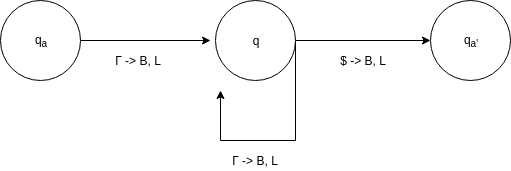
\includegraphics[scale=0.6]{modifica}
\end{figure}

Per capire quanto spazio richiede l'algoritmo analizziamo lo stack delle chiamate ricorsive. Ciascun livello della ricorsione usa spazio \emph{$O(S_{T}(n))$} per memorizzare una configurazione. La profondità della ricorsione è \emph{log t}, dove \emph{t} è il tempo massimo che la NTM può usare su ogni diramazione e che per semplicità assumiamo essere una potenza di 2. Quindi una volta che la ricorsione raggiunge il caso base nello stack delle chiamate ci saranno $O(lg \ t)$ chiamate, ognuna delle quali avrà memorizzato due configurazioni e il valore di t occupando uno spazio di $O(S_T(n)) + O(lg \ t)$.

 Nel nostro caso ci interessa $t=2^{O(S_{T}(n))}$, poiché esso è il tempo che la $TM$ impiega a simulare la $NTM$; quindi $log \ t = O(S_{T}(n))$. Pertanto la simulazione deterministica usa spazio $O(S^2_{T}(n))$.\\
Dobbiamo ora dare la descrizione della macchina deterministica $T'$ equivalente a $T$.

\newpage
$T'$:
\begin{description}
	\item \textit{input: x}  
	\item \textit{descrizione:}
	\begin{enumerate}[label*=\arabic*.]
		\item Esegue \emph{CANYIELD} su ($c_i,c_a,2^{O(S_T(n))}$)
		\begin{enumerate}[label*=\arabic*.]
			\item Se \emph{CANYIELD} ritorna 1, accetta
			\item altrimenti rifiuta
		\end{enumerate}
	\end{enumerate}
\end{description}
L'algoritmo richiede tuttavia in input il parametro \emph{t} che nel nostro caso è $2^{O(S_T(n))}$. Non sapendo $S_T(n)$ dobbiamo sfruttare il fatto che $2^{O(S_T(n))} = 2^{k\cdot S_T(n)}$, $k$ dipende solo da $|\Gamma|$ e $|Q|$ ed è quindi nota, invece per trovare $S_T(n)$  dobbiamo provare tutti i possibili valori $i = 0,1,\dots$ finché non si ottiene l'$S_T(n)$ cercato.

Per far in modo che l'algoritmo si fermi sempre bisogna inoltre controllare ad ogni iterazione che vi sia una configurazione raggiungibile a distanza $i+1$.
\end{proof}

\subsection{PSPACE e NPSPACE}
Per definire le classi $PSPACE$ e $NPSPACE$, ci serviamo di altri due linguaggi ovvero $SPACE$ e $NSPACE$:

$$NSPACE(n^k) = \{ L \mid L \in NTM \land L(T)=L \land S_T(n)=O(n^k) \}$$

$$NPSPACE = \bigcup_{k\geq 0} NSPACE(n^k)$$

$$SPACE = \{ L \mid L \in TM \land L(T)=L \land S_T(N)=O(n^k) \}$$

$$PSPACE = \bigcup_{k\geq 0} SPACE(n^k)$$
\\
Dimostriamo l'uguaglianza tra i due linguaggi appena definiti sfruttando la doppia inclusione, banalmente possiamo vedere che $PSPACE \subseteq NPSPACE$ poiché ogni macchina deterministica è anche non deterministica, e per il \emph{Teorema di Savitch} abbiamo che $NPSPACE \subseteq PSPACE$.
\subsubsection{Relazione PSPACE e NP}
Siccome il tempo utilizzato da una macchina limita la quantità di spazio che la macchina utilizzerà, allora $NP \subseteq NPSPACE$, e data l'uguaglianza tra NPSPACE e PSPACE, abbiamo anche che $NP \subseteq PSPACE$.
\\
Inoltre sappiamo che una macchina che utilizza spazio $f(n)$ deve computare in tempo $f(n)2^{O(f(n))}$, e quindi $PSPACE \subseteq EXPTIME$.
\\
A meno di qualche inclusione propria il diagramma seguente raffigura le suddette relazioni:
\begin{figure}[H]
    \centering
    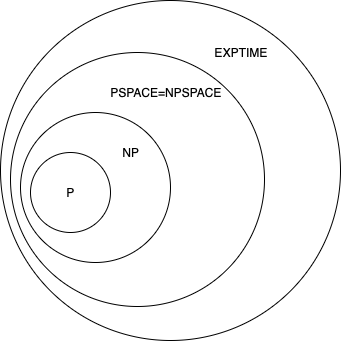
\includegraphics[scale=0.6]{NP-PSPACE}
\end{figure}
\subsubsection{PSPACE-completezza}
Un linguaggio B è PSPACE-completo se soddisfa due condizioni:
\begin{enumerate}
	\item $B \in PSPACE$
	\item $\forall \text{A in PSPACE, }A \leq_{p} B$
\end{enumerate}
Notare che è necessario effettuare la riduzione in tempo polinomiale e non in spazio polinomiale, questo perché una macchina che usa spazio polinomiale può impiegare $2^{O(n^k)}$.
\subsection{Esercizi}
1. $L \in NSPACE(n^2)$, per quale $f(n) \ L \in TIME(f(n))$

Usando il teorema Savitch, abbiamo che:
\[
	L \in NSPACE(n^2) \Rightarrow L \in SPACE(n^4) \Rightarrow TIME(2^{O(n^4)})
\]

Non usando il teorema Savitch, devo passare da NTM a TM usando la costruzione

con l'albero, quindi $L \in TIME(2^{2^{O(n^2)}})$.
\\

Bisogna controllare quale costruzione da NTM a TM restituisce il risultato migliore.
\\
2. $L \in NTIME(n^2)$, per quale $f(n) \ L \in SPACE(f(n))$

Usando il teorema di Savitch abbiamo che:


Sapendo che il tempo limita lo spazio $L \in NTIME(n^2) \Rightarrow L \in NSPACE(n^2)$, quindi:

\[
	L \in NTIME(n^2) \Rightarrow L \in NSPACE(n^2) \Rightarrow L \in SPACE(n^4)
\]

Non usando il teorema di Savitch vedo quanto spazio occupano i nastri:

\[
\left.
\begin{aligned}
&\text{nastro di input O(n)}\\
&\text{nastro di lavoro $O(n^2)$}\\
&\text{nastro guida $O(n^2)$}
\end{aligned}
\right\rbrace
\text{$\Rightarrow L \in SPACE(n^2)$}
\]

Se si parte da NTIME è consigliato usare la costruzione tramite l'albero, se si parte da 

NSPACE invece è consigliato usare il teorema di Savitch
\\
3. $A \leq_{m} \overline{A} \ A \in Turing-Riconoscibile$, cosa posso dire di $\overline{A}$

\[
	A \leq_{m} \overline{A} \Rightarrow \overline{A} \leq_{m} A \Rightarrow \overline{A} \in Turing-Riconoscibile
\]
4. $SAT \in SPACE(n) \rightarrow SAT \in TIME(2^{O(n)}$
\subsection{Algoritmo $ALL_{NFA}$}
$ALL_{NFA} = \{ <A> \ \mid A \in NFA_{\Sigma} \text{ e } L(A)=\Sigma^{\star} \}$
\\
$\overline{ALL_{NFA}} = \{ <A> \ \mid A \in NFA_{\Sigma} \text{ e } L(A) \neq \Sigma^{\star} \}$
\\\\
M: input $<A>, \ A \in NFA_{\Sigma}$

output: si se $L(A) \neq \Sigma^{\star}$

\quad \quad \quad \ \ no altrimenti
%VI PREGO RISOLVETE QUESTO SCHIFO CHE NON SONO RIUSCITO A TROVARE QUALCOSA PER FARE DI MEGLIO!!!!!!!
\begin{enumerate}
	\item $S = \varepsilon-closure$
	\item Ripeti $2^q$ volte, dove $q=|Q|$ di A (q è il massimo numero di stati della macchina deterministica di A che simula la macchina non deterministica di A)
	\begin{enumerate}[label*=\arabic*.]
		\item se S non contiene uno stato finale, accetta
		\item non deterministicamente prendi $a \in \Sigma$ e calcola $S' = \varepsilon-closure ( \bigcup_{p \in S} \delta (p,a) )$
		\item poni $S = S'$ (e ricomincia)
	\end{enumerate}
\end{enumerate}
Il più grande insieme S che considero ha q elementi, e occupa spazio O(n), dove n è la lunghezza della codifica di A: $n=|<A>| \quad n \geq q$
\\\\
$\overline{ALL_{NFA}} \in NSPACE(n)$ \newpage
\newpage
%!TEX root=../../root.tex
\section{Lezione 21}

\subsection{La classe \emph{coNP}}

\subsubsection{Definizione}
\[
	\emph{coNP} = \left\{ \ L \ | \ \overline{L} \in NP \right\}
\]
Ossia \emph{coNP} contiene tutti i linguaggi il cui complemento è in NP. \\
La classe \emph{coNP} è interessante dal punto di vista teorico poiché dimostrare che \emph{coNP} sia diversa da NP equivarrebbe a dimostrare la diversità di P ed NP. \\

\begin{align*}
	P = NP &\implies NP = \emph{coNP} \\ 
	NP \neq \emph{coNP} &\implies P \neq NP
\end{align*} 

\subsubsection{\emph{coNP}-Completezza}
\newtheorem*{def1}{Definizione}
\begin{def1}
	L è \emph{coNP}-Completo se:
	\begin{enumerate}
		\item $L \in coNP$
		\item L è \emph{coNP-Hard}, ossia $\forall A \in coNP, A \leq_{p} L$
	\end{enumerate}
\end{def1}

\subsubsection{\texorpdfstring{Il problema $\overline{TAUT}$}{Il complemento di TAUT}}
\begin{gather*}
	TAUT = \left\{ \ \varphi \ | \ \varphi \ \text{è vera per ogni assegnamento} \ \right\} \\
	\overline{TAUT} = \left\{ \ \varphi \ | \ \exists \ \text{un assegnamento che rende} \ \varphi \ \text{falsa} \ \right\}
\end{gather*}
Dimostreremo ora che $TAUT$ è \emph{coNP-Completo}.
\newtheorem*{tautcoNP}{Teorema}
\begin{tautcoNP}
	$TAUT \in coNP$
\end{tautcoNP}
\begin{proof}[Dimostrazione]
Dobbiamo mostrare che $\overline{TAUT}$, il problema della falsificabilità di formule booleane, sta in $NP$. Siamo in grado di esibirne un algoritmo (i.e. una $NTM$) che lo decide: esso è analogo a quello che decide $SAT$, soltanto che invece di controllare che vi sia un assegnamento che soddisfi la formula si controlla che ve ne sia uno che la falsifichi. 
\end{proof}

\newtheorem*{tautcoNPhard}{Teorema}
\begin{tautcoNPhard}
	$TAUT$ è coNP-completo
\end{tautcoNPhard}
\begin{proof}[Dimostrazione]
Abbiamo mostrato prima che $\overline{TAUT} \in NP \implies TAUT \in coNP$; ci resta da mostrare che $TAUT$ sia $coNP$-hard.

Sappiamo che $\forall A \in NP \quad A \leq_{p} SAT$ poiché SAT è \emph{NP-Completo}, inoltre sappiamo che se un linguaggio A si riduce ad un linguaggio B allora anche il complemento di A si può ridurre al complemento di B, quindi $\overline{A} \leq_{p} \overline{SAT}$. \\
Basta quindi dimostrare che $\overline{SAT}$ si riduce polinomialmente a TAUT per dimostrare la \emph{coNP-Hardness} di quest'ultimo. Essendo le istanze sì di $\overline{SAT}$ le formule insoddisfacibili basterà associare ad ogni formula accettata da SAT la sua negazione per avere una riduzione corretta.

\begin{align*}
	\varphi &\mapsto \neg \varphi \\
	\varphi \in \overline{SAT} &\iff \neg \varphi \in TAUT
\end{align*}

\end{proof}

\subsubsection{Relazione fra P e coNP}
Sappiamo che $P \subseteq NP$ e che $coP \subseteq coNP$, quindi dal momento che $P = coP$ possiamo affermare che:
\[
	P \subseteq NP \cap coNP
\]
Problemi in questa intersezione si rivelano spesso di interesse per la ricerca.
\subsection{Il problema FACTOR}
\subsubsection{FACTOR è in NP}
\[
	FACTOR = \{(p, u) \ | \  p,u \in \mathbb{N} \ e \ p \text{ ha un divisore} < u \} 
\]	
$FACTOR \in NP$ poichè possiamo esibire facilmente una macchina che lo verifica polinomialmente. Questa, preso $(p, u)$ e un certificato $q$, risponde sì se $q$ è un divisore di $p$ minore di $u$, no altrimenti.

\subsubsection{FACTOR è in coNP}
Per mostrare che $FACTOR \in coNP$ dimostriamo, esibendo un verificatore, che $\overline{FACTOR} \in NP$.

\[
	\overline{FACTOR} = \{(p, u) \ | \  p,u \in \mathbb{N} \ e \ p \text{ non ha un divisore} < u \} 
\]	
$\overline{FACTOR} \in NP$ poichè possiamo esibire facilmente una macchina che lo verifica polinomialmente. Il verificatore prende in input $(p, u)$ e un certificato composto da una lista $p_1,p_2,...,p_k$, con ciascun $p_i < u < p$. Esso risponde sì se tali numeri primi rappresentano una scomposizione in fattori primi di $p = p_1 p_2 ... p_k$, no altrimenti.

Nel peggiore dei casi, i numeri primi in $p_1, p_2, ..., p_k$ sono tutti $2$, il più piccolo numero primo, e $k$ è tale che $2^k < u$. Quindi $k = O(log \ u)$, con $u$ non maggiore di $p$. Di conseguenza la lunghezza del certificato nel peggiore dei casi è uguale a $k log \ 2 = k \cdot 1 = O(log \ u) = O(log \ p)$, ossia polinomiale nella lunghezza della codifica di $p$. 

Il verificatore deve semplicemente controllare che il prodotto dei primi sia uguale a $p$, una operazione banalmente polinomiale. Quindi il verificatore è effettivamente polinomiale.

\subsubsection{Prova di NP = coNP (non verificata)}
\[
	\text{FACTOR è NP-completo} \implies NP = coNP
\]
Purtroppo l'ipotesi $\text{FACTOR è NP-completo}$ non è verificata, ed è considerata altamente improbabile. Ci avrebbe permesso di dimostrare $NP = coNP$ per doppia inclusione come segue:
\\
\newtheorem*{NPcoNP}{Prima inclusione}
\begin{NPcoNP}
$$NP \subseteq coNP$$
\end{NPcoNP}

\begin{proof}[Dimostrazione]

\begin{align*}
	L \in NP \implies L \leq_{p} FACTOR \implies \overline{L} \leq_{p} \overline{FACTOR} \\
	\overline{FACTOR} \in NP \implies \overline{L} \in NP \implies L \in coNP
\end{align*}

\end{proof}

\newtheorem*{coNPNP}{Seconda inclusione}
\begin{coNPNP}
$$coNP \subseteq NP$$
\end{coNPNP}
\begin{proof}[Dimostrazione]

\begin{gather*}
	L \in coNP \implies \overline{L} \in NP \\ 
	\overline{L} \leq_{p} FACTOR \iff L \leq_{p} \overline{FACTOR} \\
	\overline{FACTOR} \in NP \land L \leq_p \overline{FACTOR} \implies L \in NP
\end{gather*}

\end{proof}

\subsection{Il problema del Grafo Isomorfo}

\theoremstyle{definition}
\newtheorem*{def2}{Definizione}
\begin{def2}[Grafi isomorfi]
	Dati due grafi $G, G'$ diciamo che essi sono \emph{isomorfi} se esiste una funzione $f: V_G \to V_{G'}$ biettiva tale che	
	$$ \{ u, v \} \in E_G \iff \{ f(u), f(v) \} \in E_{G'}$$
	ovvero tale che, se due nodi in $G'$ sono connessi, allora lo sono anche i nodi associati da $f$ in $G'$.
\end{def2}

Sulla base di questa definizione, ci chiediamo se stabilire l'isomorfismo tra grafi sia un problema contenuto in $NP$. Introduciamo quindi il linguaggio $GI$:

\[
	GI = \{ \langle G, G' \rangle \ \mid \ G \text{ è isomorfo a } G'\}
\]

\theoremstyle{plain}
\newtheorem*{theo1}{Teorema}
\begin{theo1} 
$GI \in NP$
\end{theo1}

\begin{proof}[Dimostrazione]
	Mostriamo un verificatore polinomiale per $GI$:
	\\

	$V_{GI}$:
	\begin{description}
		\item[input] $\langle G, G' \rangle$ e il certificato $c = (u_1, f(u_1)), ..., (u_k, f(u_k))$, che è la codifica \\
		"per esteso" di $f$

		\item[output] sì se $\langle G, G' \rangle \in GI$, no altrimenti

		\item[descrizione] Controlla che per ogni arco $\{ u_i, u_j \} \in E_G$ l'arco $\{ f(u_i), f(u_j) \}$ stia in $E_{G'}$.
	\end{description}
\end{proof}

Sappiamo quindi che $GI \in NP$, ma purtroppo non possiamo dire se anche $GI \in P$ nè tantomeno se $GI$ sia un problema $NP$-completo.

\subsection{Esercizi}

\newtheorem*{exc1}{Esercizio 1}
\begin{exc1}
	Se $C \in TIME(n^3)$ e $D \leq_p C$ allora sappiamo che $D \in TIME(f(n))$ per qualche $f(n)$. Cosa possiamo dire su $f(n)$?
\end{exc1}

Se $D \leq_p C$ allora esiste una qualche funzione di riduzione, che indichiamo con $g$, che è calcolabile polinomialmente. Sia $T_g \in TM$ la macchina che la calcola, allora per quanto detto vale $t_{T_g}(n) = O(n^k)$. Sia inoltre $T_c \in TM$ la macchina che decide $C$ e $T_d \in TM$ la macchina che decide $D$. Essa sarà costruita nel seguente modo:

\begin{figure}[H]
	\centering
	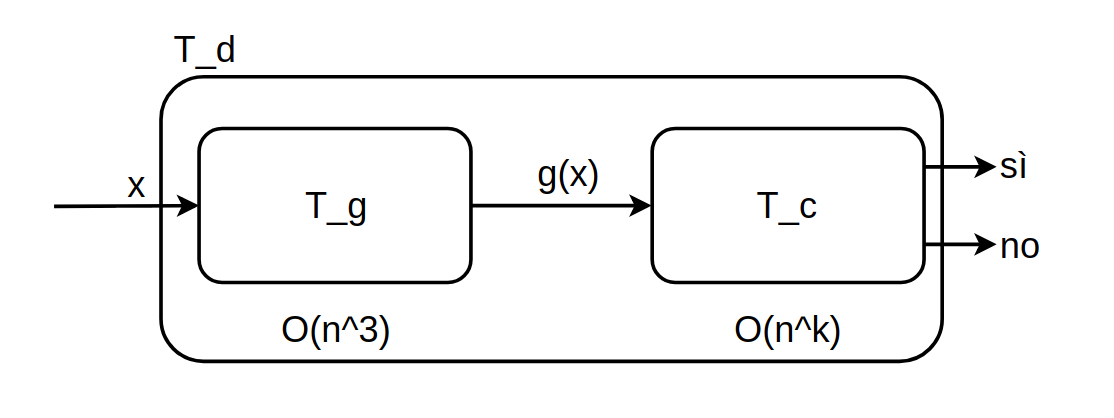
\includegraphics[width=\textwidth]{riduzione-esercizio}
\end{figure}

Sia $n = |x|$ la dimensione dell'input; poiché il tempo limita lo spazio, possiamo dire che $|g(x)| = O(n^k)$. Da ciò discende che $T_c$ riceverà input di dimensione $O(n^k)$, e quindi $t_{T_d}(n) = t_{T_g}(n) + t_{T_c}(n^k) = O(n^k) + O((n^k)^3) = O(n^k) + O(n^{3k}) = O(n^{3k})$. Concludiamo quindi che $D \in TIME(n^{3k})$.

\newtheorem*{exc2}{Esercizio 2}
\begin{exc2}
Correggere le seguenti affermazioni:
\end{exc2}
\begin{enumerate}
			\item per dimostrare che $X \in NP$-completo si deve dimostrare:
				\begin{description}
					\item \textit{1.} $X \in NP$,
					\item \textit{2.} $X \leq_p Y$ per un $Y \in NP$-completo.
				\end{description}
				In questa affermazione è sbagliato dire $X \leq_p Y$ per un $Y \in NP$-completo. $X$ è $NP$-completo se un problema $NP$-completo può essere ridotto ad esso, quindi va corretta con $Y \leq_p X$ per un $Y \in NP$-completo.
			
			\item Esiste un problema $NP$-completo che si risolve in tempo polinomiale deterministico ma questo non è vero per $SAT$.\\
			Se esistesse un problema $NP$-completo polinomiale allora tutti i problemi $NP$-completi si ridurrebbero a questo problema. Ma anche $SAT \in NP$-completo e quindi anche esso sarebbe riducibile a questo problema.
						
			\item $X \leq_p SAT \ \forall X \in NP$-hard\\
			L'affermazione non è vera in generale, poiché NP-hard è una classe più estesa di NP, e poiché SAT è NP-completo, l'affermazione è vera per gli $X \in NP$.
		\end{enumerate}


\newtheorem*{exc3}{Esercizio 3}
\begin{exc3}
Siano $INDSET, VC$ i seguenti linguaggi:
\begin{gather*}
	INDSET = \{\langle G,k \rangle  \ \mid  \ G \ \text{ha un indipendent set di k vertici}\} \\
	VC = \{\langle G, k \rangle  \ \mid  \ \text{esiste un vertex cover di k vertici per } G\}
\end{gather*}
Esibire una riduzione $INDSET \leq_p VC$, sapendo che $VC$ è $NP$-completo
\end{exc3}
Vogliamo esibire una riduzione $\langle G,k \rangle  \xmapsto{f} \langle G', k' \rangle $ tale che 
\[
	G \text{ ha un indipendent set di k vertici} \iff G' \text{ ha un vertex cover di k' vertici}
\]
La $f$ di riduzione costruisce una istanza $\langle G', k' \rangle$ con $G'=G$ e $k'=|V|-k$. Mostriamo che questa è una riduzione corretta:
\begin{gather*}
	A \subseteq V_G \text{ è un indipendent set di} \  k \ \text{vertici } \\
	\iff \\
	V_G-A \text{ è un vertex cover di } |V|-k \text{ vertici}
\end{gather*}
$\implies: \{u,w\} \in E$ allora certamente $u$ e $w$ non possono essere entrambi in $A$, quindi $u \in V-A$ oppure $w \in V-A$, allora per ogni arco uno degli estremi sta in $V-A$, che quindi è un vertex cover. Poiché $|A| = k$, $|V-A| = |V|-k$, quindi abbiamo dimostrato che $V-A$ è un vertex cover di $|V| - k$ vertici.
\\
$\impliedby: $ Supponiamo per assurdo che $V_G - A$ sia un vertex cover, e che $A$ non sia un independent set. Se $A$ non fosse un independent set, allora $\exists u, w \in A$ tali che $\{u, w\} \in E$. Ma allora l'arco $\{u, w\}$ sarebbe "scoperto", in quanto nè $u$ nè $w$ stanno nel vertex cover, quindi $V_G - A$ non sarebbe un vertex cover (assurdo).

\end{document}